\documentclass[12pt]{article}

%------------------------------------------%
%                Packages
%------------------------------------------%
%These are the packages that we will use in our latex document. 
\usepackage{clipboard}%For copy past text in different parts of document
\usepackage{amsmath, amssymb,mathrsfs} %For using math
\usepackage{color}
\usepackage{enumitem}
\usepackage{graphicx}
\usepackage{grffile}
\usepackage[utf8]{inputenx}% For proper input encoding
\usepackage{mathptmx}
\usepackage{pdflscape}
\usepackage{soul}
%\usepackage{libertine}% Linux Libertine, may favourite text font
%\usepackage{mathpazo}
\usepackage[euler-digits]{eulervm}% A pretty math font

%\usepackage{fontspec}
%\usepackage{unicode-math}

%\setmainfont{Linux Libertine O}

%\newcommand{\setlibertinemath}{%
% use Libertine for the letters
%\setmathfont[range=\mathit/{latin,Latin,num,Greek,greek}]{Linux Libertine O Italic}
%\setmathfont[range=\mathup/{latin,Latin,num,Greek,greek}]{Linux Libertine O}
%\setmathfont[range=\mathbfup/{latin,Latin,num,Greek,greek}]{Linux Libertine O Bold}
%\setmathfont[range={"2202}]{Linux Libertine O}% "02202 = \partial % doesn't work
%\setmathfont[range={"221E}]{Linux Libertine O}% "0221E = \infty
% etc. (list should be completed depending on needs)
%}



%%% ABSTRACT
\usepackage{abstract}
\renewcommand{\abstractname}{}    % clear the title
\renewcommand{\absnamepos}{empty} % originally center

%%% PAGE DIMENSIONS
\usepackage[margin=1in]{geometry} %For controlling the dimensions. Very useful for Posters, etc
% PAPER SIZE
\setlength\paperheight{11in}
\setlength\paperwidth{8.5in}
% MARGINS 
%\topmargin=-0.5in
\parskip=0pt
%\setlength\textwidth{135.5mm}
%\setlength\textheight{200mm}
%\setlength\topmargin{-10pt}
%\setlength\oddsidemargin{14mm}
%\setlength\evensidemargin{\oddsidemargin}
%\setlength\headheight{24pt}
%\setlength\headsep{14pt}
%\setlength\topskip{11.74pt}
%\setlength\maxdepth{.5\topskip}
%\setlength\footskip{15pt}

%%% HEADERS AND FOOTERS
\usepackage{fancyhdr}
%\pagestyle{plain} % options: empty , plain , fancy
%\renewcommand{\headrulewidth}{0pt} % customise the layout...
%\lhead{}\chead{}\rhead{}
%\lfoot{}\cfoot{\thepage}\rfoot{}

%%% SECTION TITLE APPEARANCE
%\usepackage{sectsty}
%%\sectionfont{\large}
%\sectionfont{\normalsize}
%\subsectionfont{\small}
%\paragraphfont{\small}
%\allsectionsfont{\mdseries\upshape 
%        \sectionrule{15pt}{0pt}{-5pt}{1pt} }
\usepackage{titlesec}
\titleformat*{\section}{\normalsize\bfseries}
\titleformat*{\subsection}{\small\bfseries}
\titleformat*{\subsubsection}{\small\bfseries}
\titleformat*{\paragraph}{\small\bfseries}
\titleformat*{\subparagraph}{\small\bfseries}
\titlespacing\section{0pt}{6pt plus 4pt minus 2pt}{0pt plus 2pt minus 2pt}
\titlespacing\subsection{0pt}{6pt plus 4pt minus 2pt}{0pt plus 2pt minus 2pt}
\titlespacing\subsubsection{0pt}{6pt plus 4pt minus 2pt}{0pt plus 2pt minus 2pt}
\titlespacing\paragraph{0pt}{6pt plus 4pt minus 2pt}{6pt plus 2pt minus 2pt}

%%% CITATIONS
\usepackage[authoryear]{natbib}	%Bibliography package. It handles citations and can easily change formats. This is done at the end of the document
\usepackage{multibib}
\newcites{App}{Appendix References}%  \citelatex, \nocitelatex, ...
\newcites{Ref}{References in Referee Replies}%  \citelatex, \nocitelatex, ...
\newcites{Main}{References}%  \citelatex, \nocitelatex, ...

\setcitestyle{aysep={}} 
%------------------------------------------%
%     Tables 
%------------------------------------------%
\usepackage{accents}
\usepackage{adjustbox} %Handles resizing of tables, figures, etc. Based off of page and/or line width/height 
\usepackage{bbm}
\usepackage{bm}
\usepackage{booktabs}% For Pretty tables
\usepackage{caption} %\captionsetup[figure]{justification=raggedright,singlelinecheck=off}
\captionsetup[table]{labelsep=period}
\captionsetup{labelsep=period}
\usepackage{chngpage} 
\usepackage{comment}
\usepackage{dcolumn}
%\usepackage{everypage}%For page numbers on rotated pages%Functionality added to latex
%\usepackage{float}
\usepackage[capposition=top]{floatrow}
\usepackage{morefloats}
\usepackage{multicol}
\usepackage{multirow}
\usepackage{placeins}% To Create Float Barriers so the tables will stay in their sections
\usepackage[list=true]{subcaption} %For having multiple figures within the same one. Figure 1, with part (a) and (b) %\setcounter{lofdepth}{2}
\usepackage{threeparttable}% For Notes below table
\usepackage{rotating}% To Rotate Table
\usepackage{setspace} %Single, Double Space, etc 
\usepackage{siunitx} %This aligns tables by their decimal and handles processing of the numbers within the tables
  \sisetup{
    detect-mode,
    group-digits      = false,
    input-symbols     = {( ) [ ] - +},
    table-align-text-post = false,
    input-signs             = ,
    %parse-numbers=false,
    %scientific-notation = true,
        %round-mode              = places,
        %round-precision         = 2,
    %input-ignore={,},
    input-decimal-markers={.},
    group-separator={,},
    %group-minimum-digits={4},
    %group-four-digits = true,
	separate-uncertainty=true,
	%zero-decimal-to-integer=true,
   } 
%------------------------------------------%
%     Formatting options 
%------------------------------------------%

\AtBeginDocument{
    \addtolength{\abovedisplayskip}{-1.0ex}
    \addtolength{\abovedisplayshortskip}{-1.0ex}
    \addtolength{\belowdisplayskip}{-1.0ex}
    \addtolength{\belowdisplayshortskip}{-1.0ex}
}
\setlength{\parskip}{\smallskipamount}%med
%\setlength{\parindent}{0pt}
\DeclareCaptionLabelFormat{blank}{}
\DeclareCaptionFormat{myformat}{
    \begin{varwidth}{\linewidth}
        \centering
        #1#2#3%
    \end{varwidth}
}
\usepackage{silence}
\WarningFilter*{latex}{Text page \thepage\space contains only floats}
\WarningFilter*{caption}{Ambiguous sub-caption}
\WarningFilter*{natbib}{Citation}
\WarningFilter{natbib}{Citation}

%------------------------------------------%
%     Hyper Ref 
%------------------------------------------%
%\usepackage{silence}
%\WarningFilter{hyperref}{You have enabled option `breaklinks'.}
\usepackage[unicode=true,pdfusetitle,bookmarks=true,bookmarksnumbered=false,bookmarksopen=false,breaklinks=true,pdfborder={0 0 1},backref=false,colorlinks=true,citecolor=black,allcolors=black,hyperfootnotes=true]{hyperref}
%\usepackage[unicode=true,pdfusetitle,bookmarks=true,bookmarksnumbered=false,bookmarksopen=false,breaklinks=true,pdfborder={0 0 1},backref=false,colorlinks=true,citecolor=black,hyperfootnotes=true]{hyperref}
\def\UrlBreaks{\do\/\do-\do.\do=\do_\do?\do\&\do\%\do\a\do\b\do\c\do\d\do\e\do\f\do\g\do\h\do\i\do\j\do\k\do\l\do\m\do\n\do\o\do\p\do\q\do\r\do\s\do\t\do\u\do\v\do\w\do\x\do\y\do\z\do\A\do\B\do\C\do\D\do\E\do\F\do\G\do\H\do\I\do\J\do\K\do\L\do\M\do\N\do\O\do\P\do\Q\do\R\do\S\do\T\do\U\do\V\do\W\do\X\do\Y\do\Z\do\0\do\1\do\2\do\3\do\4\do\5\do\6\do\7\do\8\do\9} 
%\usepackage[hyphenbreaks]{breakurl}
% hyperef does not work with beamer (as far as I know) so comment this out if you are using it. 
% Also leave the hyperfootnotes as false as when they are true they oddly clash with the caption or subcaption package.


%------------------------------------------%
%    Appendix
%------------------------------------------%
%\usepackage[titletoc]{appendix}
\usepackage[toc,page,header]{appendix}
\usepackage{minitoc}

%------------------------------------------%
%    To Do Notes
%------------------------------------------%

%\usepackage[colorinlistoftodos,prependcaption,textsize=tiny]{todonotes}
\usepackage{xcolor}
\usepackage{xargs}
%Use \todo to create a general todo item for anyone
%Something for Chris to do
%\newcommandx{\todochris}[2][1=]{\todo[linecolor=green,backgroundcolor=green!25,bordercolor=yellow,#1]{Chris: #2}}
%\newcommandx{\todokk}[2][1=]{\todo[linecolor=green,backgroundcolor=green!25,bordercolor=yellow,#1]{Chris: #2}}
%Something for Anthony to do
%\newcommandx{\todoanthony}[2][1=]{\todo[linecolor=green,backgroundcolor=green!25,bordercolor=yellow,#1]{Anthony: #2}}
% To just make a comment use this
%\newcommandx{\todocomment}[2][1=]{\todo[linecolor=yellow,backgroundcolor=yellow!25,bordercolor=cyan,#1]{Comment: #2}}
\renewcommand{\thefootnote}{\fnsymbol{footnote}}

\setlength{\marginparwidth}{2cm}
\usepackage[colorinlistoftodos]{todonotes}
\usepackage{epigraph}
\setlength \epigraphwidth {\linewidth}
\setlength \epigraphrule {0pt}
\AtBeginDocument{\renewcommand {\epigraphflush}{center}}
\renewcommand {\sourceflush} {center}

%------------------------------------------%
%              Custom Commands 
%------------------------------------------%
%These are the custom commands that I use in the latex document

\newcommand\iid{i.i.d.} %Makes iid a command
\newcommand\pN{\mathcal{N}} %Makes the natural numbers a command

\setcounter{MaxMatrixCols}{20}

\newtheorem{theorem}{Theorem}%[section]
\newtheorem{lemma}[theorem]{Lemma}
\newtheorem{proposition}[theorem]{Proposition}
\newtheorem{corollary}[theorem]{Corollary}
\newtheorem{assumption}[theorem]{Assumption}
\newenvironment{proof}{\paragraph{Proof:}}{\hfill$\square$ \\} %This fixes the problem with dynamic tables for some reason

%For Page Numbers while rotated
%\newlength{\hfoot}
%\newlength{\vfoot}
%\AddEverypageHook{\ifdim\textwidth=\linewidth\relax
%\else\setlength{\hfoot}{-\topmargin}%
%\addtolength{\hfoot}{-\headheight}%
%\addtolength{\hfoot}{-\headsep}%
%\addtolength{\hfoot}{-.5\linewidth}%
%\ifodd\value{page}\setlength{\vfoot}{\oddsidemargin}%
%\else\setlength{\vfoot}{\evensidemargin}\fi%
%\addtolength{\vfoot}{\textheight}%
%\addtolength{\vfoot}{\footskip}%
%\raisebox{\hfoot}[0pt][0pt]{\rlap{\hspace{\vfoot}\rotatebox[origin=cB]{90}{\thepage}}}\fi}
%http://tex.stackexchange.com/questions/209685/landscape-mode-and-page-numbering

%For figure notes
\newcommand{\Ftext}[1]{%
    \begin{minipage}[b]{1.0\linewidth}
        \vspace{2mm}
        \begin{flushleft}
            \subcaption*{#1}
        \end{flushleft}
    \end{minipage}
 }
\newcommand{\Fnote}[1]{\Ftext{\text{Notes:~}~#1}}
\newcommand{\FnoteScript}[1]{\Ftext{\text{\scriptsize{Notes:}~}~#1}}
\newcommand{\FnoteFoot}[1]{\Ftext{\text{\footnotesize{Notes:}~}~#1}}

%Math
\newcommand{\ev}[1]{\mathop{\mathbb E\,} \left[#1\right]}
\newcommand{\indep}{\perp \!\!\! \perp}
\newcommand{\var}{\operatorname{var}}
\newcommand{\cov}{\operatorname{cov}}

%------------------------------------------%
%      Matter Related to Table Creation 
%------------------------------------------%
%This helps with custom automatic tables. It uses latex  functions
%http://www.jwe.cc/2012/03/stata-latex-tables-estout/
%http://repec.org/bocode/e/estout/estout.html

% *****************************************************************
% Estout related things
% *****************************************************************

% Added due to changes in TexLive 2022 breaking code
%https://www.overleaf.com/blog/tex-live-2022-now-available
%https://tex.stackexchange.com/questions/567985/problems-with-inputtable-tex-hline-after-2020-fall-latex-release
\makeatletter
%%primitive input in tabular
\AddToHook{env/tabular/begin}{\let\estinput=\@@input}
\makeatother
%\let\estinput=\@@input % define a new input command so that we can still flatten the document

\newcommand{\estwide}[3]{
    \vspace{.25ex}{
      \textsymbols% Note the added command here
      \begin{tabular*}
      {\textwidth}{@{\hskip\tabcolsep\extracolsep\fill}l*{#2}{#3}}
      \toprule
      \estinput #1 
      \bottomrule
      \addlinespace[.75ex]
      \end{tabular*}
      }
    } 

\newcommand{\estauto}[3]{
    \vspace{.25ex}{
      \textsymbols% Note the added command here
      \begin{tabular}{l*{#2}{#3}}
      \toprule
      \estinput #1 
      \bottomrule
      \addlinespace[.75ex]
      \end{tabular}
      }
    }

% Allow line breaks with \\ in specialcells
\newcommand{\specialcell}[2][c]{%
    \begin{tabular}[#1]{@{}c@{}}#2\end{tabular}
}
\DeclareUnicodeCharacter{00A0}{ }
% *****************************************************************
% Custom subcaptions
% *****************************************************************
% Note/Source/Text after Tables
% The new approach using threeparttables to generate notes that are the exact width of the table.
\newcommand{\Figtext}[1]{%
  \begin{tablenotes}[para,flushleft]
  %\hspace{6pt}
  %\hangindent=1.75em
  #1
  \end{tablenotes}
  }
\newcommand{\Fignote}[1]{\Figtext{\text{Notes:~}~#1}}
\newcommand{\Figsource}[1]{\Figtext{\text{Source:~}~#1}}
\newcommand{\Starnote}{\Figtext{Point estimates marked ***, **, and * are statistically significant at the 1, 5, and 10 percent levels, respectively.}}% Add significance note with \starnote
% If you are using hyper-ref (recommended), this command must go after all 
% other package inclusions (from the hyperref package documentation).
% The purpose of hyperref is to make the PDF created extensively
% cross-referenced.

\usepackage{ifthen}
\newboolean{stars_on}
\setboolean{stars_on}{false} % or {false}
\ifthenelse{\boolean{stars_on}}
{%
  % Text to include when stars_on is true
  \newcommand{\sym}[1]{\rlap{#1}}
  \newcommand{\nlsym}[1]{\rlap{\append{}{*}{#1}}}
  \newcommand{\pvaluenote}{* p $<$ 0.1, ** p $<$ 0.05, *** p $<$ 0.01. }
}
{%
  % Text to include when stars_on is false
  \newcommand{\sym}[1]{\rlap{~}}
  \newcommand{\nlsym}[1]{\rlap{\append{}{~}{#1}}}
  \newcommand{\pvaluenote}{}

}
 %Allows for fancy stars in tables that also works in beamer
% %Allows for fancy stars in tables that also works in beamer

% Create a function that works for the non-linear symbols
%\newcommand{\nlsym}[1]{\rlap{\append{}{*}{#1}}} %Allows for fancy stars in tables that also works in beamer
 %Allows for fancy stars in tables that also works in beamer

% Character substitution that prints brackets and the minus symbol in text mode. Thanks to David Carlisle
\def\yyy{%
  \bgroup\uccode`\~\expandafter`\string-%
  \uppercase{\egroup\edef~{\noexpand\text{\llap{\textendash}\relax}}}%
  \mathcode\expandafter`\string-"8000 }

\def\xxxl#1{%
\bgroup\uccode`\~\expandafter`\string#1%
\uppercase{\egroup\edef~{\noexpand\text{\noexpand\llap{\string#1}}}}%
\mathcode\expandafter`\string#1"8000 }

\def\xxxr#1{%
\bgroup\uccode`\~\expandafter`\string#1%
\uppercase{\egroup\edef~{\noexpand\text{\noexpand\rlap{\string#1}}}}%
\mathcode\expandafter`\string#1"8000 }

\def\textsymbols{\xxxl[\xxxr]\xxxl(\xxxr)\yyy}


%Protects against odd minus sign errors within the tables
\catcode`_11
\protected\def \c__siunitx_minus_tl {$-$}
\catcode`_ 8 

%-----------Tables-------------%
% This Section is needed to make the tables work with amsmath. But because of the \( being open and having no match, Sublime Text thinks that everything after it (all text) is in math mode and hence changes the text color. This annoys me so the only ``solution'' is to just place this preamble here. It seems to work still. 
\makeatletter 
\edef\originalbmathcode{%
    \noexpand\mathchardef\noexpand\@tempa\the\mathcode`\(\relax} %\)

\def\resetMathstrut@{%
  \setbox\z@\hbox{%
    \originalbmathcode

    \def\@tempb##1"##2##3{\the\textfont"##3\char"}%
    \expandafter\@tempb\meaning\@tempa \relax
  }%
  \ht\Mathstrutbox@\ht\z@ \dp\Mathstrutbox@\dp\z@
}
\makeatother %./tables.tex:25: LaTeX Error: Bad math environment delimiter. [\)]
\usepackage{xparse}

\ExplSyntaxOn
\DeclareExpandableDocumentCommand{\append}{mmm}
 {
  #1\prg_replicate:nn{#3}{#2}
 }
\ExplSyntaxOff

\doublespacing

%------------------------------------------%
%   Referee Replies
%------------------------------------------%
\usepackage{csquotes}
\usepackage{ragged2e}
\usepackage{microtype,xparse,tcolorbox}

% Make the "Part I" text invisible
\renewcommand \thepart{}
\renewcommand \partname{}

\begin{document}

%------------------------------------------%
%     Title Page
%------------------------------------------%

\begin{titlepage}
    \vspace*{.25cm}
    \begin{center}
        \renewcommand{\thefootnote}{\fnsymbol{footnote}}
        \textbf{
        \noindent\LARGE
        \title
         ~Later-life Mortality and \\ the Repeal of Federal Prohibition \footnote{We appreciate feedback from the editor, three anonymous referees, Shari Eli, Kevin Schnepel, and Simon Woodcock. 
         We also gratefully acknowledge research support from the National University of Singapore and the Social Sciences and Humanities Research Council of Canada. 
         Jacks: National University of Singapore and CEPR (dsjacks@gmail.com); Pendakur: Simon Fraser University (pendakur@sfu.ca); Shigeoka: University of Tokyo and IZA (\href{mailto:hitoshi.shigeoka@gmail.com}{hitoshi.shigeoka@gmail.com}); Wray: University of Southern Denmark and IZA (wray@sam.sdu.dk).}
        }
        
        \vspace{.7cm}
        {\large 
        \hspace{-0.75cm} David S. Jacks \hspace{4.5cm} Krishna Pendakur \\ 
        \vspace{-0.25cm} 
        \hspace{-0.75cm} National University of  \hspace{3cm} Simon Fraser University \\ 
        \vspace{-0.5cm}
        \hspace{-8.5cm} Singapore and CEPR \\
        \vspace{0.5cm}
        \hspace{-1.25cm} Hitoshi Shigeoka \hspace{4.25cm} Anthony Wray \\ 
        \vspace{-0.25cm}
        \hspace{-0.5cm}
        University of Tokyo and IZA \hspace{1.5cm} University of Southern Denmark \\
        \vspace{-0.25cm} 
        \hspace{7cm} and IZA} \\
        \vspace{.5cm}
        {\large May 9, 2024}\\ %\today
    \end{center}
    
    \begin{abstract}
    \begin{normalsize}
    \begin{singlespace}

    \noindent
	Despite a recent and dramatic re-evaluation of the health consequences of alcohol consumption, very little is known about the effects of in utero exposure to alcohol on long-run outcomes such as later-life mortality. 
    Here, we investigate how state by year variation in alcohol control arising from the repeal of federal prohibition affects mortality for cohorts born in the 1930s. 
    We find that individuals born in wet states experienced higher later-life mortality than individuals born in dry states, translating into a 3.3\% increase in mortality rates between 1990 and 2004 for affected cohorts.
	\end{singlespace}
    \end{normalsize}
    \end{abstract}
    
    \noindent\textbf{JEL:} H73, I18, J18, N32
    \vspace{.6cm} 
    
    \noindent\textbf{Keywords:} Alcohol, federal prohibition, in utero exposure, later-life mortality
    \setcounter{footnote}{0}
    

\end{titlepage}
\newpage

\doparttoc % Tell to minitoc to generate a toc for the parts
\faketableofcontents % Run a fake tableofcontents command for the partocs

%------------------------------------------%
%                Main text
%------------------------------------------%
\FloatBarrier
\renewcommand{\thefootnote}{\arabic{footnote}}

\setlength{\floatsep}{10pt}
\setlength{\textfloatsep}{0pt}

%------------------------------------------%
%      Introduction
%------------------------------------------%

\onehalfspacing 
\section{Introduction} \label{sec:intro}

While the harms of excessive alcohol consumption have long been understood \citepMain{rehm_risks_2011}, only very recently has there been a dramatic re-evaluation of the health impacts of moderate levels of consumption. 
One of the starkest examples of this re-assessment comes from a Global Burden of Death, Injuries, and Risk Factors (GBD) study which concludes that the ``level of [alcohol] consumption that minimizes health loss is zero'' \citepMain{gbd_2016_alcohol_collaborators_alcohol_2018}.  
Likewise, the personal and social harms of alcohol use have been ranked the highest among all drugs, including heroin and methamphetamine \citepMain{nutt_drink_2020}. 
And this is not a story merely about the accumulation of academic and scientific evidence as consumers have responded in kind: worldwide, the share of active drinkers has been in decline since 2000 while per-capita use is declining in former strongholds of drinking activity and culture like the Anglosphere and Europe \citepMain{poznyak_global_2018}. 

The detrimental effects of in utero alcohol exposure on childhood development -- first proposed by \citeMain{lemoine_les_1968} and definitively established by \citeMain{clarren_fetal_1978} -- has been amply demonstrated and is now widely appreciated. 
However, to our knowledge, there is very little evidence on the later-life mortality effects of in utero exposure to alcohol. 
And while there is a well-established literature in economics considering quasi-experiments that substantially eased or restricted access to alcohol, these policy changes are oftentimes short-lived, limited in their geographic scope, or too recent in the past to speak to the effects of alcohol exposure on later-life mortality \citepMain{carpenter_effect_2009,carpenter_minimum_2011,aizer_intergenerational_2014,nilsson_alcohol_2017,almond_childhood_2018,kueng_long-run_2021}. 

This paper addresses these issues head on and fills the gap in our understanding by assessing the long-run effects of federal prohibition's repeal in the 1930s on later-life mortality and offering up potential physiological mechanisms for the same. 
In so doing, we confront a common misunderstanding about the nature of federal prohibition: there was no uniform policy change with restrictions on alcohol ``turning off'' precisely in December 1933 when federal prohibition was repealed. 
Instead, the decentralized nature of American government and the political concessions necessary to bring about repeal worked to ensure that there was ample geographic and temporal heterogeneity in restrictions on alcohol well after federal prohibition ended.

Our goal is to identify the causal intent-to-treat effects of in utero exposure to alcohol on later-life mortality. 
To do so, we use data on state by year variation in alcohol prohibition coupled with annual death rates from 1990 to 2004 for cohorts born in the 1930s. 
We conduct event-study analysis in the context of a difference-in-differences research design that exploits the staggered timing of federal prohibition's repeal. 
We find evidence that allowing for legal alcohol sales (that is, transitioning from ``dry'' to ``wet'' status) at the state level is associated with a 3.3\% increase in mortality rates between 1990 and 2004. 
Critically, we show that these effects are localized to the in utero period as cohorts which were already in early childhood when states became wet do not see equivalent increases in later-life mortality.
Our results would thus seem to rule out other potential non-physiological mechanisms such as domestic violence or parental investment which should not be discontinuous in their effects at the time of a cohort's birth.\footnote{Earlier work which examines federal repeal's effect on infant mortality \citepMain{jacks_infant_2021} also found no systematic link between easing restrictions on the availability of alcohol and subsequent fertility, either in the aggregate US population or across SES. The latter result in particular suggests a limited role for selection into pregnancy in driving the results here.}

Instead, we speak to the potential physiological mechanisms underlying this result by examining repeal's effect on cause-specific mortality rates. 
We find that in utero exposure to alcohol availability is associated with increases in mortality rates for heart disease and stroke in later life. 
We also have good reasons to believe that these results are not spurious: we find no corresponding increase in later-life mortality arising from motor vehicle accidents, a cause of death which is plausibly unrelated to in utero alcohol exposure. 
We furthermore demonstrate that our results are unaffected when we control for exposure to both the Great Depression and New Deal spending. 
This suggests that our results are not driven by other confounding events which may be correlated with the timing of prohibition's repeal across states and years. 
Finally, we examine potential heterogeneity along the lines of sex and race, finding that females and males as well as non-white and white people are similarly affected, suggesting our baseline results are not driven by other mechanisms such as differential healthcare access. 

This paper contributes to the literature in two ways. 
First, we present causal evidence that the well-known, detrimental effects of in utero exposure to alcohol also extend to mortality in later life. 
Prior work has documented in utero effects of potential alcohol exposure on contemporaneous infant mortality \citepMain{jacks_infant_2021} and subsequent labor market outcomes \citepMain{nilsson_alcohol_2017}, but not on outcomes observed in later life.
Relatedly, localized prohibitions of alcohol in the US prior to federal prohibition in 1920 had effects on contemporaneous alcohol-related mortality \citepMain{law_did_2020}, education and obesity \citepMain{evans_developmental_2016}, and longevity \citepMain{noghanibehambari_utero_2023}.\footnote{We discuss how the \citeMain{noghanibehambari_utero_2023} longevity result relate to our findings in Section~\ref{sec:results-aggregate}.}
While we would expect efforts to reduce alcohol consumption to have opposite signed effects to the repeal of prohibition, it is an open question whether the absolute magnitudes of the two policies’ effects on mortality are in fact the same. 
Thus, it is important to evaluate both sets of policies. 
Furthermore, to the extent that the weakest of embryos were culled due to repeal increasing infant mortality as in \citeMain{jacks_infant_2021} or other forms of post-natal mortality, the scarring effect estimated in this paper may actually prove to be a lower bound.

Second, we add to a burgeoning literature on the consequences for later-life mortality of the multiple economic shocks and policy interventions occurring in the US during the 1930s. 
\citeMain{aizer_long-run_2016} find that the Mothers' Pension program increased longevity for male children of recipients. 
\citeMain{duque_early-life_2023} find that children most exposed to the deprivations of the Great Depression experienced higher mortality in later life, a result which is likely driven by the Great Depression's effect on accelerated epigenetic aging \citepMain{schmitz_utero_2022}. 
At the same time, \citeMain{jou_relief_2024} find that after accounting for the endogeneity of New Deal spending, the latter moderated -- and in some instances fully reversed -- the negative effects of the Great Depression. 

Understanding the effects of repeal might also be important with respect to contemporary policy issues related to alcohol. 
The US Surgeon General's initial warning about the risks associated with alcohol consumption during pregnancy was issued in 1981. 
But in the 1930s, the general public had little definitive knowledge of the potential negative effects of alcohol consumption during pregnancy on child development \citepMain{warner_effects_1975}.\footnote{\citeMain{pauly_is_1994} discusses efforts to promote the normalization of alcohol consumption during repeal.}
Thus, our estimates are potentially not driven by differences in avoidance behaviours by mothers of different socioeconomic status. 
Finally, we note that the scope for policy interventions is still large. 
Although information about the risks associated with alcohol consumption during pregnancy is now widely understood, in the US, over 50\% of women of childbearing age drink \citepMain{tan_alcohol_2015} while an estimated 15\% of women continue to drink during pregnancy \citepMain{popova_estimation_2017} and up to 9\% of all children suffer from some form of fetal alcohol spectrum disorders \citepMain{may_prevalence_2018}.

%------------------------------------------%
%      Historical Background
%------------------------------------------%

\section{Historical Background} \label{sec:background}

A long-standing temperance movement in the United States -- and indeed globally \citepMain{schrad_smashing_2021} -- quickly culminated with the federal prohibition of alcohol in 1920. 
The US Senate first proposed a constitutional amendment in December 1917, and by January 1919, the 18th Amendment was ratified with the country becoming dry on January 17, 1920. 
Here, we briefly discuss the features of federal prohibition and its repeal that are important for our identifying variation. 

First, federal prohibition appealed to a very wide range of the public and was surprisingly effective. Agitation for federal prohibition was supported by a remarkably diverse set of interests — patriotism, progressivism, religion, and women's rights among others \citepMain{rorabaugh_prohibition_2018}. 
Widespread support for prohibition also translated into a decline in consumption. 
As can be seen in Panel A of Figure~\ref{fig:descriptive-plots}, in the first year of repeal (1934), apparent per capita alcohol consumption was 63\% lower than its pre-prohibition peak in 1910.\footnote{Of course, the first year of repeal corresponds with the first full year of recovery from the Great Depression, so some of this 63\% decline might also be attributable to economic conditions and not federal prohibition per se. 
Cigarettes were another stimulant on which discretionary income could be spent, but for which there was no prohibition: from 1929 to 1934, per-capita cigarette consumption fell by roughly 10\% \citepMain{warner_cigarette_1985}. 
This suggests that federal prohibition's likely effect on individual's alcohol consumption was indeed quite large.
}
What is more, the shock of prohibition apparently lingered in the consumption habits of Americans as it took at least until the 1970s for per-capita alcohol consumption to surpass its previous heights. 
While the passage of the 18th Amendment entailed a near-complete prohibition on the production, sale, and transportation of alcohol, it did not ban individual consumption and possession of alcohol. 
These were rather subject to varying degrees of restriction at the city, county, and state level. 
Thus, prohibition is best thought of as a substantial tax on alcohol which served to reduce consumption \citepMain{asbury_great_1950,cook_paying_2007}. 

Second, the process of federal repeal was also remarkably quick, implying the absence of anticipation. Concerns over the new reach of the federal government and perceptions of rising criminal activity rose throughout the 1920s \citepMain{asbury_great_1950,garcia-jimeno_political_2016,okrent_last_2010} which were accentuated by the onset of the Great Depression. 
Given the dire fiscal straits of the early 1930s \citepMain{blocker_did_2006,rorabaugh_prohibition_2018}, various levels of government increasingly eyed the return of alcohol sales as a potential source of revenue. 
On March 22, 1933, Roosevelt started this process by amending the National Prohibition Act, allowing for the production and sale of low-alcohol beer. 
Within less than a year, the 21st Amendment was ratified by special conventions in 38 states, thereby repealing the 18th Amendment and ending federal prohibition on December 5, 1933.  

Finally, the chief compromise for achieving ratification of the 21st Amendment came in allowing for local option elections to determine liquor laws deemed appropriate for local conditions \citepMain{kyvig_repealing_2000}.\footnote{These elections have a long standing in American history and give the electorate the right to vote on liquor control by referendum. 
That is, local majority preferences determine whether a jurisdiction allows for or prohibits the sale of alcohol. 
Many states opted out from local option elections entirely while others allowed for referenda to be periodically held.} 
This compromise ensured that the process of repeal was not uniform across states, affording us an important source of variation in prohibition status which we use below. 
As states quickly and sometimes unexpectedly opted for repeal of federal prohibition, they reverted to the \emph{status quo ante} established by legislation related to alcohol control that pre-dated federal prohibition. 
Thus, many jurisdictions that wanted to change their local prohibition status had to wait for the arrival and passage of enabling legislation. 
The patchwork regulatory regime that emerged immediately after repeal worked to ensure that the timing of such transitions was a function of idiosyncratic local factors \citepMain{childs_making_1947,clark_dry_1965,fosdick_toward_1933,harrison_after_1936}. 
That is, they were likely uncorrelated with other potential policy changes \citepMain{jacks_urban_2023}.\footnote{Furthermore, Appendix D of \citeMain{jacks_infant_2021} considers the possibility that individuals may have migrated to counties in response to the maintenance or repeal of prohibition at the local level. 
Analysis of county-level measures of net migration in 1940 finds no relationship between changes in prohibition status and county-level changes in population. 
Thus, there is little evidence to the effect that changes in prohibition status drove intercounty -- and presumably, interstate -- migration patterns in this period.
}

%------------------------------------------%
%      Data
%------------------------------------------%

\section{Data} \label{sec:data}

Our data are drawn from three main sources: annual counts of death by state- and year-of birth have been extracted from the Multiple Cause-of-Death Mortality database while the US Census is used to calculate the size of surviving cohorts in 1990, and annual indicators of state-level prohibition status have been constructed from contemporary sources. 
These are discussed along with details of data construction in Sections~\ref{sec:data-mortality} and \ref{sec:data-prohibition-status}, respectively \citepMain{jacks_data_2024}. 

\subsection{Dependent variable: mortality and surviving cohort size}\label{sec:data-mortality}

We consider the universe of deaths in the US from 1990 to 2004 taken from the Multiple Cause-of-Death Mortality database \citepMain{national_center_for_health_statistics_data_1979}.\footnote{We use deaths from 1990 in our main specifications instead of 1979, the first year for which state of birth is available in the MCOD database. 
We do so in order to minimize any measurement error stemming from having to construct the size of surviving cohorts ($A_{bst}$ below) from the Census. 
1990 as a starting point also seems apt here for the fact that we are interested in later-life mortality. 
In any case, our results are robust to using either 1979 or 1990 as the earliest sample cohort, as shown in Appendix~\ref{sec:app-extend-panel}. 
Finally, we are limited to using deaths until 2004 as there is no information on individuals' state of birth after that year in the unrestricted version of the MCOD database.
}
The underlying data are based on death certificates for all US residents. 
These certificates contain a primary cause of death and up to twenty additional multiple causes along with some limited demographic information (principally, the perceived race and sex of the deceased). 
Critically for our purposes, they also contain information on not only individuals' death date and place of death but also their birth date and place of birth. 
Given the timing of events related to federal prohibition and its repeal, we focus on those cohorts born from 1930 to 1941. 
We collapse these data to obtain the number of deaths $(D_{bst})$ in year $(t)$ for a given state of birth $(s)$ by year of birth $(b)$ cohort. 

We also estimate the surviving cohort size in 1990 $(A_{bs1990})$ from the 5\% sample of the 1990 Census from IPUMS \citepMain{ruggles_ipums_2023}. 
We multiply observations in the 1990 Census by the corresponding sample weights and collapse the data for state of birth by year of birth cohorts. 
We then iteratively compute $A_{bst}$ for $t = 1991, \ldots, 2004$ by subtracting annual deaths, $D_{bst}$. 
We combine the counts of deaths $(D_{bst})$ and the surviving cohort size $(A_{bst})$ to construct annual mortality rates per 1,000 individuals: $$d_{bst} = 1000 \cdot \frac{D_{bst}}{A_{bst}}.$$ 
Thus, our variable of interest is the mortality rate in year $(t)$ for a given state of birth $(s)$ by year of birth $(b)$ cohort. 

For our baseline results, our focus is on all-cause mortality. 
However, to establish the potential physiological mechanisms underlying these estimates, the MCOD database also allows us to examine cause-specific mortality. 
In particular, we evaluate later-life mortality rates coming from heart disease, stroke, and cancer, which were the three leading causes of death in 2004 \citepMain{minino_deaths_2007} and for which in-utero alcohol exposure is a potential cause \citepMain{burd_congenital_2007,moore_what_2015,cook_association_2019}.\footnote{See Table~\ref{tab:icd-crosswalk} in Appendix~\ref{sec:additional-tab-fig} for the crosswalk of ICD9 and ICD10 codes used to construct cause-specific mortality rates \citepMain{national_center_for_health_statistics_us_comparability_2001}.}

\subsection{Treatment variable: prohibition status}\label{sec:data-prohibition-status}

Here, we build on previous data collection efforts. \citeMain{jacks_infant_2021} reconstructs the prohibition status of all US counties for the key post-repeal period from 1934 to 1941 using an array of sources \citepMain{distilled_spirits_institute_summary_1935,distilled_spirits_institute_summary_1941,harrison_local_1938,culver_state_1940,thomas_protection_1940}. 
The underlying dataset relies on the sharpest distinction in prohibition status available at the county level: dry versus wet (Appendix Figure~\ref{fig:county-wet-map}). That is, it allows for comparisons across jurisdictions for which no alcohol sales are permitted (dry) to those for which at least some alcohol sales are permitted (wet). 
Panel B of Figure~\ref{fig:descriptive-plots} demonstrates that the transition away from federal prohibition was swift as 80\% of the US population was living in newly wet jurisdictions by 1935. 
This process continued — albeit more slowly — in the remainder of the 1930s with this share reaching nearly 85\% in 1938. 
In contrast, there was virtually no change in this share from that point forward. 

In order to match annual all-cause mortality rates by state of birth $(s)$ discussed in Section~\ref{sec:data-mortality}, we convert this binary measure of county-level wet status into a state-level indicator for whether \emph{any county} in a state goes wet.\footnote{Recently, estimators have been proposed for settings like these with staggered treatment timing, but they do so in the context of a binary treatment that stays on after adoption \citepMain{callaway_difference--differences_2021,de_chaisemartin_two-way_2020,sun_estimating_2021}. 
While these estimators are robust to treatment effect heterogeneity, the latter can make it difficult to interpret treatment parameters across different values of the treatment in the continuous treatment setting \citepMain{callaway_difference--differences_2024}. 
Nonetheless, Appendix~\ref{sec:app-continuous} reports OLS estimates using a treatment continuously defined on the share of a state's population that resides in a wet county, yielding qualitatively similar results.}
We do so for two reasons: (1) this approach leans towards producing more conservative estimates of repeal's intent-to-treat effect on later-life mortality; and (2) this approach partially controls for cross-county (albeit intra-state) externalities arising from uncoordinated changes in prohibition status as in \citeMain{jacks_infant_2021}. 
In robustness exercises below, we also use other indicators capturing whether an entire state turns wet via statewide legislation or whether at least 50\% of a state's population resided in counties that allowed alcohol sales with qualitatively the same results. 

We can also consider the spatial distribution of dry and wet states by year through 1941 as in Panel C of Figure~\ref{fig:descriptive-plots}. 
By 1936, the remaining hold-out states for prohibition were along the central axis of the US (Kansas, North Dakota, and Oklahoma) along with large parts of the Southeast (Alabama, Mississippi, North Carolina, and Tennessee). 
However, this core of dry states was whittled away through time: Alabama and North Dakota jettisoned statewide prohibitions in 1937 as did North Carolina and Tennessee in 1938, leaving Kansas, Mississippi, and Oklahoma as the only ``always dry'' states and, thus, forming our primary control group. 

%------------------------------------------%
%      Empirical Framework
%------------------------------------------%

\section{Empirical Framework} \label{sec:empirical-framework}

For our baseline results, we first estimate a set of event studies that exploits variation in the exposure to wet status coming from two sources: the timing of birth for individuals and the timing of repeal across states. 
In particular, we estimate the following:

\begin{equation}
    d_{bst} = \sum_{l=-8,l \neq -1}^{7}\alpha_l W_{b+l,s} + \gamma_{bt} + \delta_{st} + \varepsilon_{bst},
\end{equation}

\noindent where $b$ indexes year of birth (12 years from 1930 to 1941), $s$ indexes state of birth (48 states), and $t$ indexes observed years of deaths (15 years from 1990 to 2004). 
Implicitly, the age range of mortality we examine is from 49 to 74 years as we observe those that were born in the period from 1930 to 1941 in a window of mortality from 1990 to 2004. 

We define wet status $W_{b+l,s}$ as a binary treatment where $W_{b+l,s} = 1$ indicates that a state was at least partially wet in the $l$'th lead or lag of the year of birth $(b)$. 
That is, $l = 0$ represents a cohort born in the same year as when their state of birth transitioned to wet status. 
Values of $l$ less than $0$ indicate that a cohort was born before their state of birth became wet: $l = -2$, for example, indicates that a cohort is two years of age when their state of birth's transition to wet status occurred. 
Similarly, values of $l$ greater than 0 indicate that they were born after their state of birth became wet: $l = 2$, for example, indicates that a cohort was born two years after their state of birth's transition to wet status occurred. 
We use the normalization that $\alpha_{-1} = 0$, meaning that all reported treatment effects are relative to the year before birth.\footnote{See Figure~\ref{fig:treated-units-event-time} in Appendix~\ref{sec:additional-tab-fig} for the distribution of treated states by event time period.} 

Due to the restricted window of mortality we have at our disposal, the age ranges at which we observe $d_{bst}$ are not the same across cohorts born in different years. 
Therefore, our regression model also includes two sets of interacted fixed effects to account for this. 
We add year of birth by observed year of death fixed effects $(\gamma_{bt})$ for the 12 years of birth interacted with the 15 observed years of death to flexibly control for differential trends in life expectancy across cohorts, e.g., a fixed effect for deaths in 1990 of those born in 1930. 
We also add state of birth by observed year of death fixed effects $(\delta_{st})$ for the 48 states interacted with the 15 observed years of death to flexibly control for differential trends in life expectancy across states, e.g., a fixed effect for deaths in 1990 of those born in Texas. 
We note that this specification is more flexible than simply including separate fixed effects for year of birth $(b)$, state of birth $(s)$, and observed year of death $(t)$ as is seen in some of the related literature. 

A recent literature argues that the standard OLS two-way fixed effects (TWFE) estimator can be biased in panel-data settings with staggered adoption like ours if there is heterogeneity in the treatment effect across cohorts and/or over time. 
Here, we use the estimator proposed by \citeMain{sun_estimating_2021} that uses never-treated units as controls.\footnote{
    Among recently proposed estimators in the context of staggered treatments, to our knowledge, only that of \citeMain{sun_estimating_2021}  allows us to flexibly control for two sets of interacted fixed effects. 
    All other estimators would only allow us to include state of birth and year of birth fixed effects. 
    In Appendix~\ref{sec:cumulative-mortality}, we use cumulative all-cause mortality rates over all observed years of death from 1990 to 2004, rather than annual all-cause mortality rates as in our baseline specification. 
    Since we only include state of birth and year of birth fixed effects in this specification, we also report the results coming from the estimators of \citeMain{callaway_difference--differences_2021} and \citeMain{de_chaisemartin_two-way_2020} with materially the same results. 
}  
For the sake of comparison, we also report OLS estimates of the dynamic TWFE model in our event studies. 

All regressions are weighted by the surviving cohort size for each state of birth by year of birth by observed year of death cell, e.g., those who were born in Texas in 1930 and survive until 1990. 
Likewise, all standard errors are clustered at the state of birth by year of birth level to account for potential within state of birth by year of birth serial correlation of arbitrary form. 

%------------------------------------------%
%      Results
%------------------------------------------%

\section{Main Results and Robustness} \label{sec:results}

We begin with a presentation of underlying trends in later-life mortality rates for treated versus untreated states by taking the residuals from an OLS regression of annual all-cause mortality rates solely on fixed effects for age at death. 
We partial out the age at death fixed effects rather than plot the raw data as the range of ages at which we observe deaths for each birth cohort varies. 
Panel D of Figure~\ref{fig:descriptive-plots} plots the average value of these residuals separately for states that ever turn wet between 1930 and 1941 (depicted by the solid red line) and the three states in the control group that remained ``always dry'' (depicted by the dashed black line). 
Prior to repeal in late 1933, states with no (future) individuals treated at birth register higher age-adjusted mortality rates, but importantly the two series move in parallel, suggesting that the common trends assumption is satisfied. 
From 1933, both series begin to decline, but the gap narrows. 
This suggests that while later-life mortality rates declined for all cohorts born after 1933, they apparently did more so for those born in ``always dry'' states. 
The empirical framework outlined in Section~\ref{sec:empirical-framework} allows us to more rigorously assess this possibility with the inclusion of a large battery of fixed effects. 

Our results are presented in three parts: first, we consider our main event studies for later-life all-cause mortality rates and then later-life cause-specific mortality rates to reveal potential physiological mechanisms; second, we supplement these event studies with aggregated coefficient estimates to aid the interpretation of magnitudes as well as demonstrate that our results are robust to the inclusion of control variables and alternative specifications; and finally, we explore potential heterogeneity in our main results along the lines of sex and race. 

\subsection{Event studies for annual mortality rates}\label{sec:results-event-studies}

Here, we report the results of various event study analyses as outlined in Section~\ref{sec:empirical-framework}. 
We start with event studies that exploit the variation in the exposure to wet status coming from the timing of birth for individuals and the timing of repeal across states. 
Figure~\ref{fig:event-study-cause-of-death} presents OLS estimates of the event-study and the \citeMain{sun_estimating_2021} bias-corrected estimates of the same model using the three never-treated states of Kansas, Mississippi, and Oklahoma as the control group. 
We note that these estimates are very similar to each other, suggesting that the bias in the OLS estimates is small. 
In light of this, we exclusively refer to the Sun and Abraham bias-corrected estimates in the following discussion. 

The results of this exercise for all-cause mortality are depicted in Panel A of Figure~\ref{fig:event-study-cause-of-death}. 
Naturally, in the case of potential in utero effects, we expect to see non-zero effects emerge after treatment but not before, provided that the treatment is not confounded with existing pre-trends. 
The point estimates for $l > 0$ are all positive and statistically significant. 
These results suggest that the potential availability of alcohol for parents before birth drives differential later-life mortality across dry and wet states. 
They also suggest that we should consider physiological mechanisms potentially related to in utero maternal alcohol consumption. 
Figure~\ref{fig:event-study-cause-of-death} might also suggest that the effects of repeal were increasing with $l$, potentially due to discrepancies in the timing between when changes in legislation occurred and when they became effective or between when changes became effective and when retail outlets for legal alcohol were established. 
At the same time, the estimates for $l > 0$ are not statistically distinguishable from one another, so we choose to not emphasize this result.   

With respect to the fairly consistent null results attached to $l = 0$ in Figure~\ref{fig:event-study-cause-of-death}, we note that we only observe legal prohibition status at an annual frequency and, thus, there is uncertainty about when in a particular year the change in status occurred. 
Moreover, even in the case where a precise date of status change is known, there are likely to be lagged effects due to discrepancies in the timing between when changes in legislation occurred and when they became effective (which were often significant) and between when changes became effective and when retail outlets for legal alcohol were established. 

In contrast, the point estimates for $l < -1$ are nearly zero and statistically insignificant. 
Therefore, these results do not suggest that there is a discernible pre-trend or that the potential availability of alcohol for parents after birth (ages one and on) drives differential later-life mortality across ``always dry'' and wet states. 
We can then exclude potential mechanisms related to domestic violence or parental investment as these would suggest an effect for birth cohorts born prior to a state going wet (e.g., $l = -2$) as well.

We next speak to the potential physiological mechanisms underlying this result by examining cause-specific mortality. 
In particular, we examine, in turn, later-life mortality rates coming from heart disease, stroke, and cancer, which again were the three leading causes of death in 2004. 
Panels B, C, and D of Figure~\ref{fig:event-study-cause-of-death} depict the respective event studies for these causes of death. 
For heart disease and stroke, there is a clear resemblance between their profile and that for all-cause mortality: the estimates suggest that there are no discernible pre-trends, there are null results in the year after states transition to wet status, and there are significant increases in later-life mortality rates from that point forward. 
The evidence for mortality from cancer in later-life is more muted as the point estimates are less precise, both before and after states transition to wet status. 

We also have good reasons to believe that these results are not spurious: a fully equivalent event study for motor vehicle accidents yields point estimates with no discernible trend before or after repeal and which are insignificant (see Figure~\ref{fig:event-study-placebo-cause-of-death} in Appendix~\ref{sec:additional-tab-fig}). 
This placebo test suggests that our results on later-life mortality are not driven by other confounding events which are correlated with the timing of prohibition's repeal across states and years.

In the next section, we aggregate the event study estimates. 
We do so to provide a single point estimate which summarizes our event studies and illustrates the magnitude of our results. 

\subsection{Aggregate event study estimates}\label{sec:results-aggregate}

Having shown that there were no discernible pre-trends in the all-cause mortality rate, we turn to a consideration of the aggregation of the event study coefficients from Figure~\ref{fig:event-study-cause-of-death}. 
In Table~\ref{tab:es-main-specs}, we report the average effect over the first five years of repeal (from $l = 0$ to $l = 4$) which matches the set of post-repeal coefficients reported in Figure~\ref{fig:event-study-cause-of-death}. 
Thus, it reports a summary measure of repeal's effect on later-life mortality. 
The specification for Column 1 corresponds to the event study in Panel A of Figure~\ref{fig:event-study-cause-of-death}, where all-cause mortality rates are a function of the state of birth by death year and year of birth by death year fixed effects. 
We find a statistically significant (at the 1\% level) increase in later-life all-cause mortality rates by 0.69 deaths per 1,000 population for those cohorts who were born in a wet state within five years of repeal. 
One way of putting the magnitude of this result into context is by comparing it to the underlying all-cause mortality rate for pre-treatment (1930-1933) birth cohorts in not-yet-treated states which was 18.85 deaths per 1,000. 
Thus, repeal was associated with a 3.6\% (=0.69/18.85) increase in later-life mortality rates between 1990 and 2004.

Column 2 replicates the main specification from Figure~\ref{fig:event-study-cause-of-death} but includes two critical control variables: one for the log of real New Deal spending per capita and another for the log of real disposable personal income per capita, both measured at the state level and drawn from \citeMain{fishback_new_2015} and the \citeMain{bureau_of_economic_analysis_real_2023}, respectively. 
Together, these variables are intended to control for the combined effects of the Great Depression and the related policy response coming from the New Deal which have been shown to have influenced later-life mortality in the work of \citeMain{duque_early-life_2023} as well as \citeMain{jou_relief_2024}. 
The concern here is that a state's prohibition status may have been related to both the severity of the economic downturn as well as the extent of government relief. 
In any case, we are reassured that our estimate of repeal's effect remains virtually unchanged with the inclusion of these controls as the associated estimated coefficient and percent effect now register at 0.63 deaths per 1,000 and 3.3\%, respectively. 

For context, this magnitude falls within the range of prior estimates for the later-life effects of early-life policies or shocks.
For instance, our effect size is smaller than the 9\% reduction in later-life mortality due to funding from the Duke Endowment that modernized hospitals \citepMain{hollingsworth_gift_nodate}.
Relatedly, other studies examine effects on longevity with \citeMain{noghanibehambari_utero_2023} showing that county-level alcohol restrictions which pre-date federal prohibition led to greater longevity by 0.17 years for males born in the early 1900s, \citeMain{aizer_long-run_2016} finding that the receipt of cash transfers from the Mothers' Pension program increased longevity by about 1 year, and \citeMain{jou_relief_2024} documenting that New Deal spending increased longevity by 15 months -- more than offsetting the negative effects of the Great Depression.\footnote{On the face of it, \citeMain{noghanibehambari_utero_2023}'s results corroborate our own, yet some caution is warranted in pushing this parallel too far given differences in data construction and research design.}

The remainder of Table~\ref{tab:es-main-specs} establishes the robustness of our results to various other specifications.\footnote{Appendix Figure~\ref{fig:event-study-cause-of-death-robust-control} presents the event studies that underlie the aggregated coefficient estimates.} 
Columns 3 through 6 retain the aforementioned controls and instead consider different definitions of the treatment as well as a different level of clustering. 
First, we address concerns that the never-treated states followed different trends and, thus, are not an appropriate control group. 
Column 3 uses the states in the last treated group as the control. 
Since these states (North Carolina and Tennessee) transitioned to wet status in 1938, this specification necessarily drops observations for 1938 to 1941. 
In any case, the estimate is hardly changed. 

Next, we contend with the fact that, in some states, only a portion of the population was exposed to the repeal of prohibition which would tend to bias our estimates downward. 
In Column 4, a state is considered to be treated only if the entire state turns wet via statewide legislation while in Column 5 a state is considered to be treated if at least 50\% of its population resided in a county that allowed alcohol sales. As might be expected, all these specifications yield larger (and statistically significant) coefficients, ranging from 0.66 to 0.97 per 1,000 individuals. 
Consequently, the estimated percent effects ranges from 3.6\% to 5.5\%. 
Lastly, Column 6 reverts to the original definition of the treatment variable and specification as in Column 2 but allows for standard errors to be clustered more conservatively at the state of birth level. 
In this instance, the results remain statistically significant at the 5\% level.

Cause-specific mortality results are reported in Table~\ref{tab:did-by-cause-of-death} and follow our baseline specification inclusive of all controls and fixed effects as in Column 2 of Table~\ref{tab:es-main-specs}. 
Column 1 reproduces the baseline estimate for all-cause mortality. 
Columns 2 through 4 consider the same specification and report the equivalent results for cause-specific mortality rates from heart disease, stroke, and cancer, respectively. 
Given our previous event studies, this exercise unsurprisingly yields uniformly positive and significant coefficients for repeal's effect on heart disease and stroke. 
The estimated percent effects are sizeable, ranging from 4.3\% for heart disease to 7.2\% for stroke. 
In contrast, the estimate for cancer is much less precisely estimated and not statistically significant at conventional levels. 

One possibility that we need to contend with is that changes in infant mortality stemming from the repeal of prohibition as in \citeMain{jacks_infant_2021} also affected death rates in later life. 
We address this concern by considering two bounding counterfactuals, one where the repeal of prohibition induced the weakest infants to die and one where the repeal of prohibition induced the strongest infants to die. 
These exercises are presented in Appendix Table~\ref{tab:bounding-selection-into-survival-by-year-1990-start} and collectively suggest that the repeal of prohibition did not have a large effect on later-life mortality in either of these polar cases for the fact that \citeMain{jacks_infant_2021} find a relatively ``small'' effect of repeal on infant mortality. 
Thus, we conclude that selection into survival due to repeal-induced infant mortality is unlikely to meaningfully bias our main estimates.

Another issue to contend with is that we do not observe mortality net of infant deaths until later in life. 
In Appendix Table~\ref{tab:life-cycle-mortality-abst}, we use 1940 and 1950 full-count census data to assess mid-life mortality between these census dates and the 1979 or 1990 start dates for the samples used in the analysis. 
In sum, we find no evidence of selective mid-life mortality. 
Thus, we conclude that selective mortality over the life cycle prior to our sample window is unlikely to meaningfully bias our main estimates.

To round out our consideration of robustness, Appendix~\ref{sec:app-extend-panel} reports results from when we extend our measure of all-cause mortality rates back to 1979. 
Appendix~\ref{sec:app-continuous} reports estimates from using a continuous treatment, i.e., exploiting the share of a state's population living in wet counties. 
Appendix~\ref{sec:cumulative-mortality} reports the results when we use cumulative all-cause mortality rates over all observed years of death from 1990 to 2004, rather than annual all-cause mortality rates as in our baseline specification. We are reassured that we find materially the same results throughout these exercises.

\subsection{Heterogeneity}\label{sec:heterogeneity}

Finally, we can also consider the possibility that repeal differentially affected all-cause mortality rates on the basis of race and sex. 
Starting with heterogeneity on the basis of sex, Columns 1 and 2 of Table~\ref{tab:did-heterogeneity-gender-race} report the aggregate event study estimates for females and males, respectively. 
The point estimate for females is 0.45 and statistically significant while that for males is 0.91 but not statistically significant. 
Consequently, the two point estimates are not statistically distinguishable from one another.

Columns 3 and 4 report the equivalent results for all-cause mortality rates on the basis of race. 
The point estimate for non-white people is 0.91 while that for white people is 0.44. 
However, neither are statistically significant. 
We suspect that part of the greater imprecision for non-white people is driven by noise in the count of non-white people in the 1990 Census for certain states and years of birth and/or the assignment of race upon death (see Figure~\ref{fig:event-study-heterogeneity} in Appendix~\ref{sec:app-het} for the corresponding event studies). 
In any case, these results suggest that our baseline results are not driven by other mechanisms such as differential healthcare access along the lines of sex or race. 

%------------------------------------------%
%      Conclusion
%------------------------------------------%

\section{Conclusion} \label{sec:conclusion}

We find evidence that allowing for legal alcohol sales at the state level is associated with a 3.3\% increase in mortality rates between 1990 and 2004 for cohorts born in the 1930s when federal prohibition was repealed. 
To our knowledge, this is some of the first evidence on the causal effects of in utero exposure to alcohol on later-life mortality. 
And while we do not observe actual consumption of alcohol during pregnancy by mothers (that is, the critical ``first stage''), our results collectively point toward maternal alcohol consumption as the underlying mechanism: we show that these intent-to-treat effects are localized to the in utero period as cohorts which were already in early childhood when states became wet do not see equivalent increases in later-life mortality; we do not find effects for sources of later-life mortality such as motor vehicle accidents which are plausibly unrelated to in utero exposure; and we find relatively uniform effects across sex and race. 
It remains an open question whether differences in education, marital status, or socioeconomic status represent pathways to the later-life mortality effects, but we leave this analysis to future research. 

%------------------------------------------%
%                References
%------------------------------------------%
\newpage
\FloatBarrier
\setlength{\bibsep}{6pt}

\begin{spacing}{0}
\bibliographystyleMain{references/econ}
{\small\bibliographyMain{references/prohibition}{}}
\end{spacing}


%------------------------------------------%
%                Tables and Figures
%------------------------------------------%

% Figure 1 - Descriptive figures
\newgeometry{top = 0.5in, bottom = 0.5in, right = 0.25in, left = 0.25in, footskip = 0.0in}
\begin{landscape}
\section[Figures]{Figures\label{sec:Figures}}

\begin{figure}[!ht]
    \caption[Alcohol Consumption, Prohibition Status, and Age-Adjusted Mortality]{Alcohol Consumption, Prohibition Status, and Age-Adjusted Mortality}
    \centering
    \begin{subfigure}{0.45\linewidth}
        \centering 
        \caption[Per-Capita Ethanol Consumption]{Per-Capita Ethanol Consumption}
        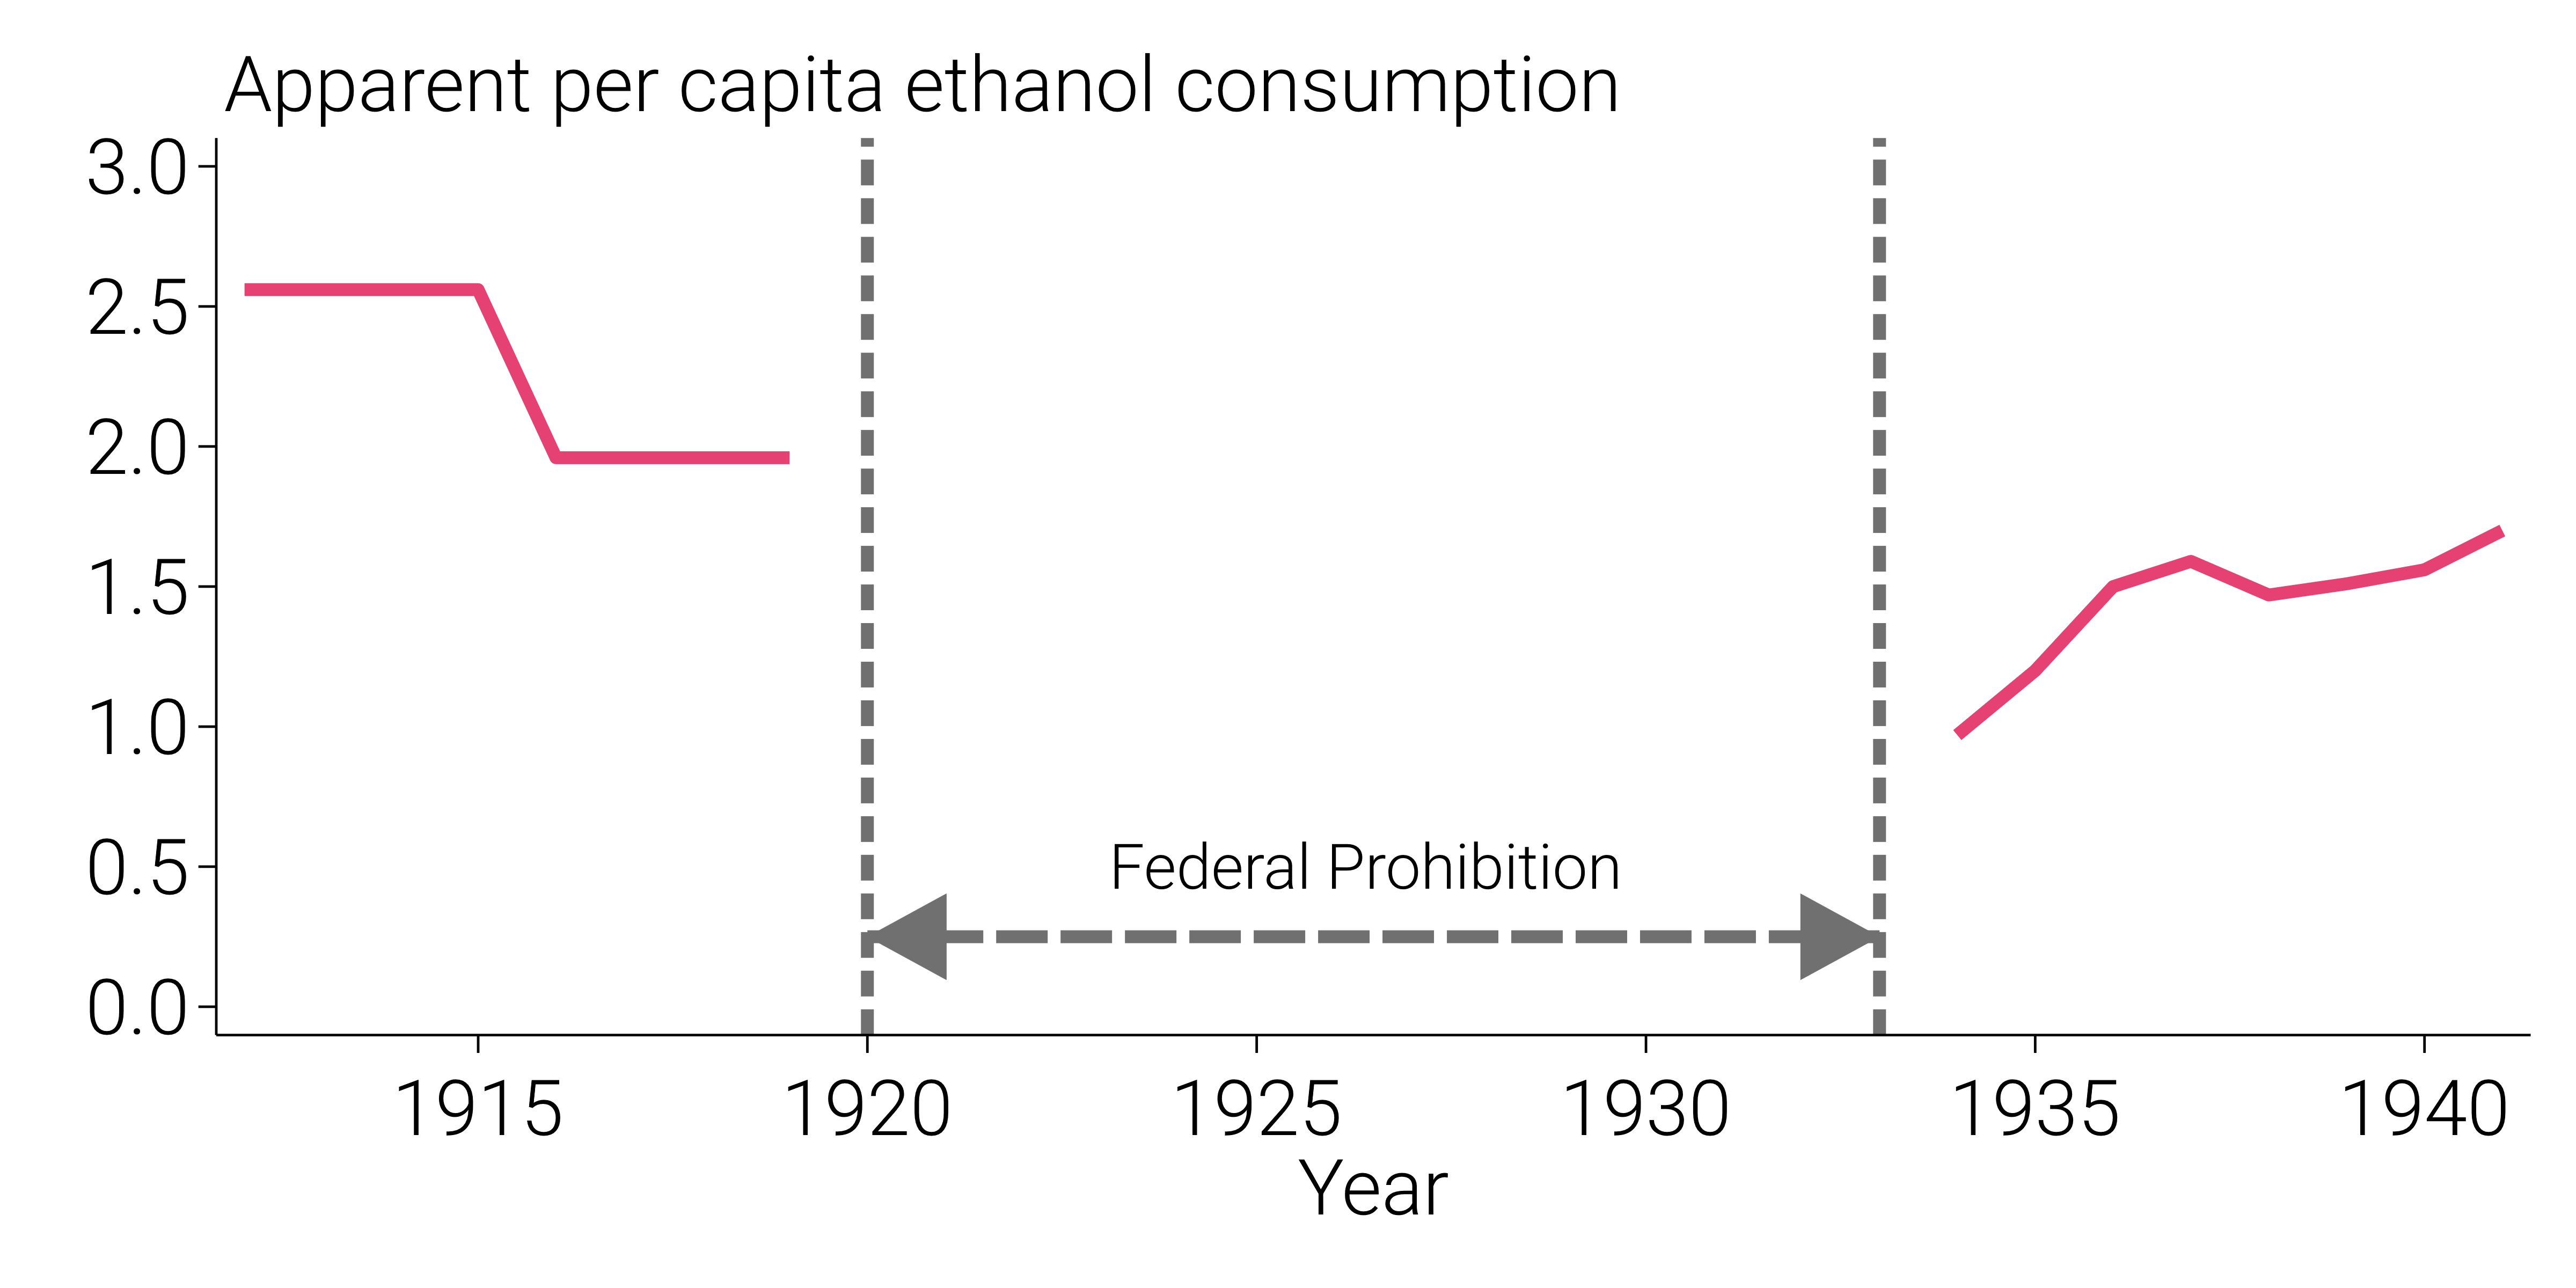
\includegraphics[width=1.0\linewidth]{../analysis/output/main/figure_1a_ethanol_consumption.png}
    \end{subfigure}
    \begin{subfigure}{0.45\linewidth}
        \centering 
        \caption[Share of US Population in Wet States]{Share of US Population in Wet States}
        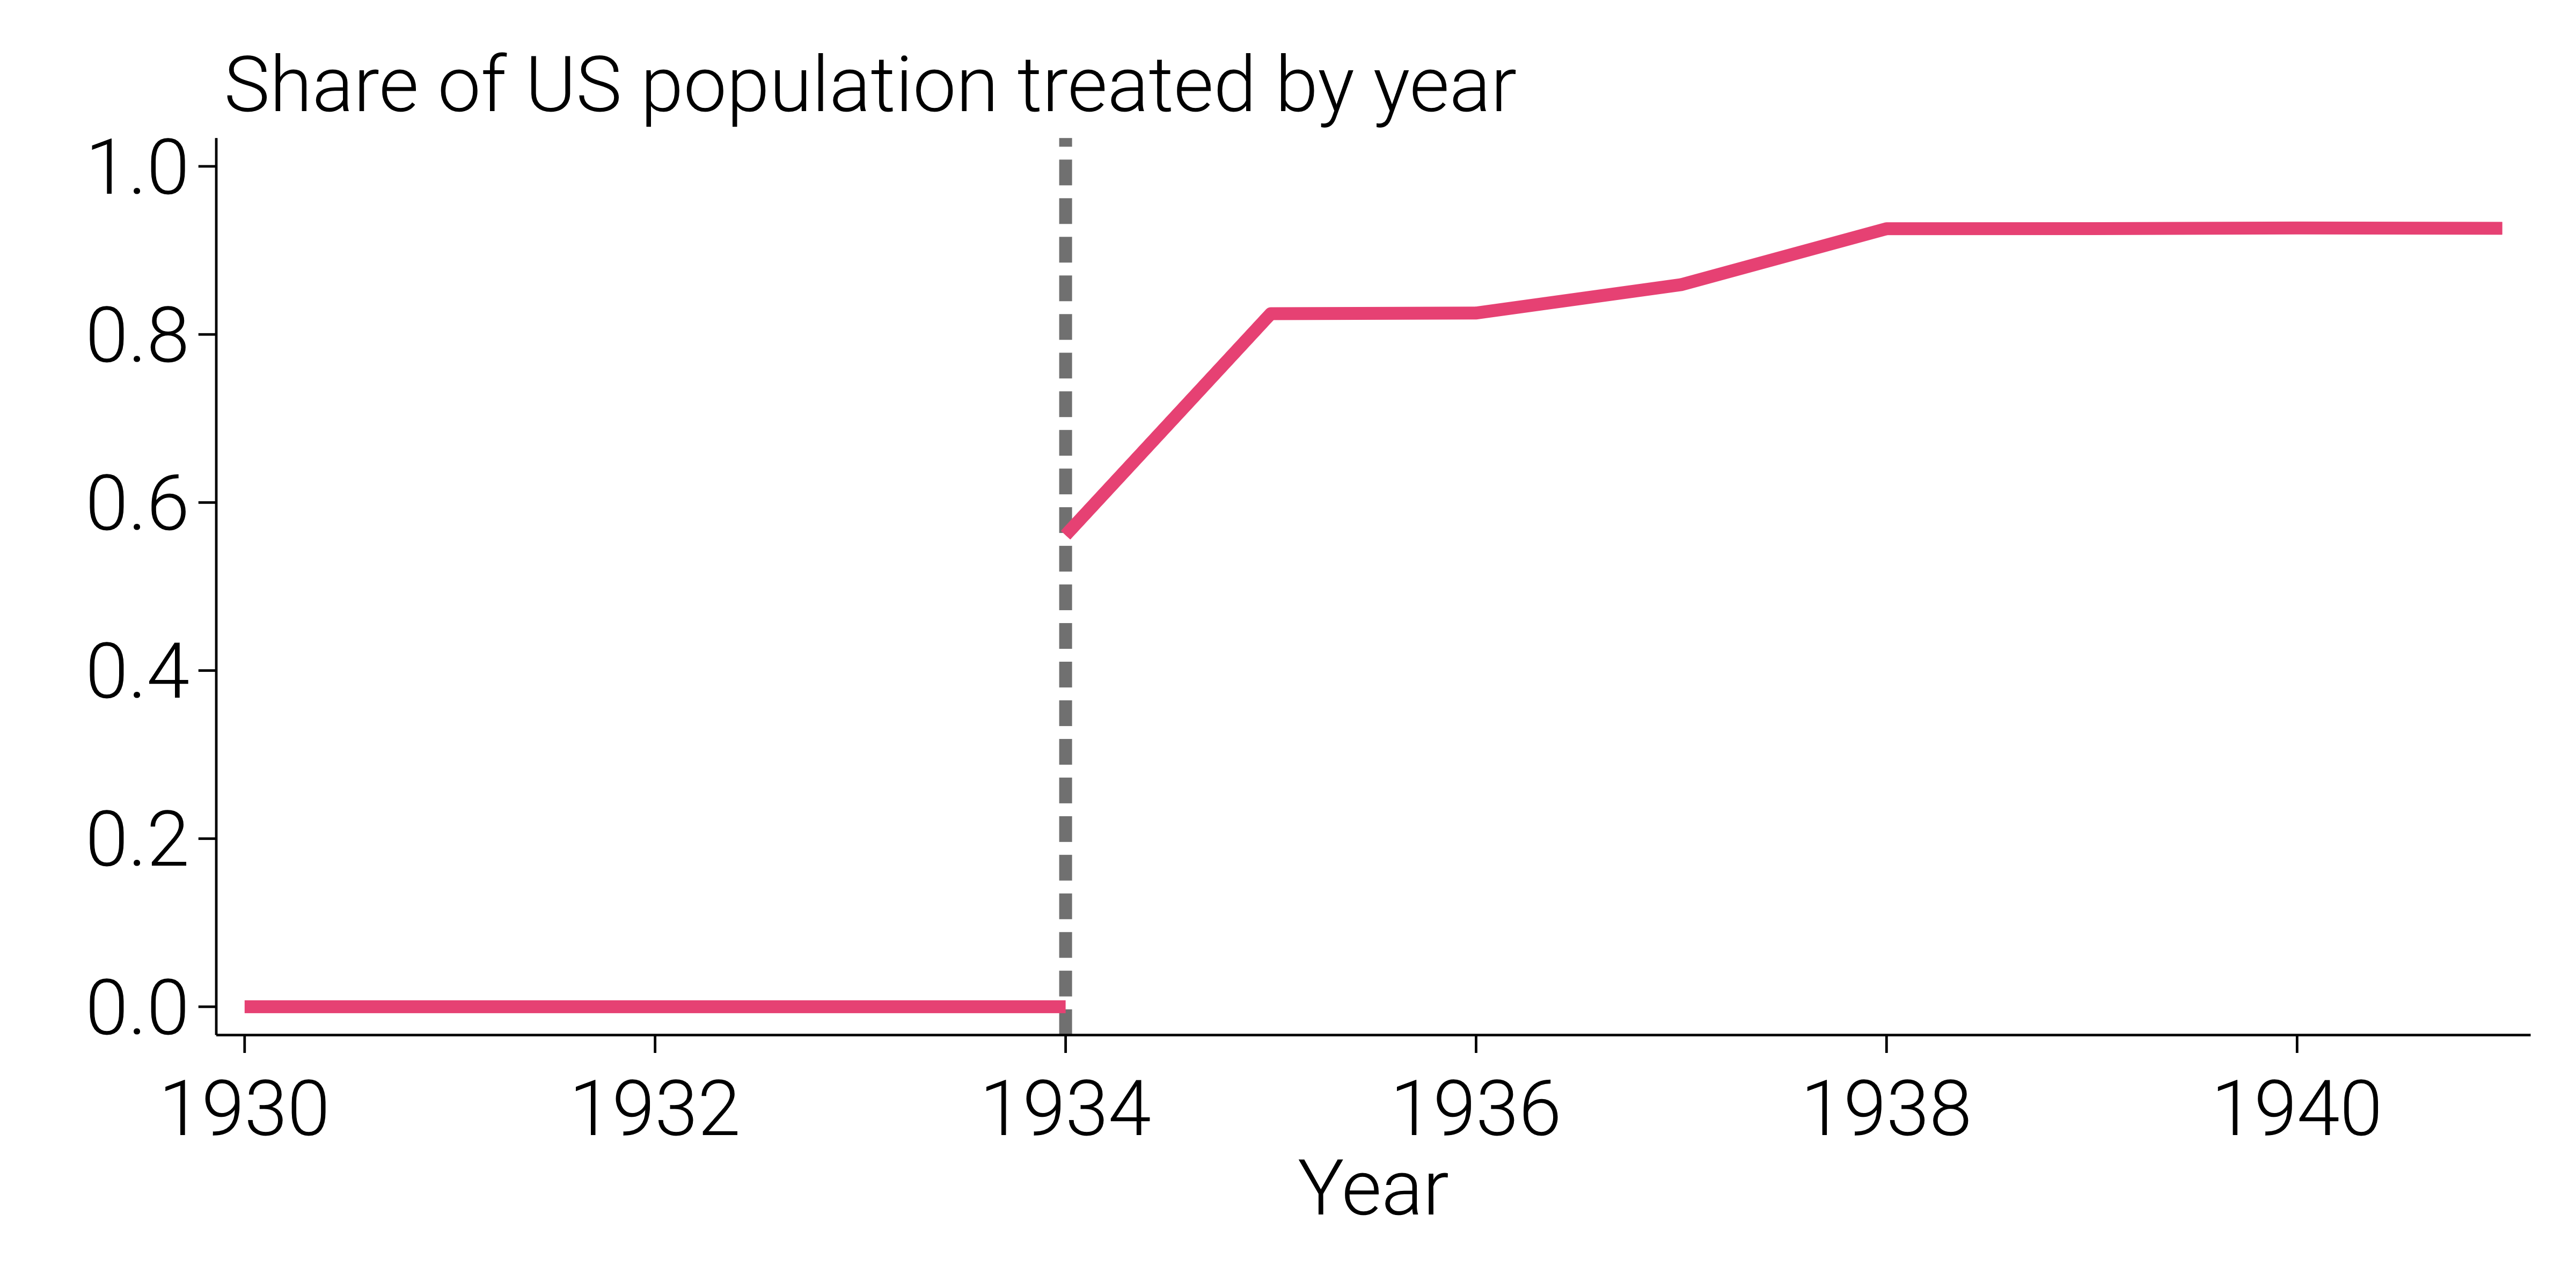
\includegraphics[width=1.0\linewidth]{../analysis/output/main/figure_1b_shr_pop_treated.png}
    \end{subfigure}
    \begin{subfigure}{0.45\linewidth}
        \centering 
        \caption[State-Level Variation in Treatment Timing]{State-Level Variation in Treatment Timing}        
        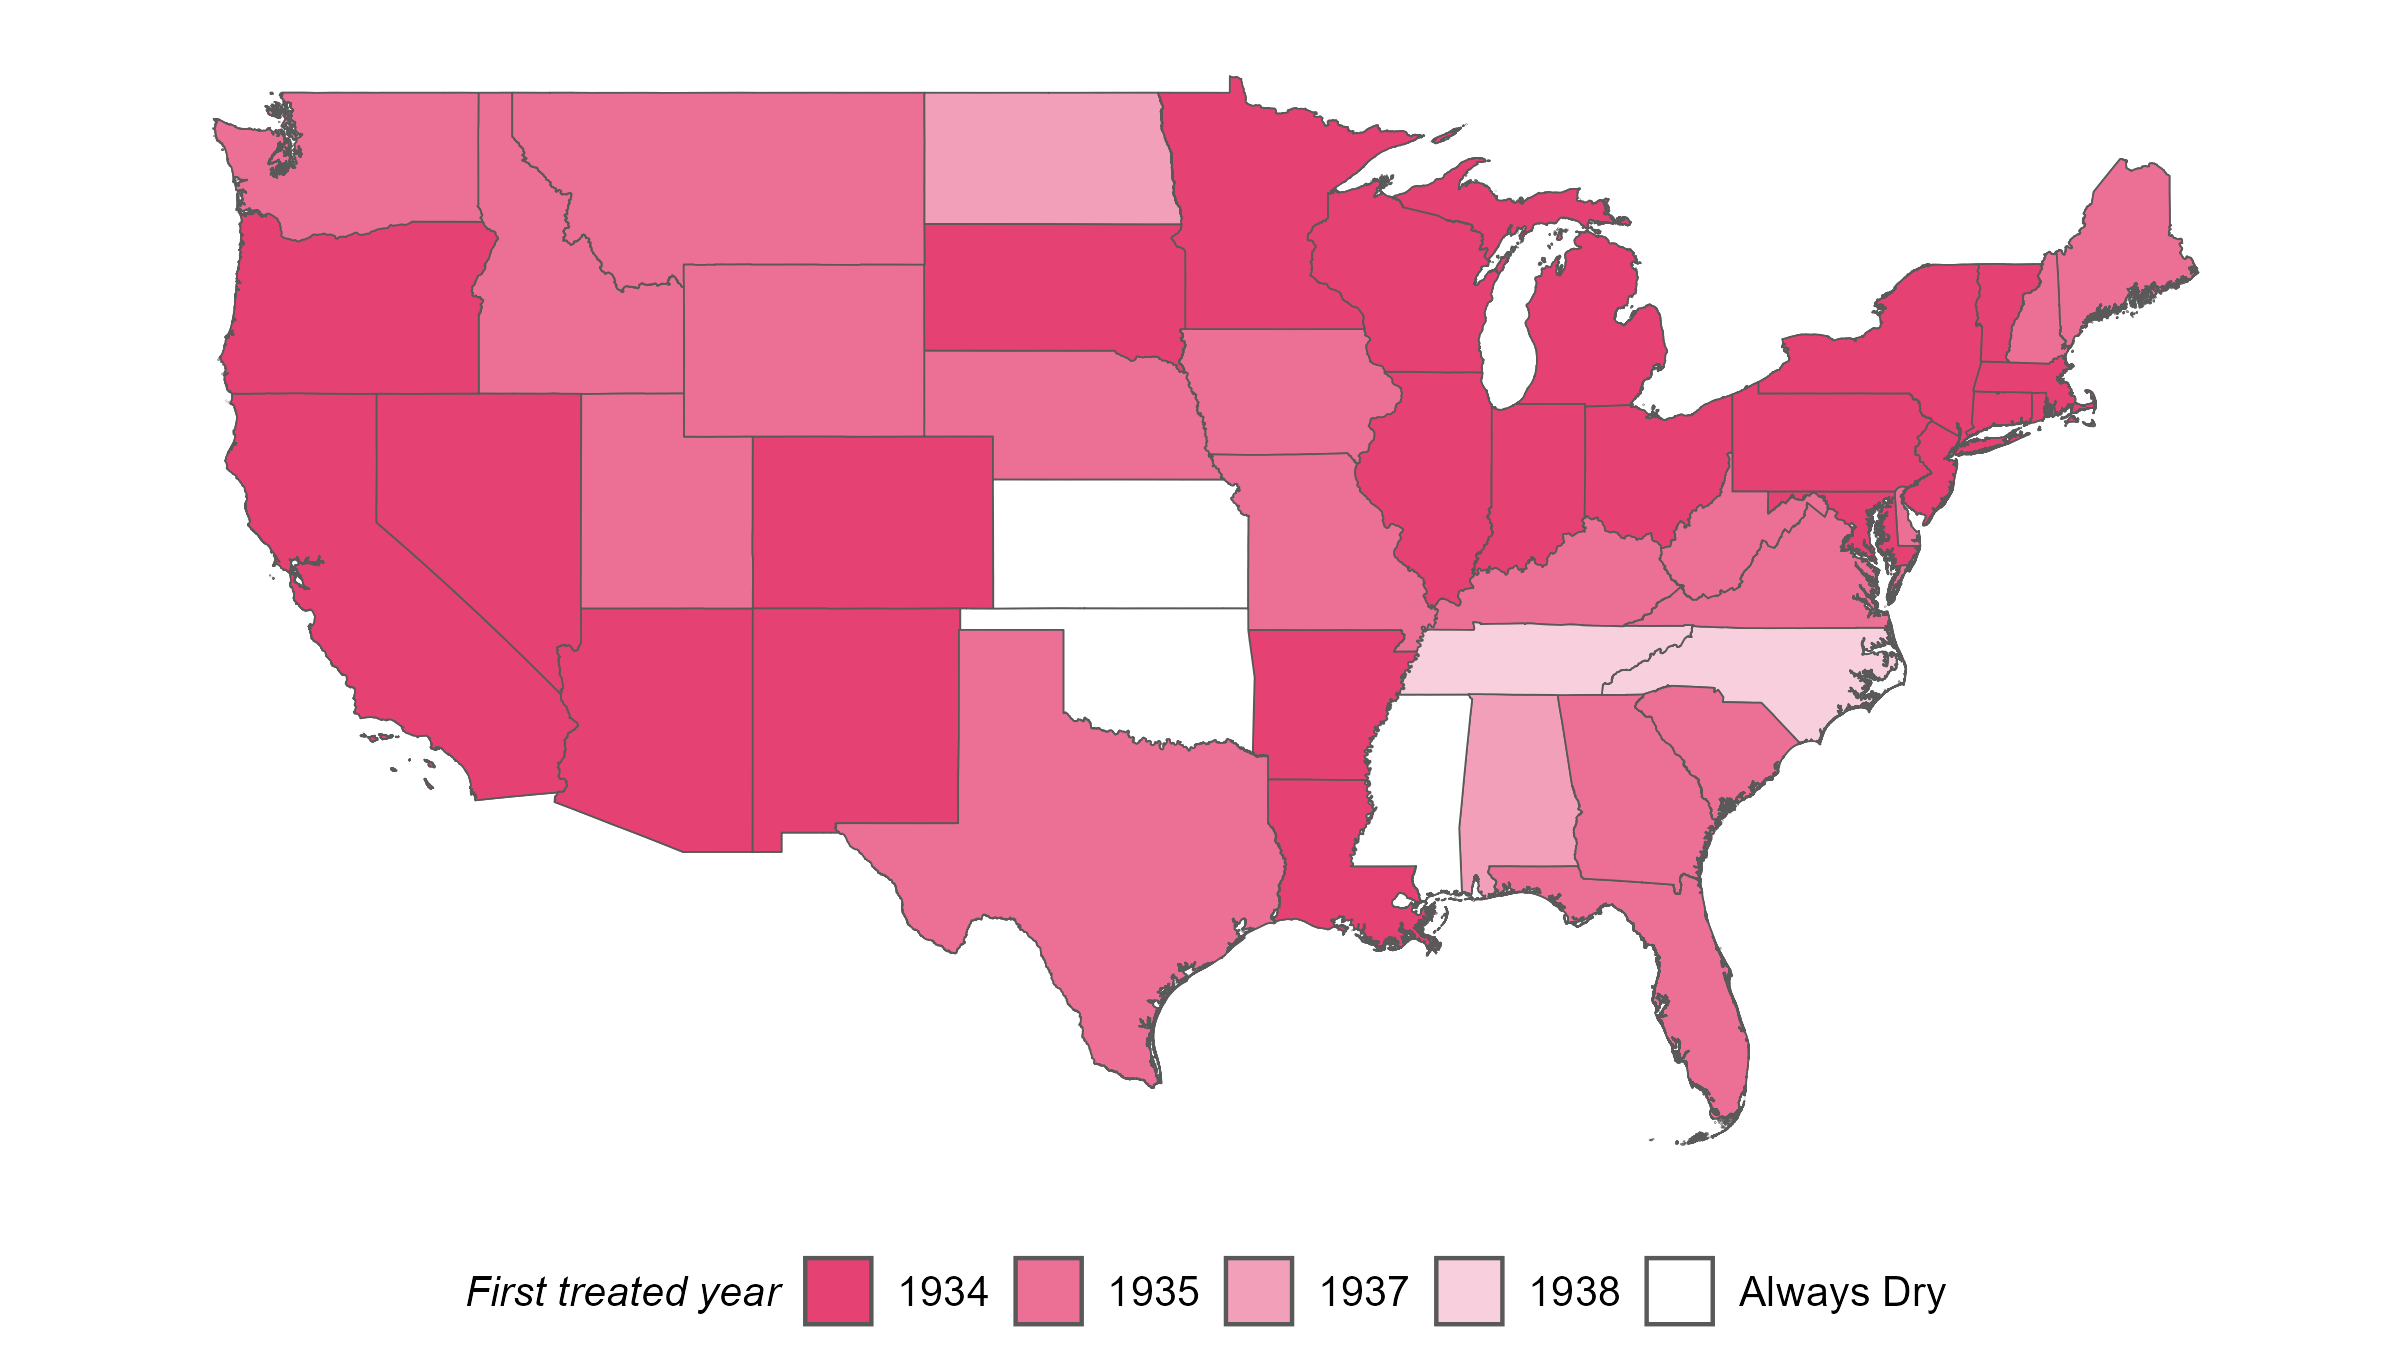
\includegraphics[width=1.0\linewidth]{../analysis/output/main/figure_1c_wet_map.png}
    \end{subfigure}
    \begin{subfigure}{0.45\linewidth}
        \centering 
        \caption[Age-Adjusted Mortality]{Age-Adjusted Mortality}        
        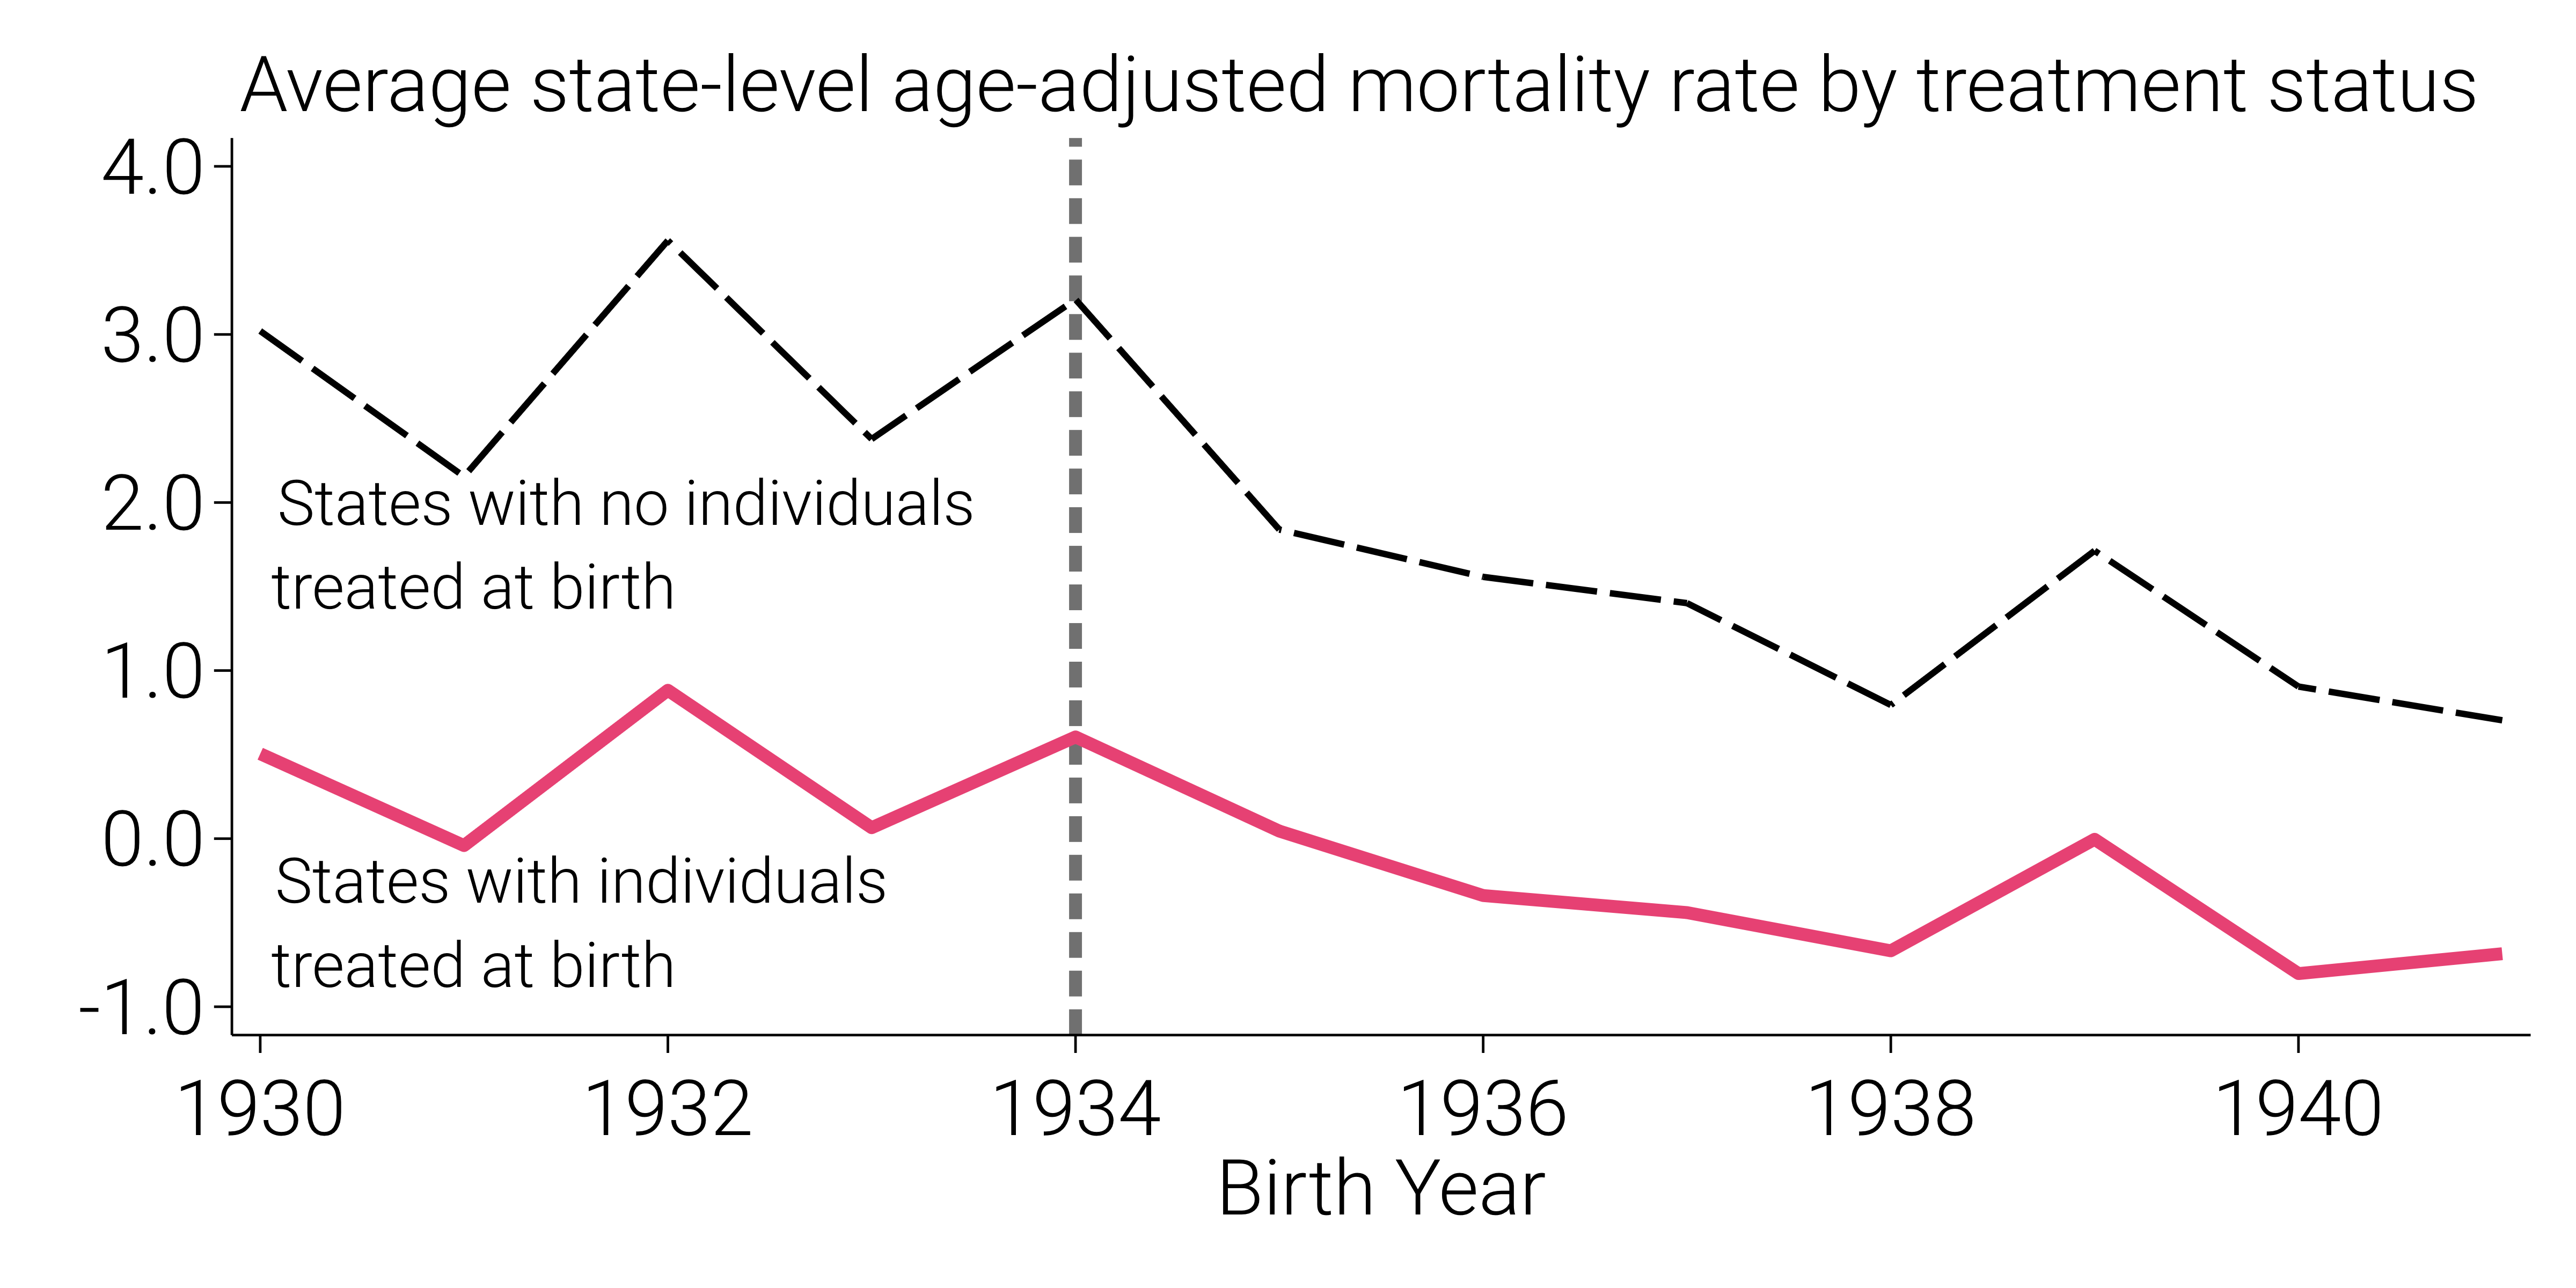
\includegraphics[width=1.0\linewidth]{../analysis/output/main/figure_1d_resid_death_by_birthyear.png}
    \end{subfigure}
    \Fnote{
        Panel A depicts apparent alcohol consumption on a per capita basis which is derived from alcoholic beverage sales data and is measured in gallons of pure ethanol. 
        Source: \citeMain{lavallee_apparent_2011}. 
        Panel B displays the prohibition status of all US states using population weights derived from the US Census to construct the share of the US population in wet states by year. 
        In our baseline specification, wet states are those which allow for (at least some) alcohol sales anywhere within their borders. 
        Source: \citeMain{jacks_infant_2021}. Panel C displays the initial year when a state turned wet. 
        The only states that remained ``always dry'' from 1930 to 1941 form the control group (i.e., Kansas, Mississippi, and Oklahoma). 
        Map source: \citeMain{manson_ipums_2020}. 
        Panel D plots averages of residuals from a regression of later-life mortality rates per 1,000 population on fixed effects for age at death, separately for states that ever turn wet between 1930 and 1941 (solid red line) and the three states in the control group that remained ``always dry'' (dashed black line).
    }
    \label{fig:descriptive-plots}
\end{figure}
\end{landscape}
\restoregeometry


% Figure 2 - Event study - All-cause mortality, heart disease, stroke, and cancer
\newpage 
\newgeometry{top = 0.5in, bottom = 0.5in, right = 0.5in, left = 0.5in, footskip = 0.0in}
\begin{landscape}
\begin{figure}[!ht]
    \caption[Event Studies By Cause of Death)]{Event Studies By Cause of Death}
    \centering
    \begin{subfigure}{0.49\linewidth}
        \centering 
        \caption[All-Cause Mortality]{All-Cause Mortality}        
        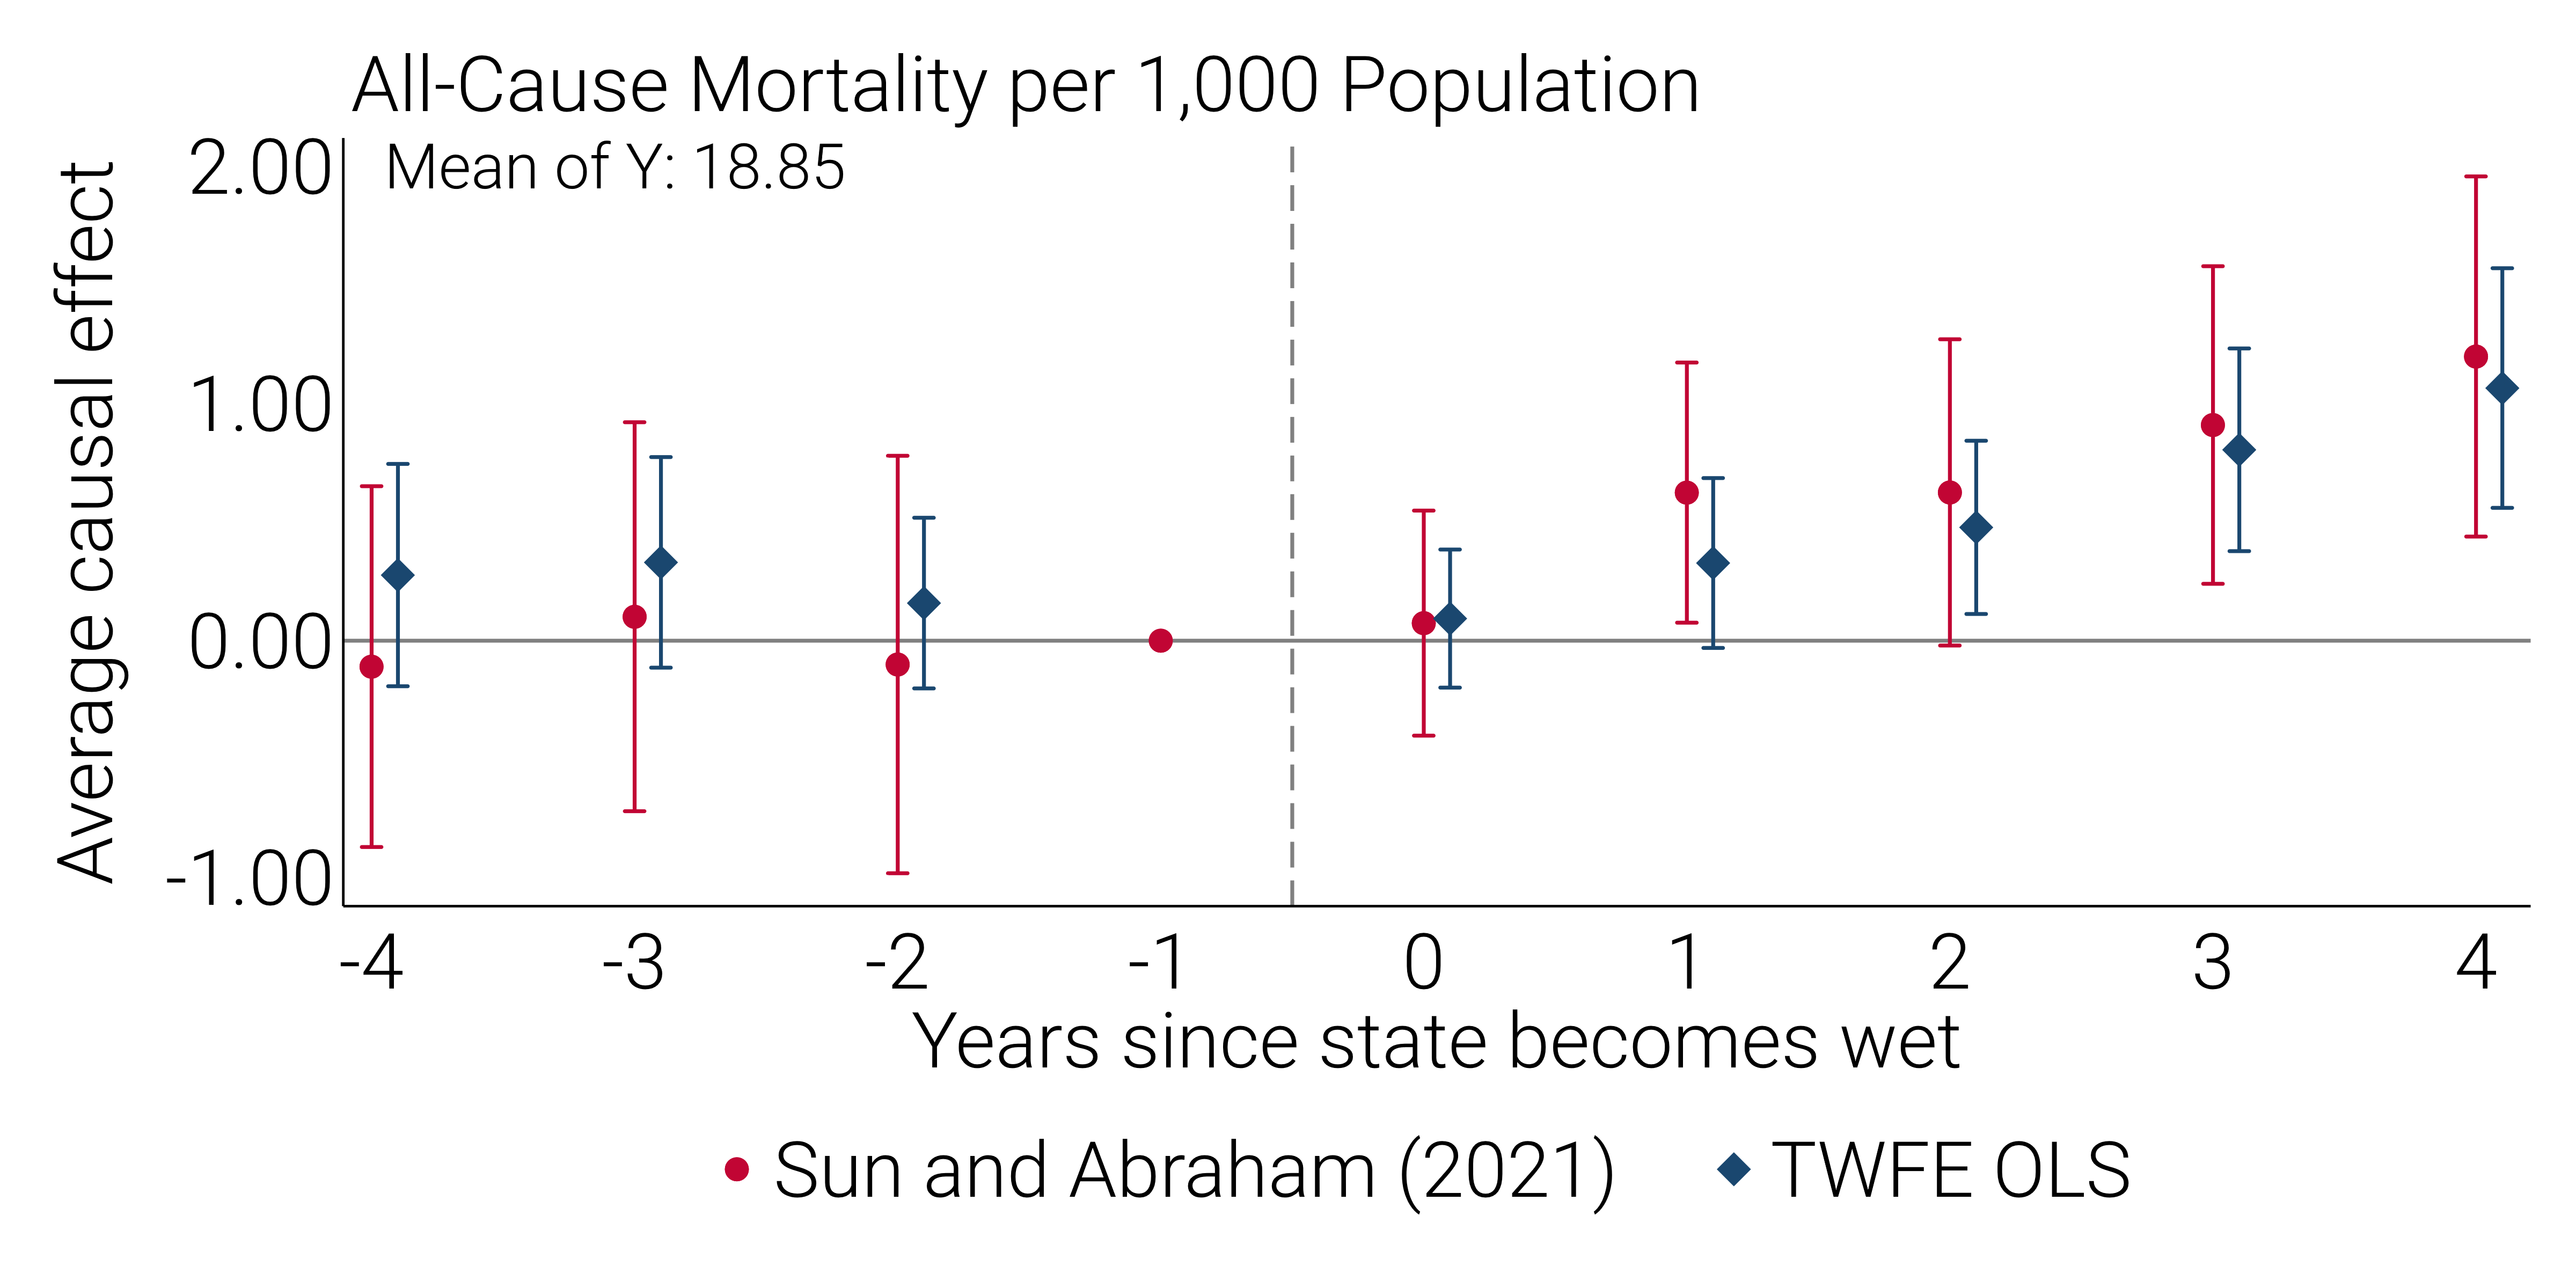
\includegraphics[width=1.0\linewidth]{../analysis/output/main/figure_2a_event_study_deaths.png}
    \end{subfigure}
    \begin{subfigure}{0.49\linewidth}
        \centering 
        \caption[Heart Disease Mortality]{Heart Disease Mortality}        
        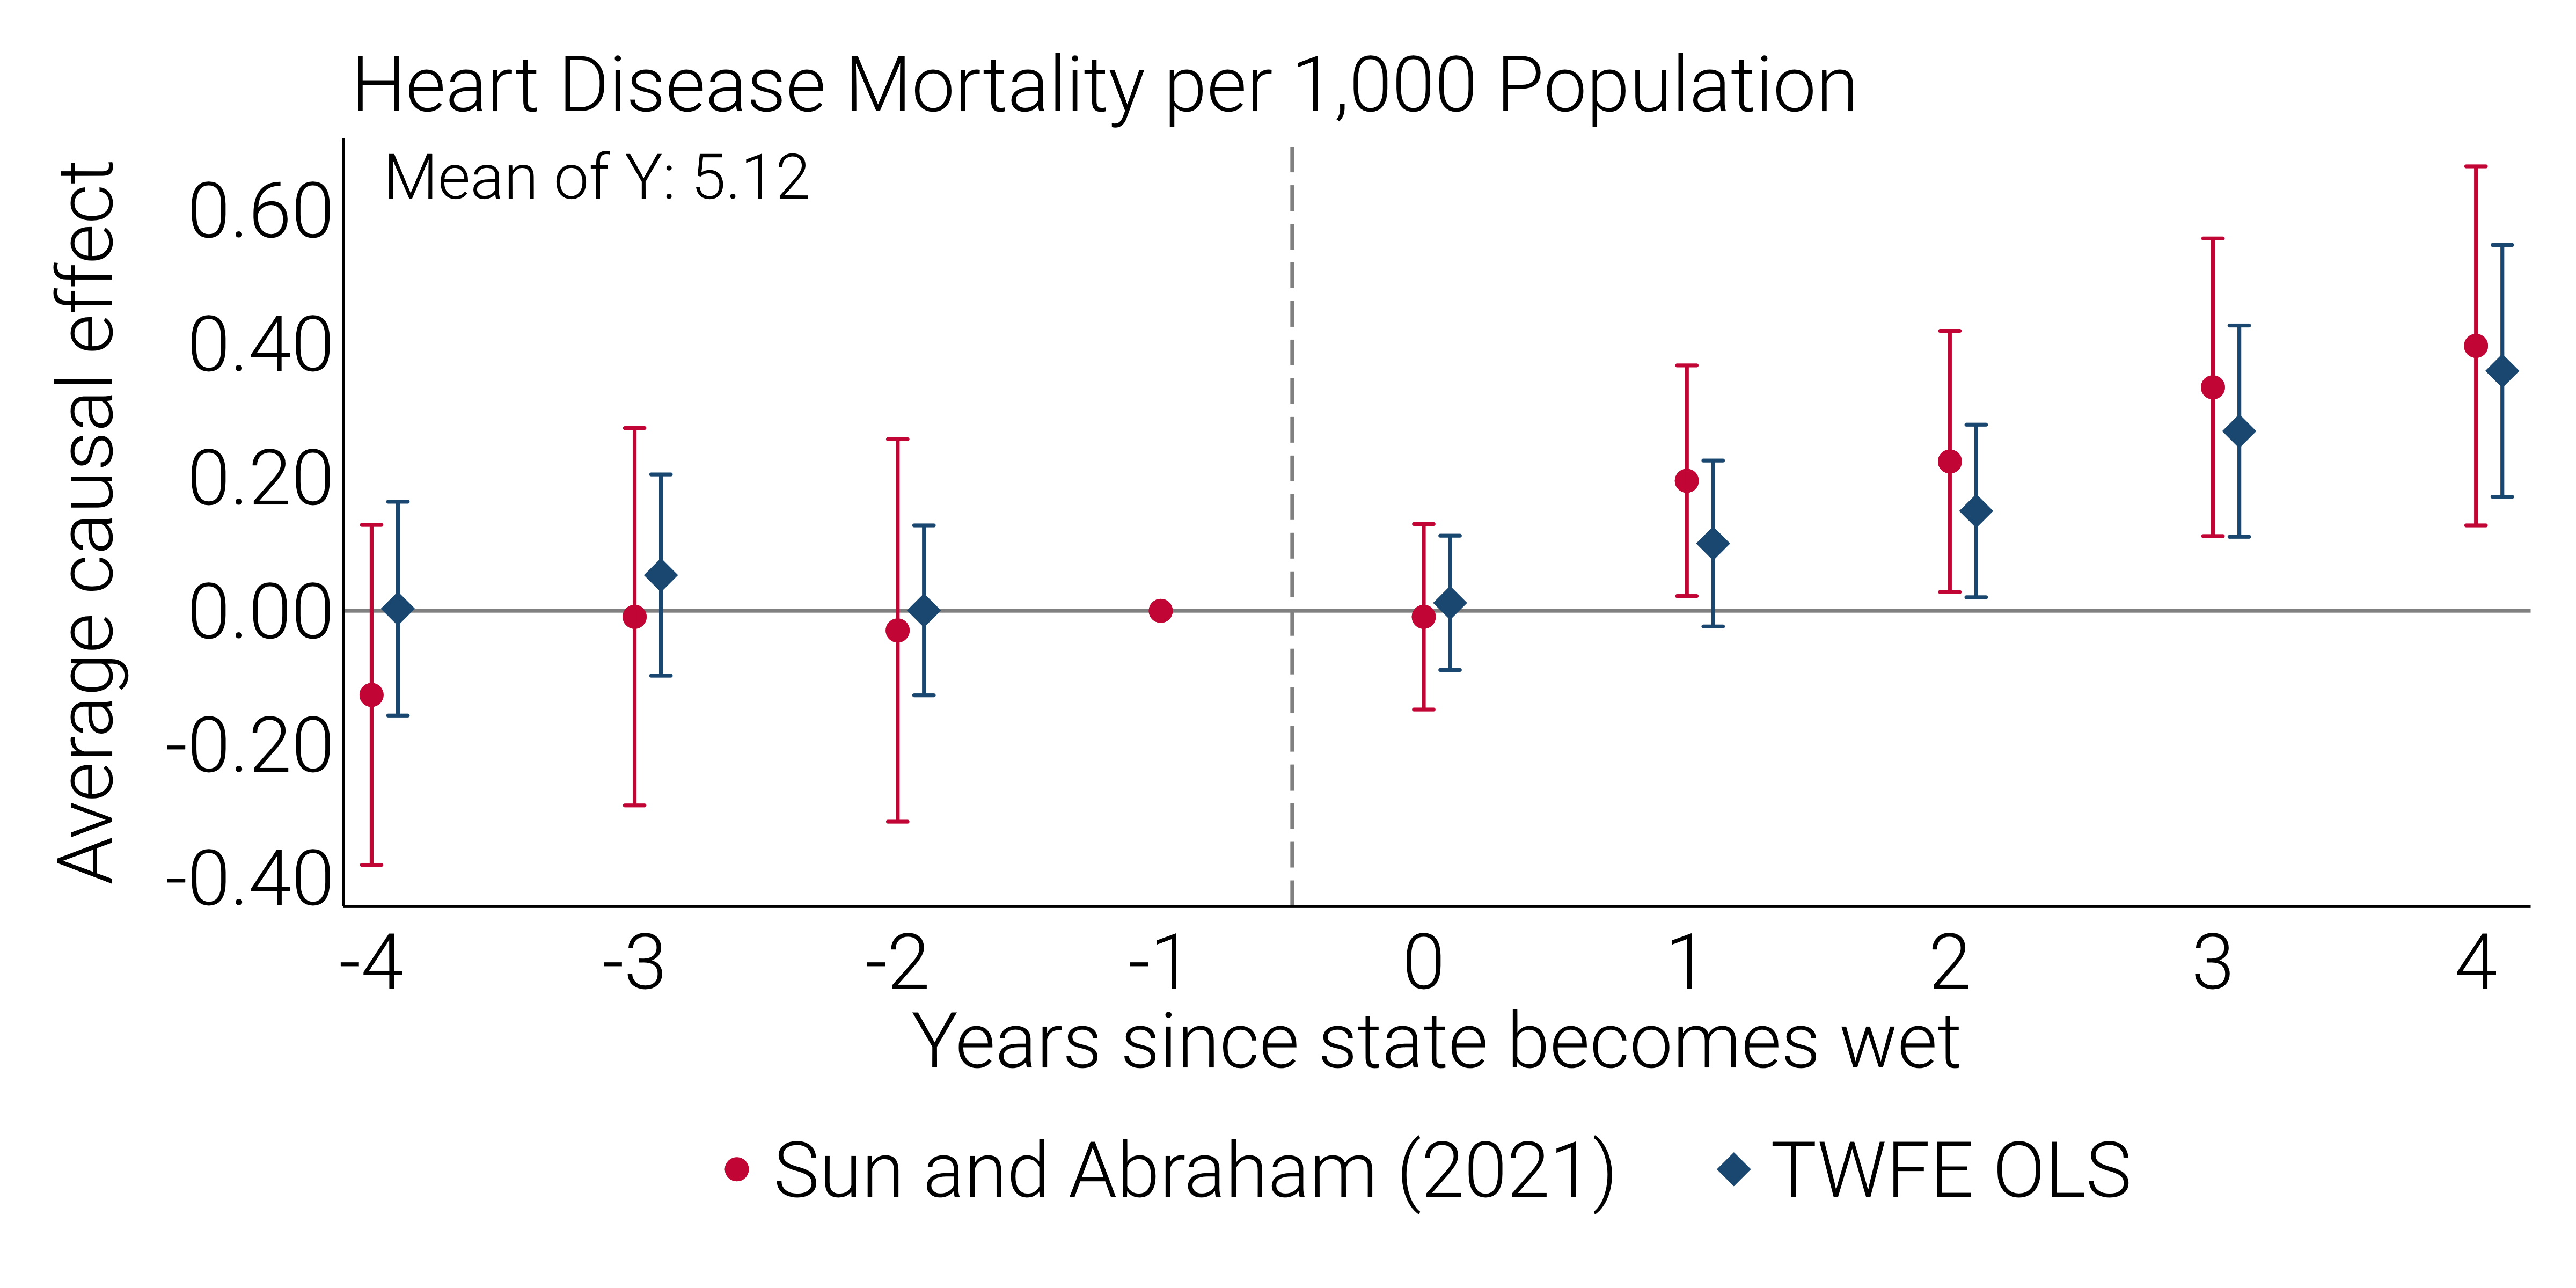
\includegraphics[width=1.0\linewidth]{../analysis/output/main/figure_2b_event_study_heart.png}
    \end{subfigure}
    \begin{subfigure}{0.49\linewidth}
        \centering 
        \caption[Stroke Mortality]{Stroke Mortality}        
        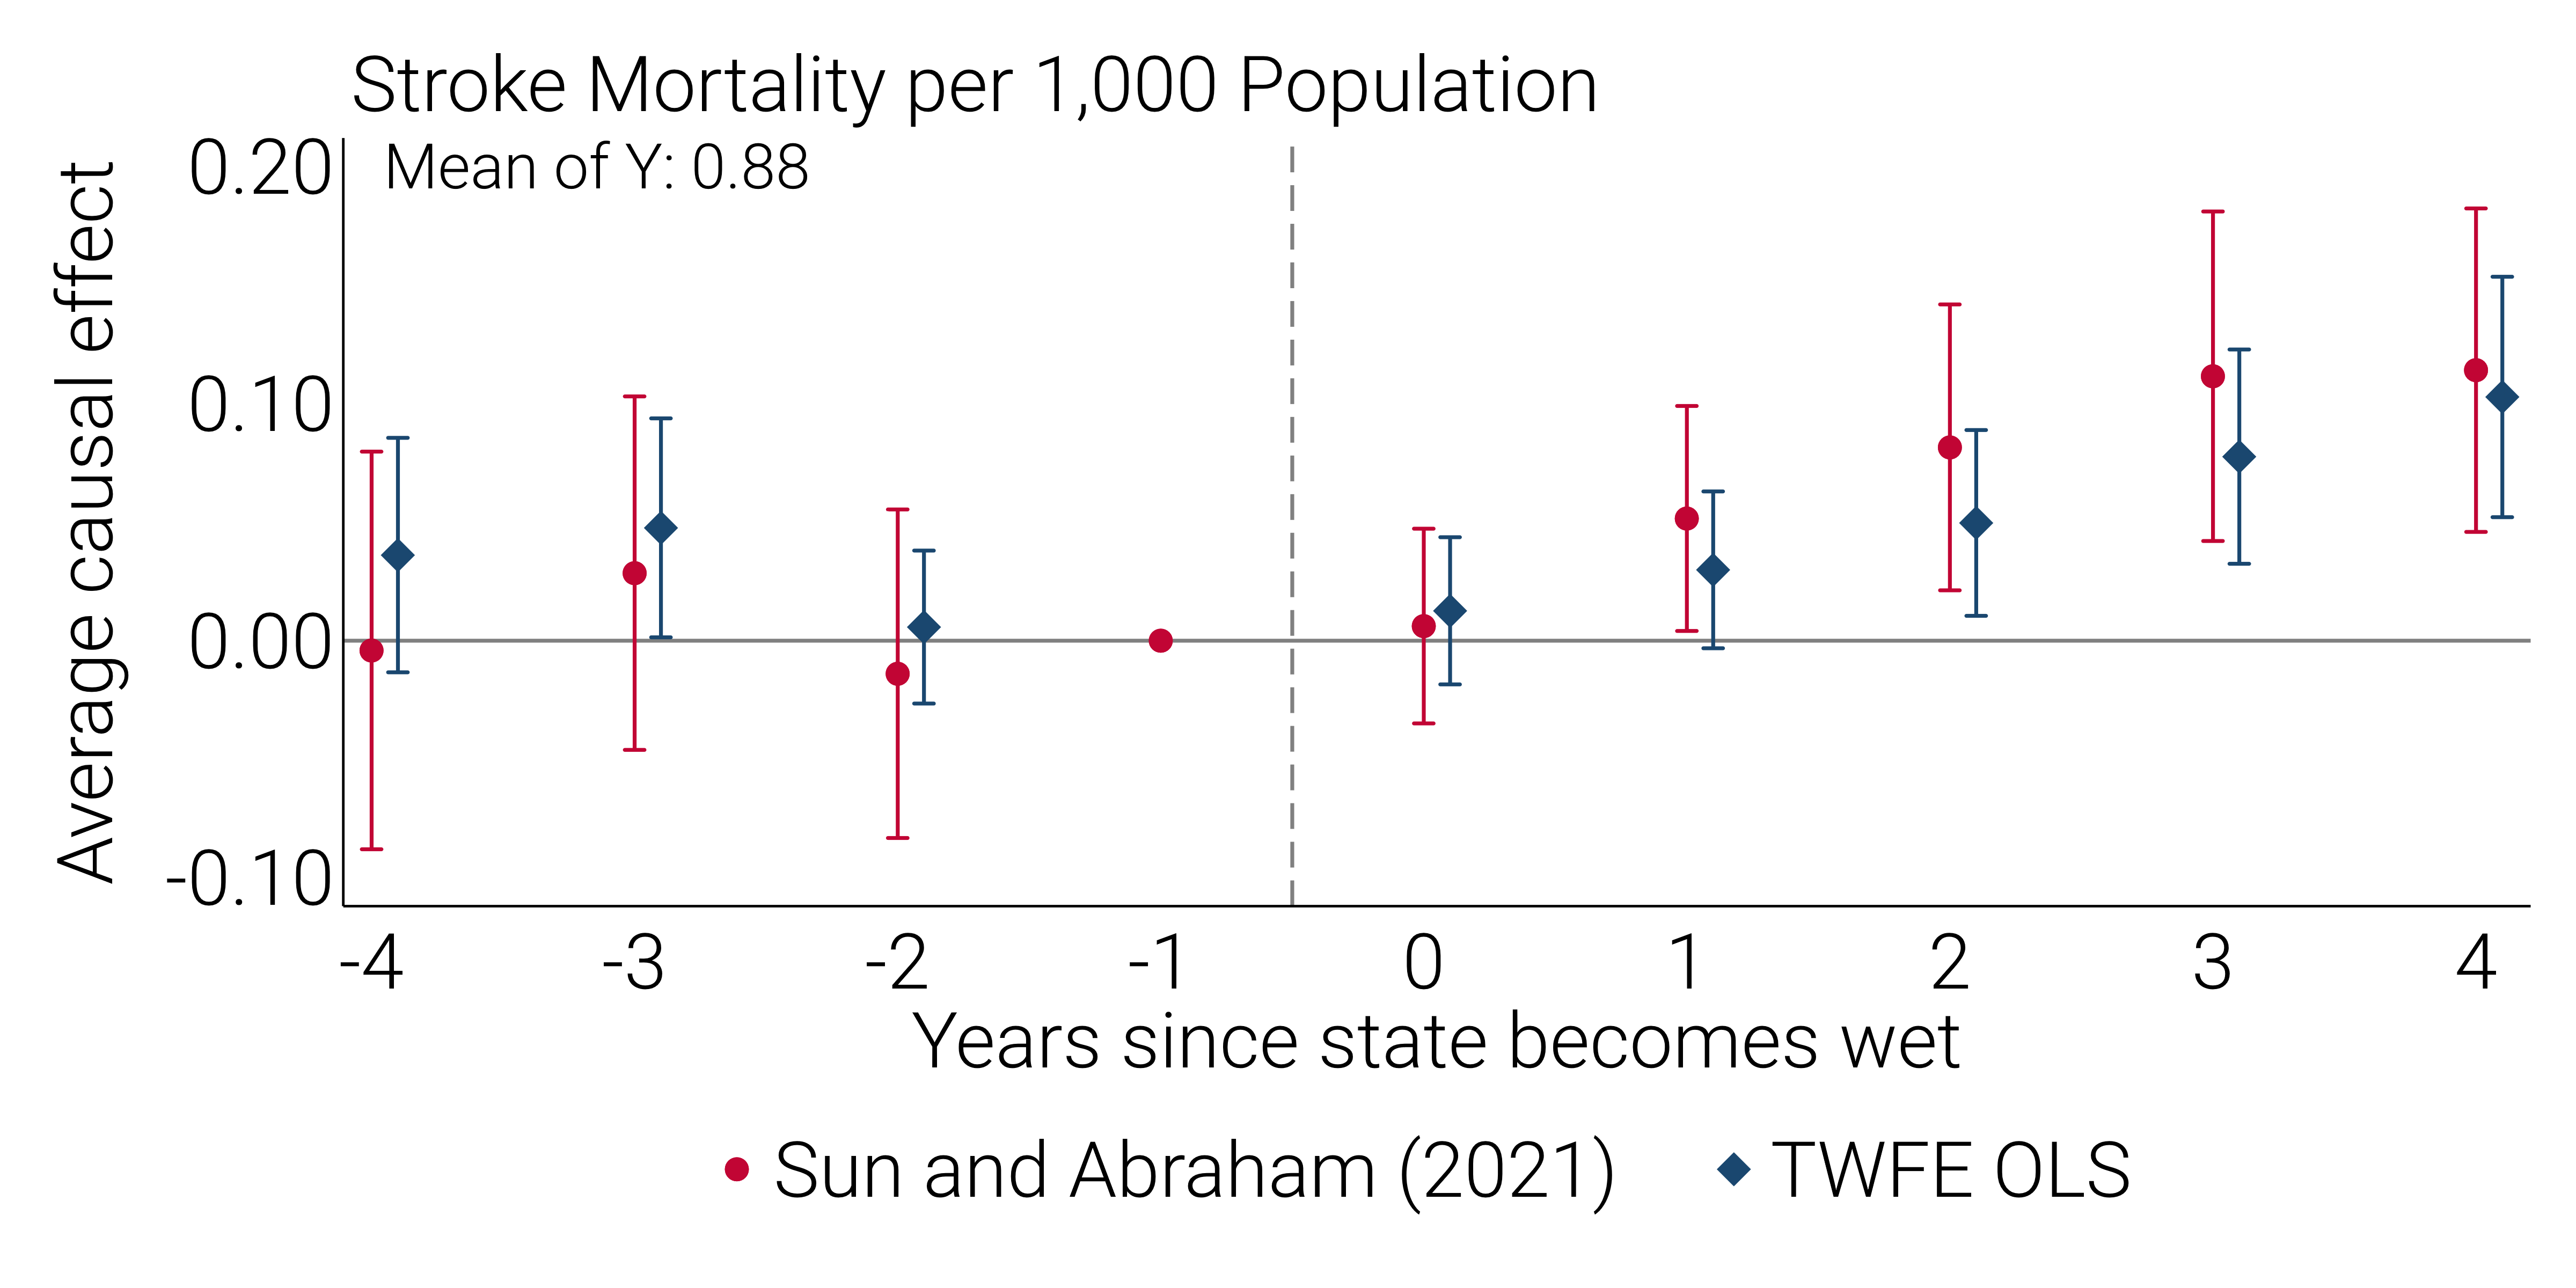
\includegraphics[width=1.0\linewidth]{../analysis/output/main/figure_2c_event_study_stroke.png}
    \end{subfigure}    
    \begin{subfigure}{0.49\linewidth}
        \centering 
        \caption[Cancer Mortality]{Cancer Mortality}        
        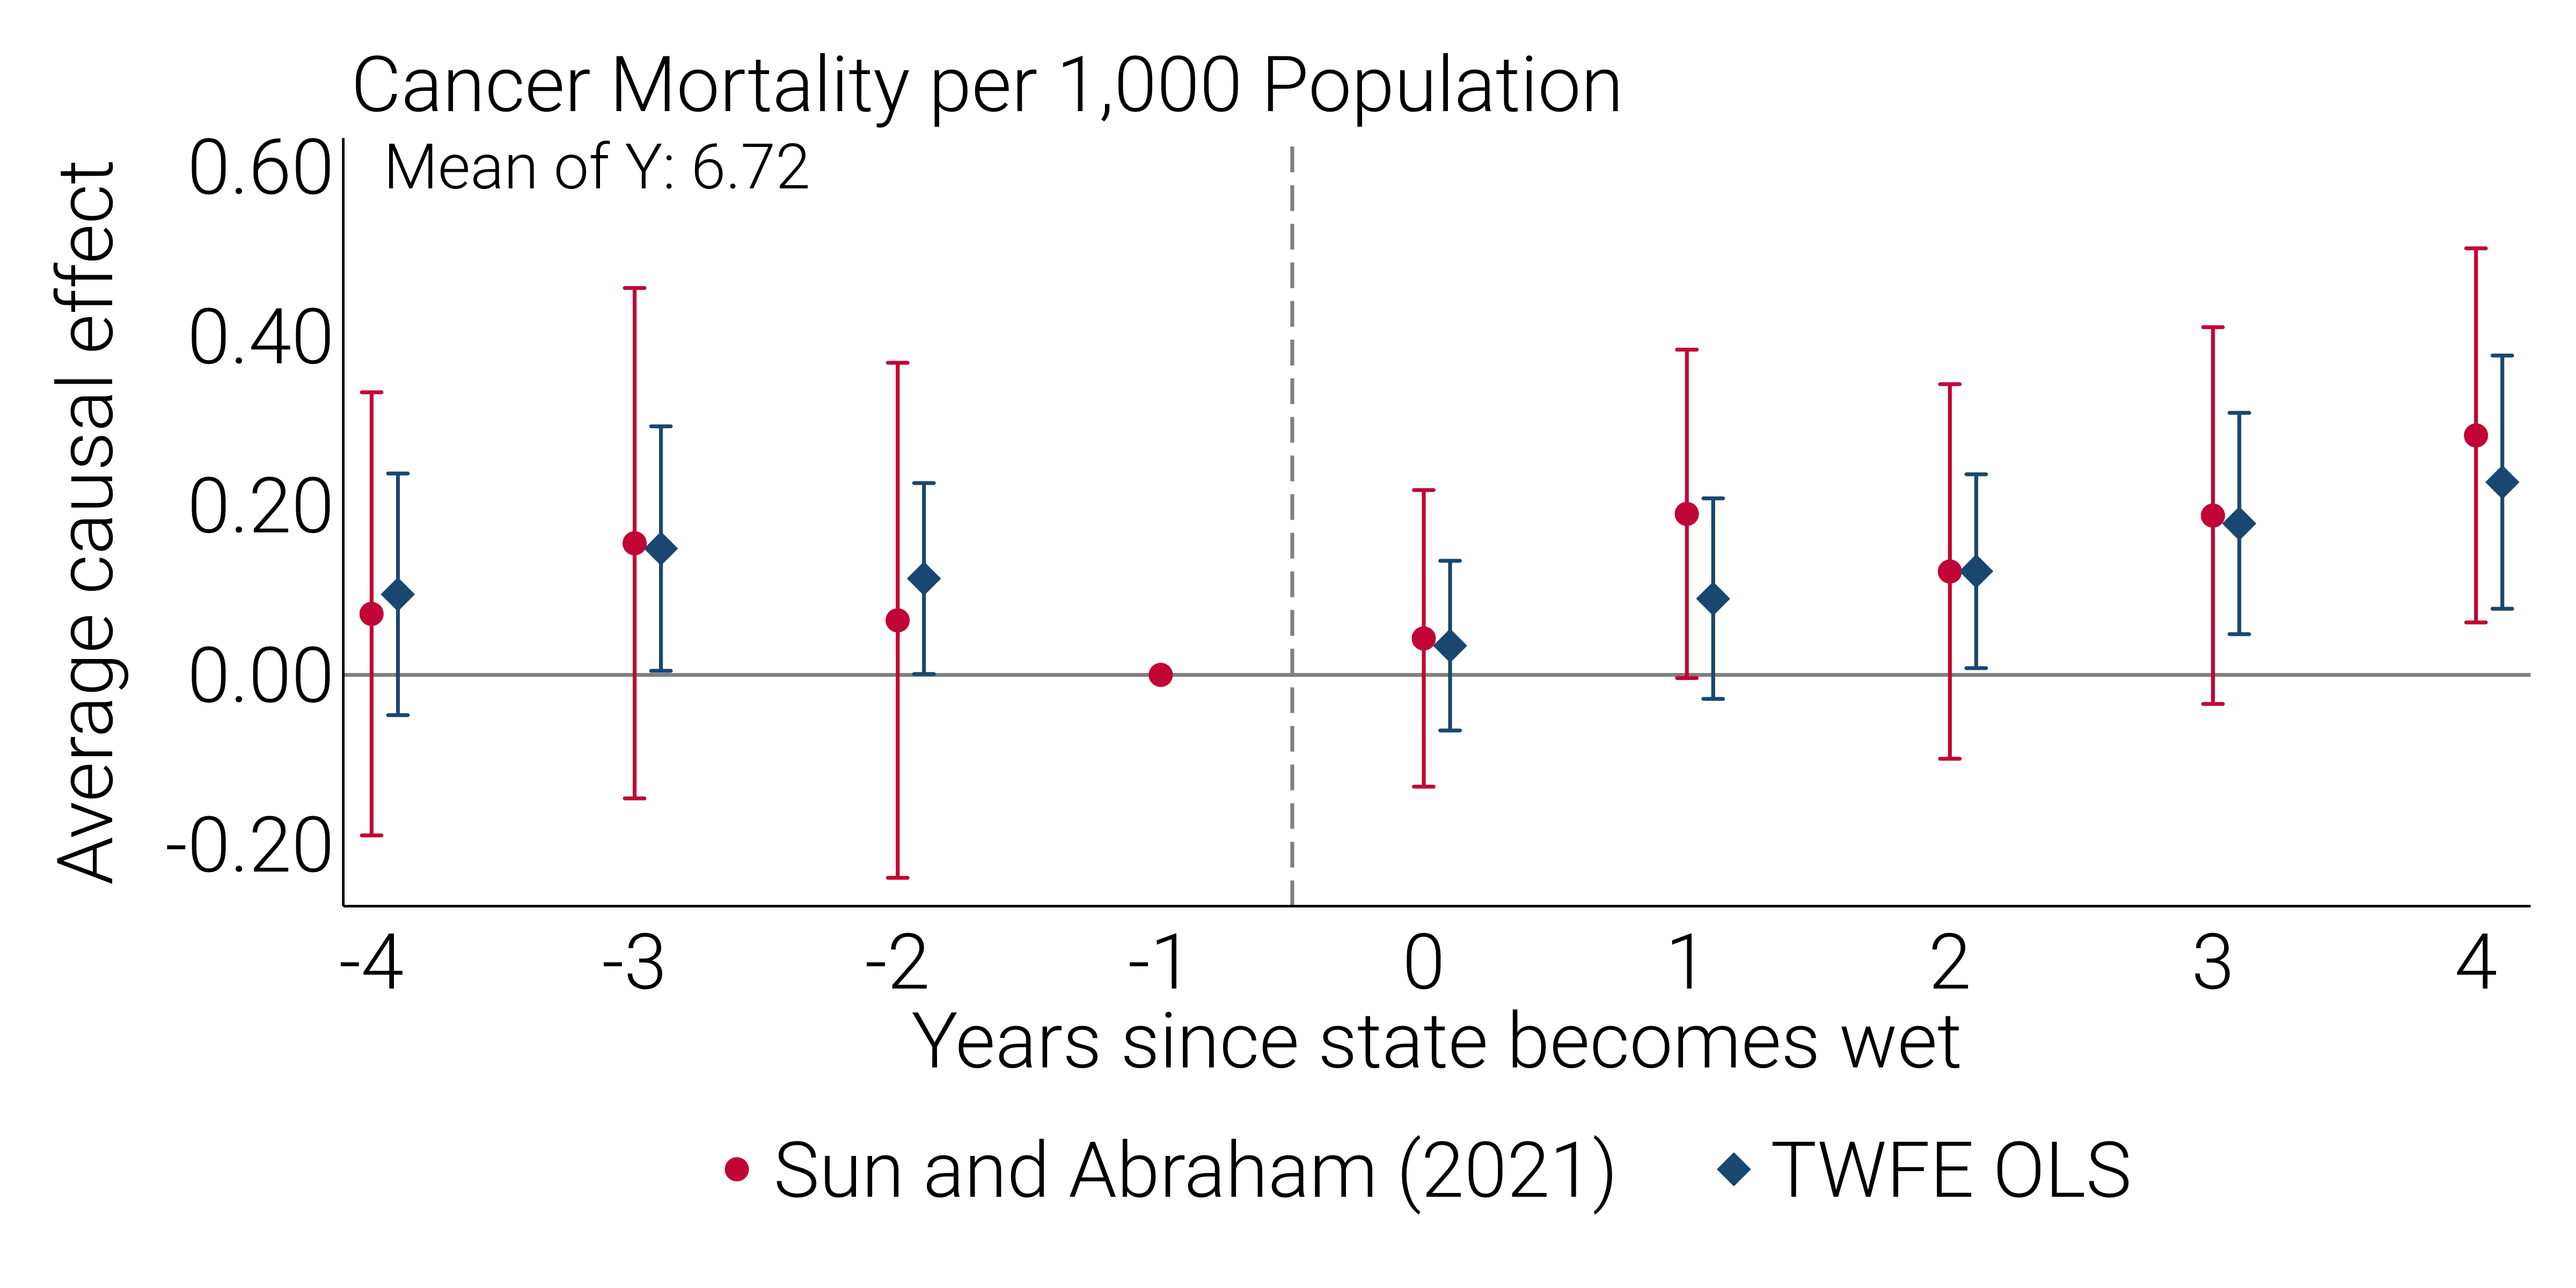
\includegraphics[width=1.0\linewidth]{../analysis/output/main/figure_2d_event_study_cancer.png}
    \end{subfigure}
    \Fnote{
        Each panel displays event studies with all-cause mortality (panel A) or cause-specific mortality per 1,000 population as the dependent variable (heart disease in panel B, stroke in panel C, and cancer in panel D). 
        The unit of observation is the annual mortality rate for a given state of birth by year of birth cohort. 
        The sample includes the 1930 to 1941 birth cohorts. 
        The ``Mean of Y'' is the sample mean of the dependent variable for pre-treatment (1930-1933) birth cohorts in not-yet-treated states.  
        Mortality is observed between 1990 and 2004. 
        Each panel shows event studies based on two estimation methods: \citeMain{sun_estimating_2021} and TWFE OLS. 
        The coefficients for event-time periods $l = -8$ to $l = -5$ and $l = 5$ to $l = 7$ are omitted for clarity and due to compositional changes in the set of treated states. 
        All specifications include the year of birth by death year and state of birth by death year fixed effects. 
        Observations are weighted by the surviving cohort size for each state of birth by year of birth by death year cell. 
        Standard errors are clustered at the state of birth by year of birth level.
    }
    \label{fig:event-study-cause-of-death}
\end{figure}
\end{landscape}
\restoregeometry

\newpage
\FloatBarrier

\section[Tables]{Tables\label{sec:Tables}}

% Table 1. Robustness of aggregate event study estimates 
\begin{table}[!ht]\centering
  \begin{adjustbox}{width=1.0\textwidth}
  \centering
    \begin{threeparttable}
     \caption{Aggregate Event Study Estimates for All-Cause Mortality}
     \estauto{../analysis/output/main/table_1_aggregate_event_study_regressions.tex}{6}{S[table-format=2.3,table-column-width=20mm, table-alignment = center]}
      \label{tab:es-main-specs}
      \Fignote{
            The unit of observation is the annual mortality rate for a given state of birth by year of birth cohort. 
            The sample includes the 1930 to 1941 birth cohorts. 
            The ``Mean of Y'' is the sample mean of the dependent variable for pre-treatment (1930-1933) birth cohorts in not-yet-treated states. 
            Mortality is observed between 1990 and 2004. 
            The dependent variable is the number of deaths per 1,000 population. 
            Each coefficient is the average of the \citeMain{sun_estimating_2021} event study coefficients from $l = 0$ to $l = 4$ and represents the average change in the later-life all-cause mortality rate attributable to in utero exposure to the first five years of federal prohibition's repeal. 
            In columns 1 to 3, observations are treated (i.e., the indicator for wet status equals one) if at least some alcohol sales were allowed anywhere within the state of birth in the year of birth. 
            The specification for Column 1 corresponds to the event study in Panel A of Figure~\ref{fig:event-study-cause-of-death} where all-cause mortality rates are a function of state of birth by death year and year of birth by death year fixed effects. 
            Column 2 includes control variables for the log of per capita New Deal spending and the log of per capita real disposable personal income at the state level. 
            Columns 3 through 6 also retain these controls. Column 3 uses the last treated states (North Carolina and Tennessee) as the control group, thereby dropping observations for the 1938 to 1941 birth cohorts. 
            In Column 4, a state is considered to be treated only if the entire state turns wet via statewide legislation while in Column 5 a state is considered to be treated if at least 50\% of the population resided in counties that allowed for legal alcohol sales. 
            Column 6 reverts to the original definition of the treatment variable but uses standard errors clustered at the state of birth level. 
            In all specifications, observations are weighted by the surviving cohort size for each state of birth by year of birth by death year cell. 
            Standard errors are clustered at the state of birth by year of birth level in Columns 1 to 5. 
            Standard errors are in parentheses; t-statistics reported below standard errors in brackets.
        }
    \end{threeparttable}
   \end{adjustbox}
\end{table}

% Table 2: By Cause of Death
\begin{table}[!ht]\centering
  \begin{adjustbox}{width=1.0\textwidth}
  \centering
    \begin{threeparttable}
     \caption{Aggregate Event Study Estimates for Cause-Specific Mortality}
     \estauto{../analysis/output/main/table_2_cause_of_death.tex}{5}{S[table-format=2.3,table-column-width=20mm, table-alignment = center]}
      \label{tab:did-by-cause-of-death}
      \Fignote{
            The unit of observation is the annual mortality rate for a given state of birth by year of birth cohort. 
            The sample includes the 1930 to 1941 birth cohorts. 
            The ``Mean of Y'' is the sample mean of the dependent variable for pre-treatment (1930-1933) birth cohorts in not-yet-treated states. 
            Mortality is observed between 1990 and 2004. 
            The dependent variable is the number of all-cause deaths per 1,000 population (Column 1) or the number of cause-specific deaths from heart disease (Column 2), stroke (Column 3),  cancer (Column 4), or motor vehicle accidents (Column 5) per 1,000 population. 
            Each coefficient is the average of the \citeMain{sun_estimating_2021} event study coefficients from $l = 0$ to $l = 4$ and represents the average change in the later-life all-cause mortality rate attributable to in utero exposure to the first five years of federal prohibition’s repeal. 
            In all columns, observations are treated (i.e., the indicator for wet status equals one) if at least some alcohol sales were allowed anywhere within the state of birth in the year of birth. 
            In all specifications, mortality rates are a function of the state of birth by death year and year of birth by death year fixed effects and control for the log of per capita New Deal spending and the log of per capita real disposable personal income at the state level. 
            Observations are weighted by the surviving cohort size for each state of birth by year of birth by death year cell. 
            All standard errors are clustered at the state of birth by year of birth level. 
            Standard errors are in parentheses; t-statistics reported below standard errors are in brackets. 
            See Table~\ref{tab:icd-crosswalk} in Appendix~\ref{sec:additional-tab-fig} for the crosswalk of ICD9 and ICD10 codes used to construct cause-specific mortality rates.
        }
    \end{threeparttable}
   \end{adjustbox}
\end{table}

% Table 3: Heterogeneity by Race and Gender
\newgeometry{footskip = 0in}
\begin{table}[!ht]\centering
  \begin{adjustbox}{width=1.0\textwidth}
  \centering
    \begin{threeparttable}
     \caption{Aggregate Event Study Estimates for Heterogeneity by Sex and Race}
     \estauto{../analysis/output/main/table_3_heterogeneity.tex}{4}{S[table-format=2.3,table-column-width=20mm, table-alignment = center]}
      \label{tab:did-heterogeneity-gender-race}
      \Fignote{
            The unit of observation is the annual mortality rate for a given state of birth by year of birth cohort. 
            The sample includes the 1930 to 1941 birth cohorts. 
            The ``Mean of Y'' is the sample mean of the dependent variable for pre-treatment (1930-1933) birth cohorts in not-yet-treated states. 
            Mortality is observed between 1990 and 2004. 
            The dependent variable is the number of all-cause deaths per 1,000 population for females (Column 1), males (Column 2), non-white people (Column 3), and white people (Column 4). Each coefficient is the average of the \citeMain{sun_estimating_2021} event study coefficients from $l = 0$ to $l = 4$ and represents the average change in the later-life all-cause mortality rate attributable to in utero exposure to the first five years of federal prohibition’s repeal. 
            In all columns, observations are treated (i.e., the indicator for wet status equals one) if at least some alcohol sales were allowed anywhere within the state of birth in the year of birth. 
            In all specifications, mortality rates are a function of state of birth by death year and year of birth by death year fixed effects and control for the log of per capita New Deal spending and the log of per capita real disposable personal income at the state level. 
            Observations are weighted by the surviving cohort size for each state of birth by year of birth by death year cell. 
            All standard errors are clustered at the state of birth by year of birth level. 
            Standard errors are in parentheses; t-statistics reported below standard errors in brackets. 
        }
    \end{threeparttable}
   \end{adjustbox}
\end{table}
\restoregeometry

%------------------------------------------%
%               Appendix
%------------------------------------------%
\newpage 
\appendix
\singlespacing

% Restart page count
\setcounter{page}{1}
\renewcommand*{\thepage}{A\arabic{page}}

\FloatBarrier
\begin{center}
{\Large Appendix: For Online Publication}
 ~\\ ~\\
\noindent{\large \textbf{Later-life Mortality and the Repeal of Federal Prohibition}}
 ~\\ 
\noindent David S. Jacks, Krishna Pendakur, Hitoshi Shigeoka, and Anthony Wray
\end{center}

\addcontentsline{toc}{section}{Appendix} % Add the appendix text to the document TOC
\part{} % Start the appendix part
\parttoc % Insert the appendix TOC

%----------------------------------------------------%
%       Appendix A: Additional Tables and Figures
%----------------------------------------------------%
\newpage
\FloatBarrier
\section[Additional Tables and Figures]{Additional Tables and Figures\label{sec:additional-tab-fig}}
\setcounter{table}{0}\renewcommand{\thetable}{\ref{sec:additional-tab-fig}\arabic{table}}
\setcounter{figure}{0}\renewcommand{\thefigure}{\ref{sec:additional-tab-fig}\arabic{figure}}

% Figure A1 - Number of treated states by event-time period + minimal trimming of bins
\begin{figure}[!ht]
    \caption[Number of treated states by event-time period]{Number of treated states by event-time period}
    \centering
    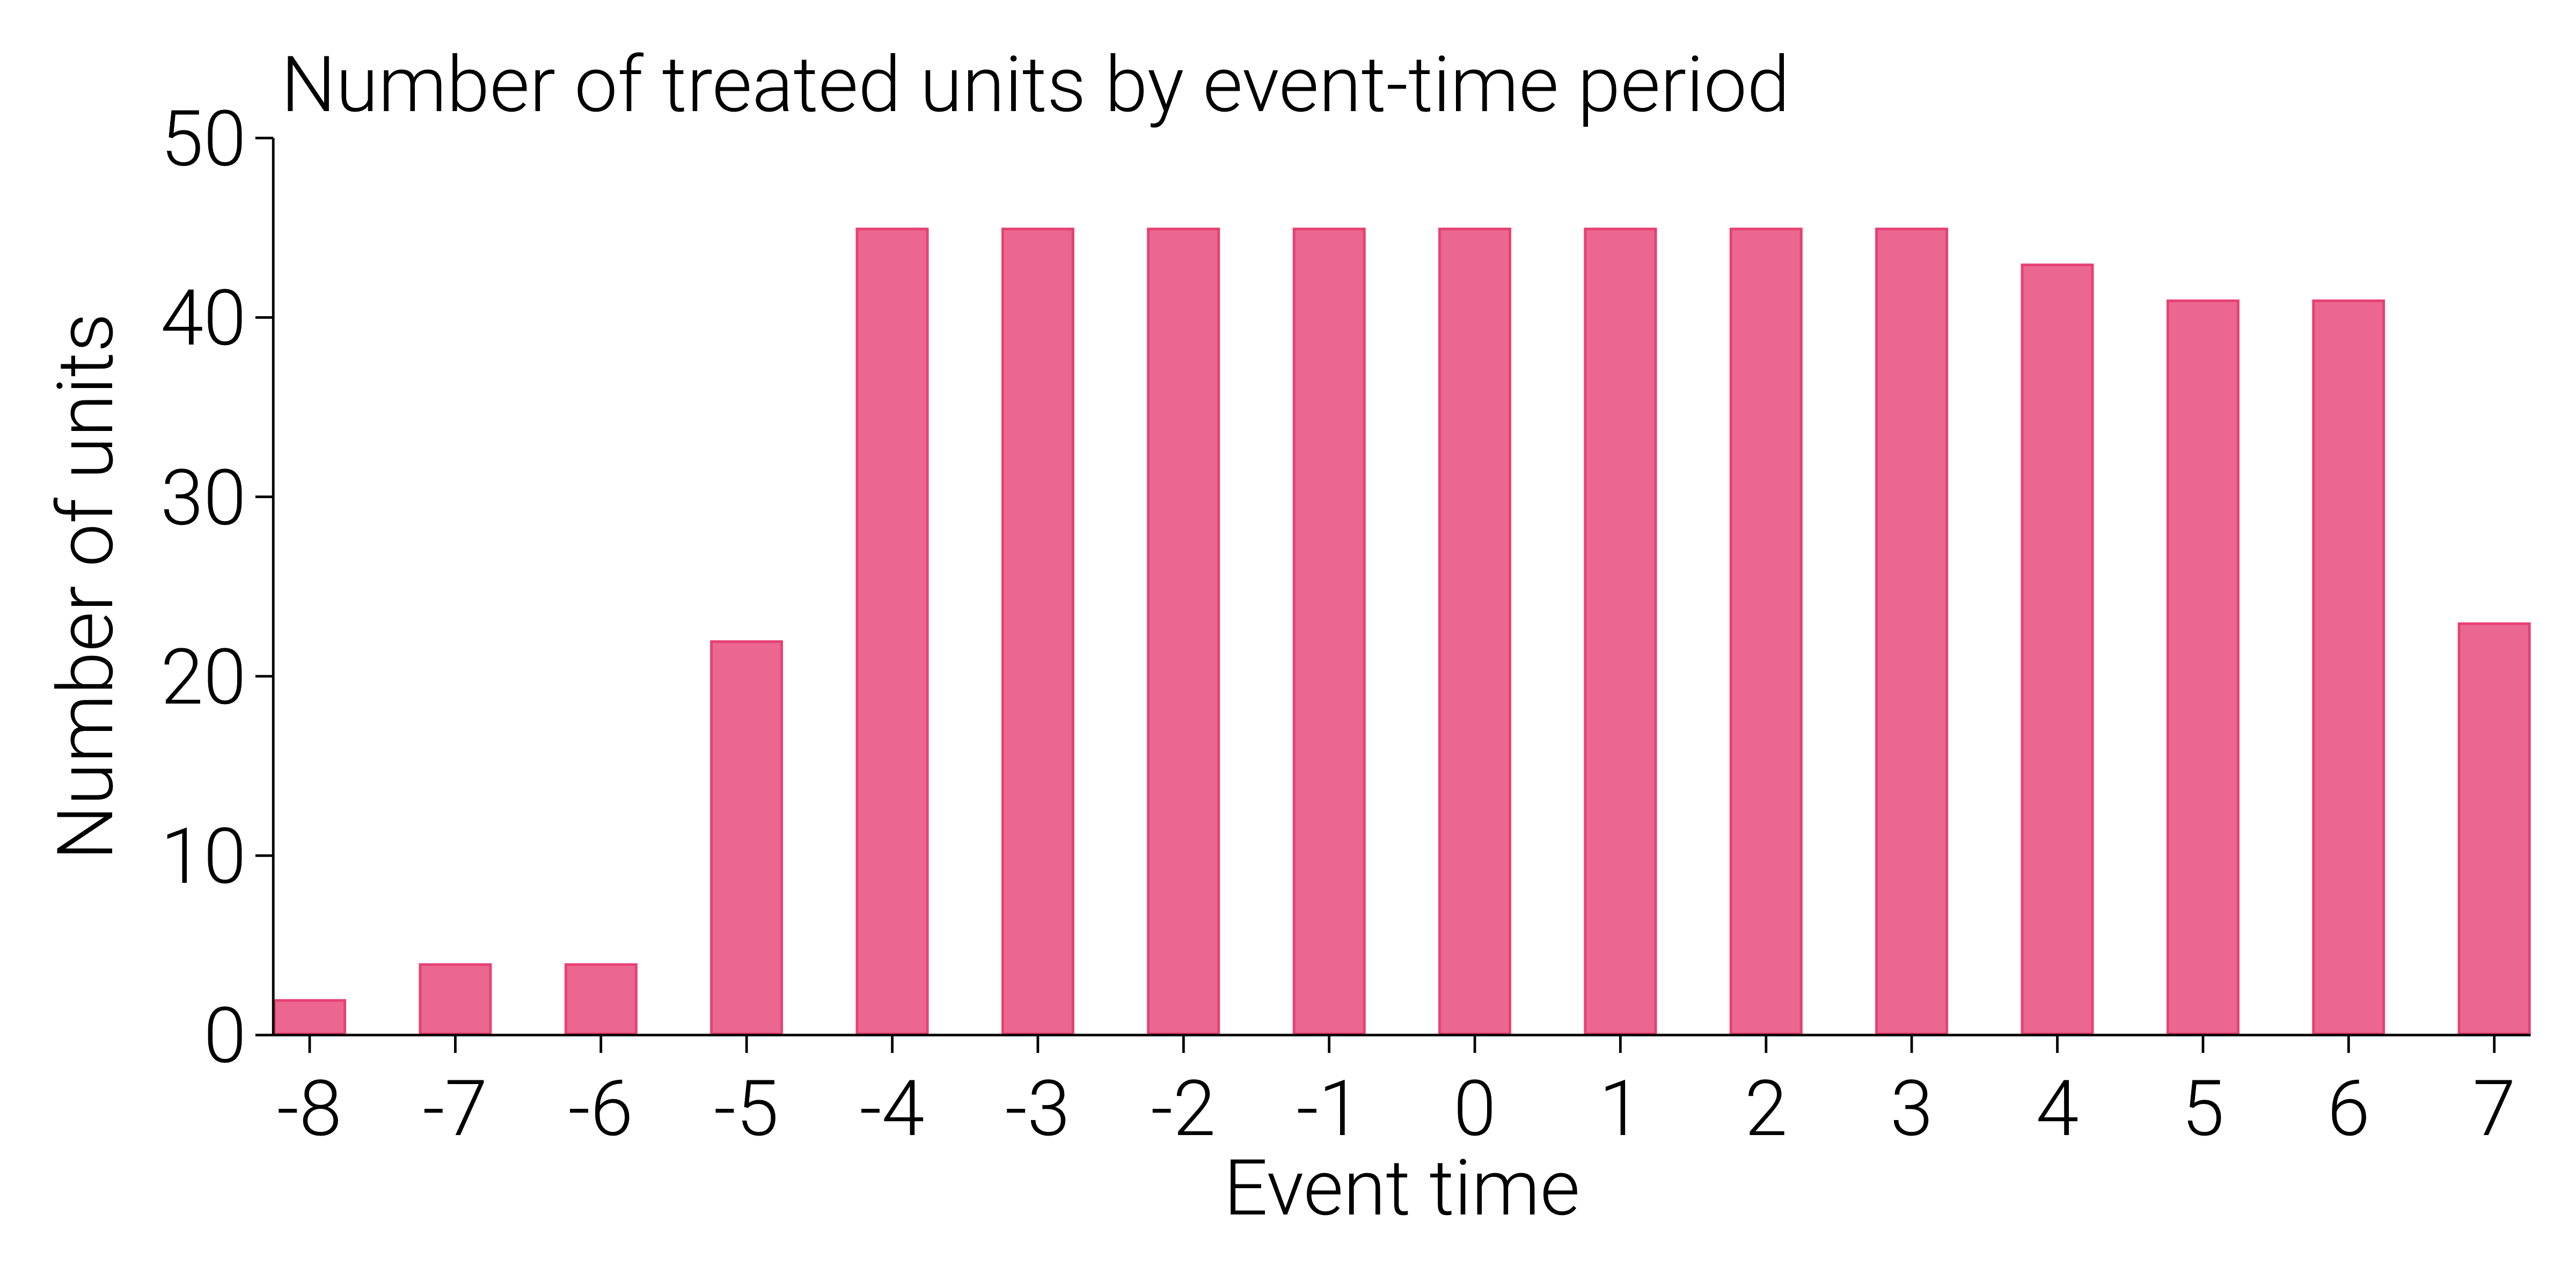
\includegraphics[width=1.0\linewidth]{../analysis/output/appendix/figure_a1_n_treated_units.png}
    \Fnote{
        This figure plots the number of treated states in each event-time period from $l = -8$ to $l = 7$, corresponding to the full set of indicators that are included in the event study specifications. 
        For clarity and due to the compositional changes in the set of treated states, the event studies do not display coefficients for periods from $l = -8$ to $l = -5$ and from $l = 5$ to $l = 7$.
	}
    \label{fig:treated-units-event-time}
\end{figure}


% Figure A2 - Event study - Placebo - MVA 
\newpage 
\begin{figure}[!ht]
    \caption[Event Study for Placebo (Motor Vehicle Accidents)]{Event Study for Placebo (Motor Vehicle Accidents)}
    \centering
    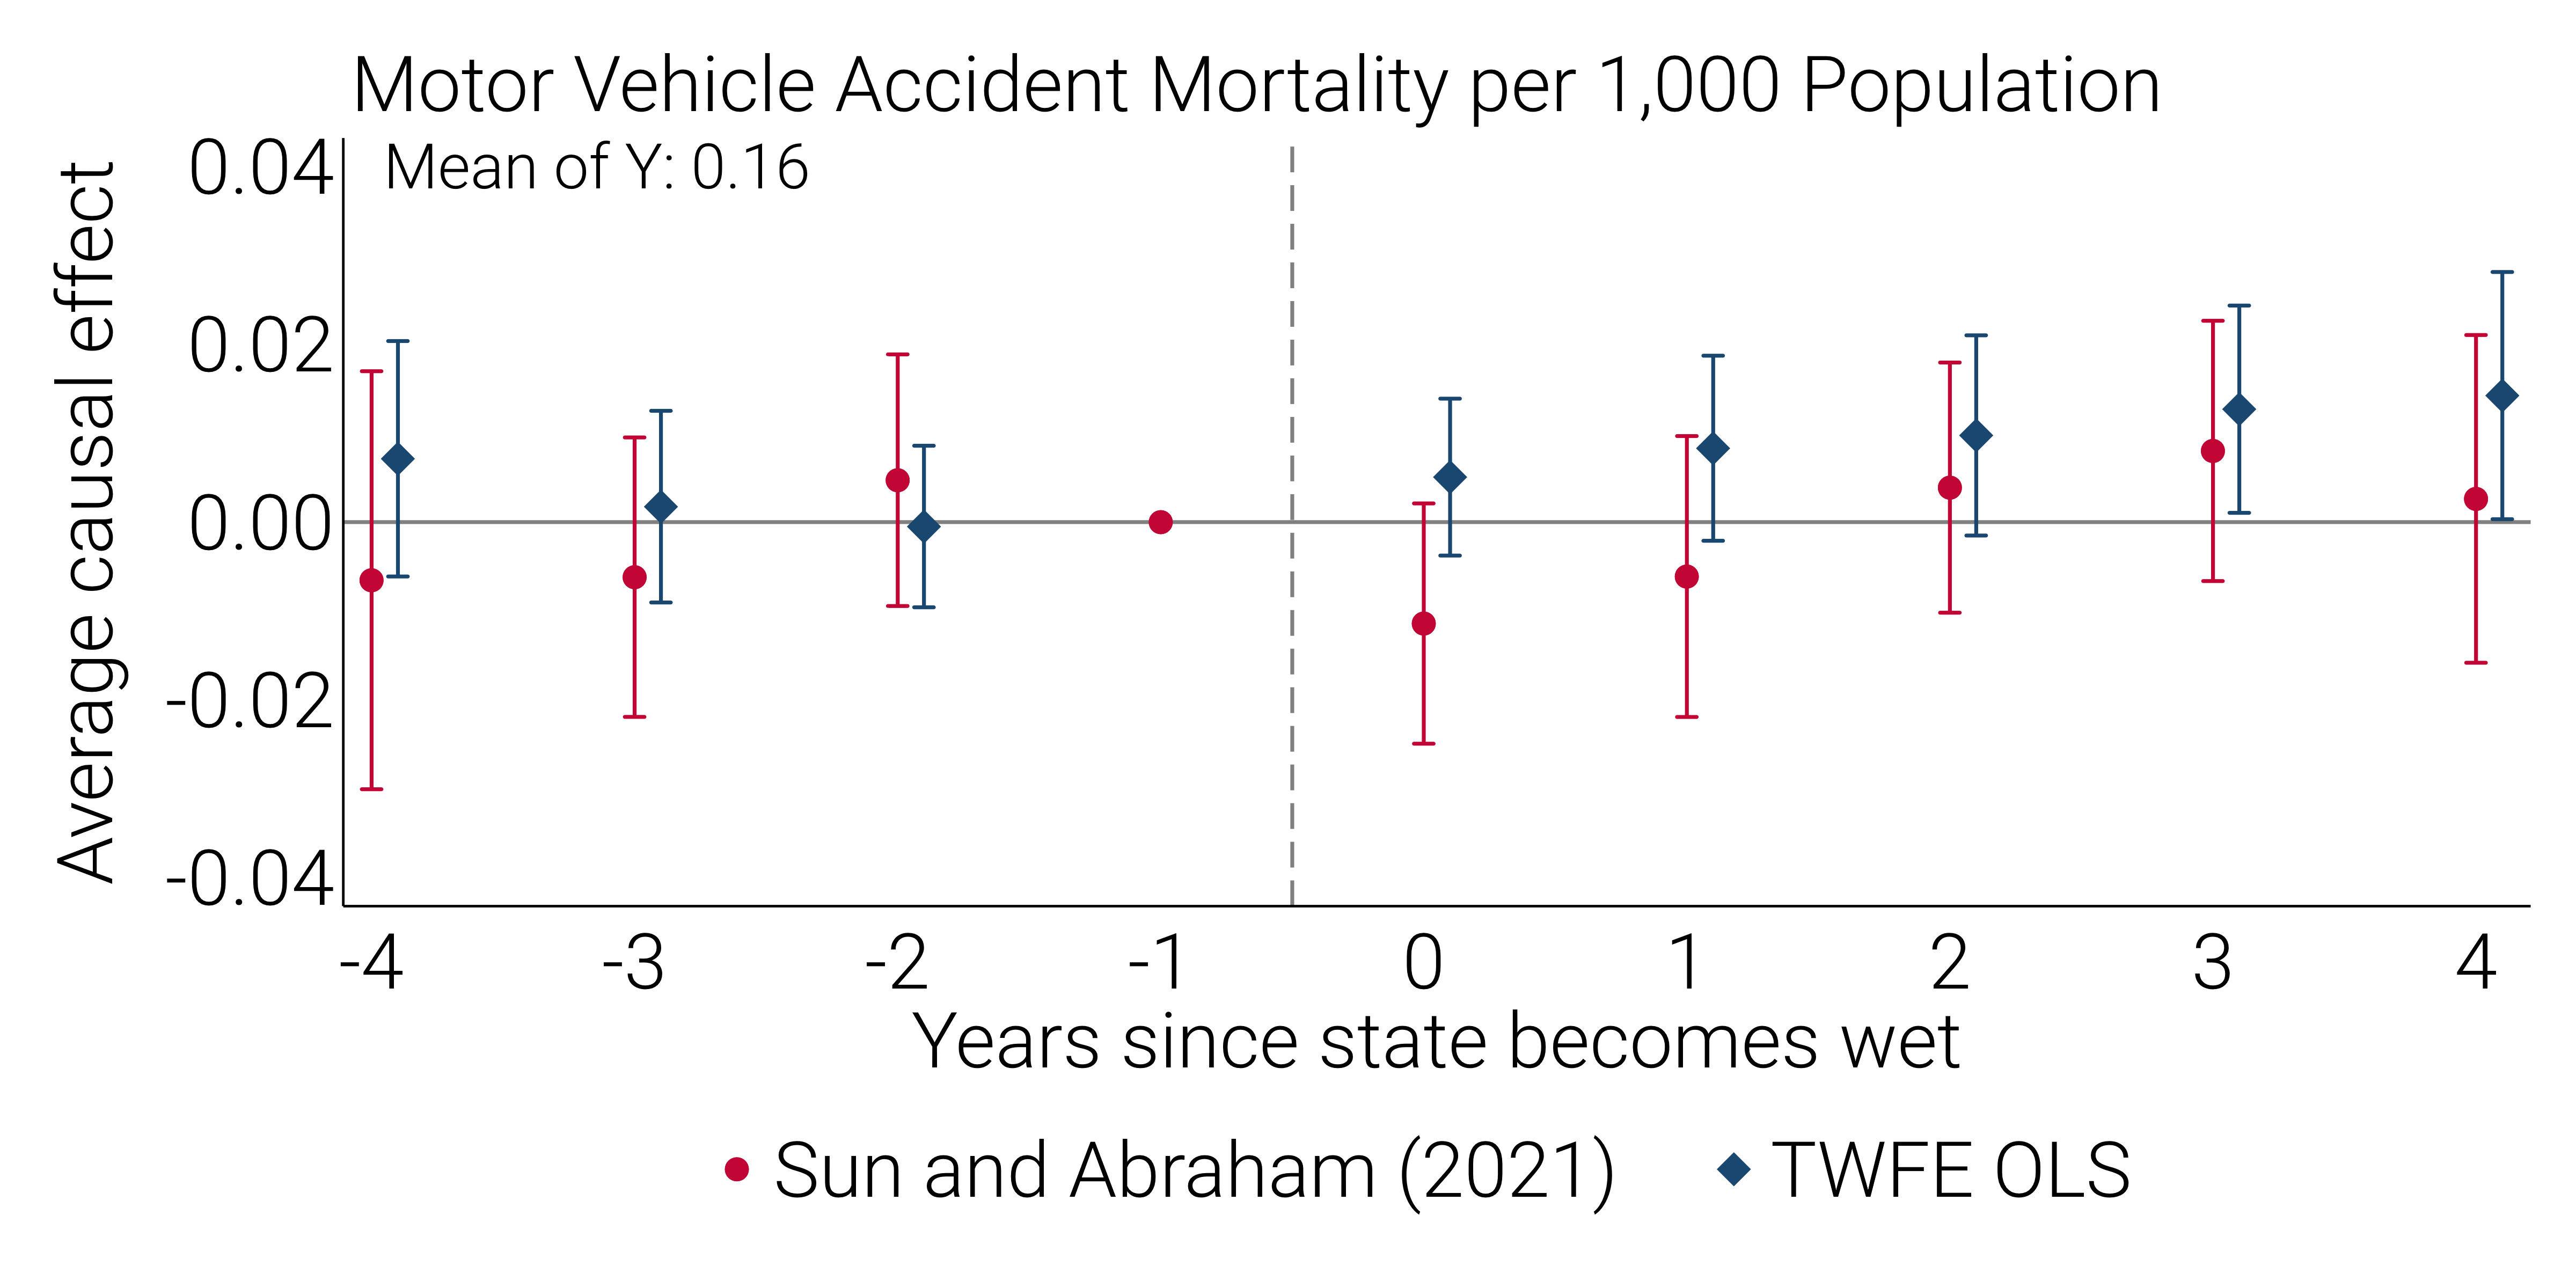
\includegraphics[width=1.0\linewidth]{../analysis/output/appendix/figure_a2_event_study_mv_acc.png}
    \Fnote{
        This figure displays an event study with motor vehicle accidents per 1,000 population as the dependent variable, using the same clustering, estimation techniques, observation weighting, sample, and specification as those in Figure~\ref{fig:event-study-cause-of-death}.  
        The sample includes the 1930 to 1941 birth cohorts. 
        The ``Mean of Y'' is the sample mean of the dependent variable for pre-treatment (1930-1933) birth cohorts in not-yet-treated states. 
        Mortality is observed between 1990 and 2004. 
        The coefficients for event-time periods $l = -8$ to $l = -5$ and $l = 5$ to $l = 7$ are omitted for clarity and due to the compositional changes in the set of treated states. 
        All specifications include birth year by year of death and state of birth by year of death fixed effects. 
        Observations are weighted by the surviving cohort size for each state of birth by year of birth by death year cell. 
        Standard errors are clustered at the state of birth by year of birth level. 
    }
    \label{fig:event-study-placebo-cause-of-death}
\end{figure}


% Figure A3 - Event study robustness - All-cause mortality, heart disease, stroke, and cancer
\newpage 
\newgeometry{top = 0.5in, bottom = 0.5in, right = 0.5in, left = 0.5in, footskip = 0.0in}
\begin{landscape}
\begin{figure}[!ht]
    \caption[Event Studies By Cause of Death)]{Event Studies By Cause of Death}
    \centering
    \begin{subfigure}{0.47\linewidth}
        \centering 
        \caption[All-Cause Mortality]{All-Cause Mortality}        
        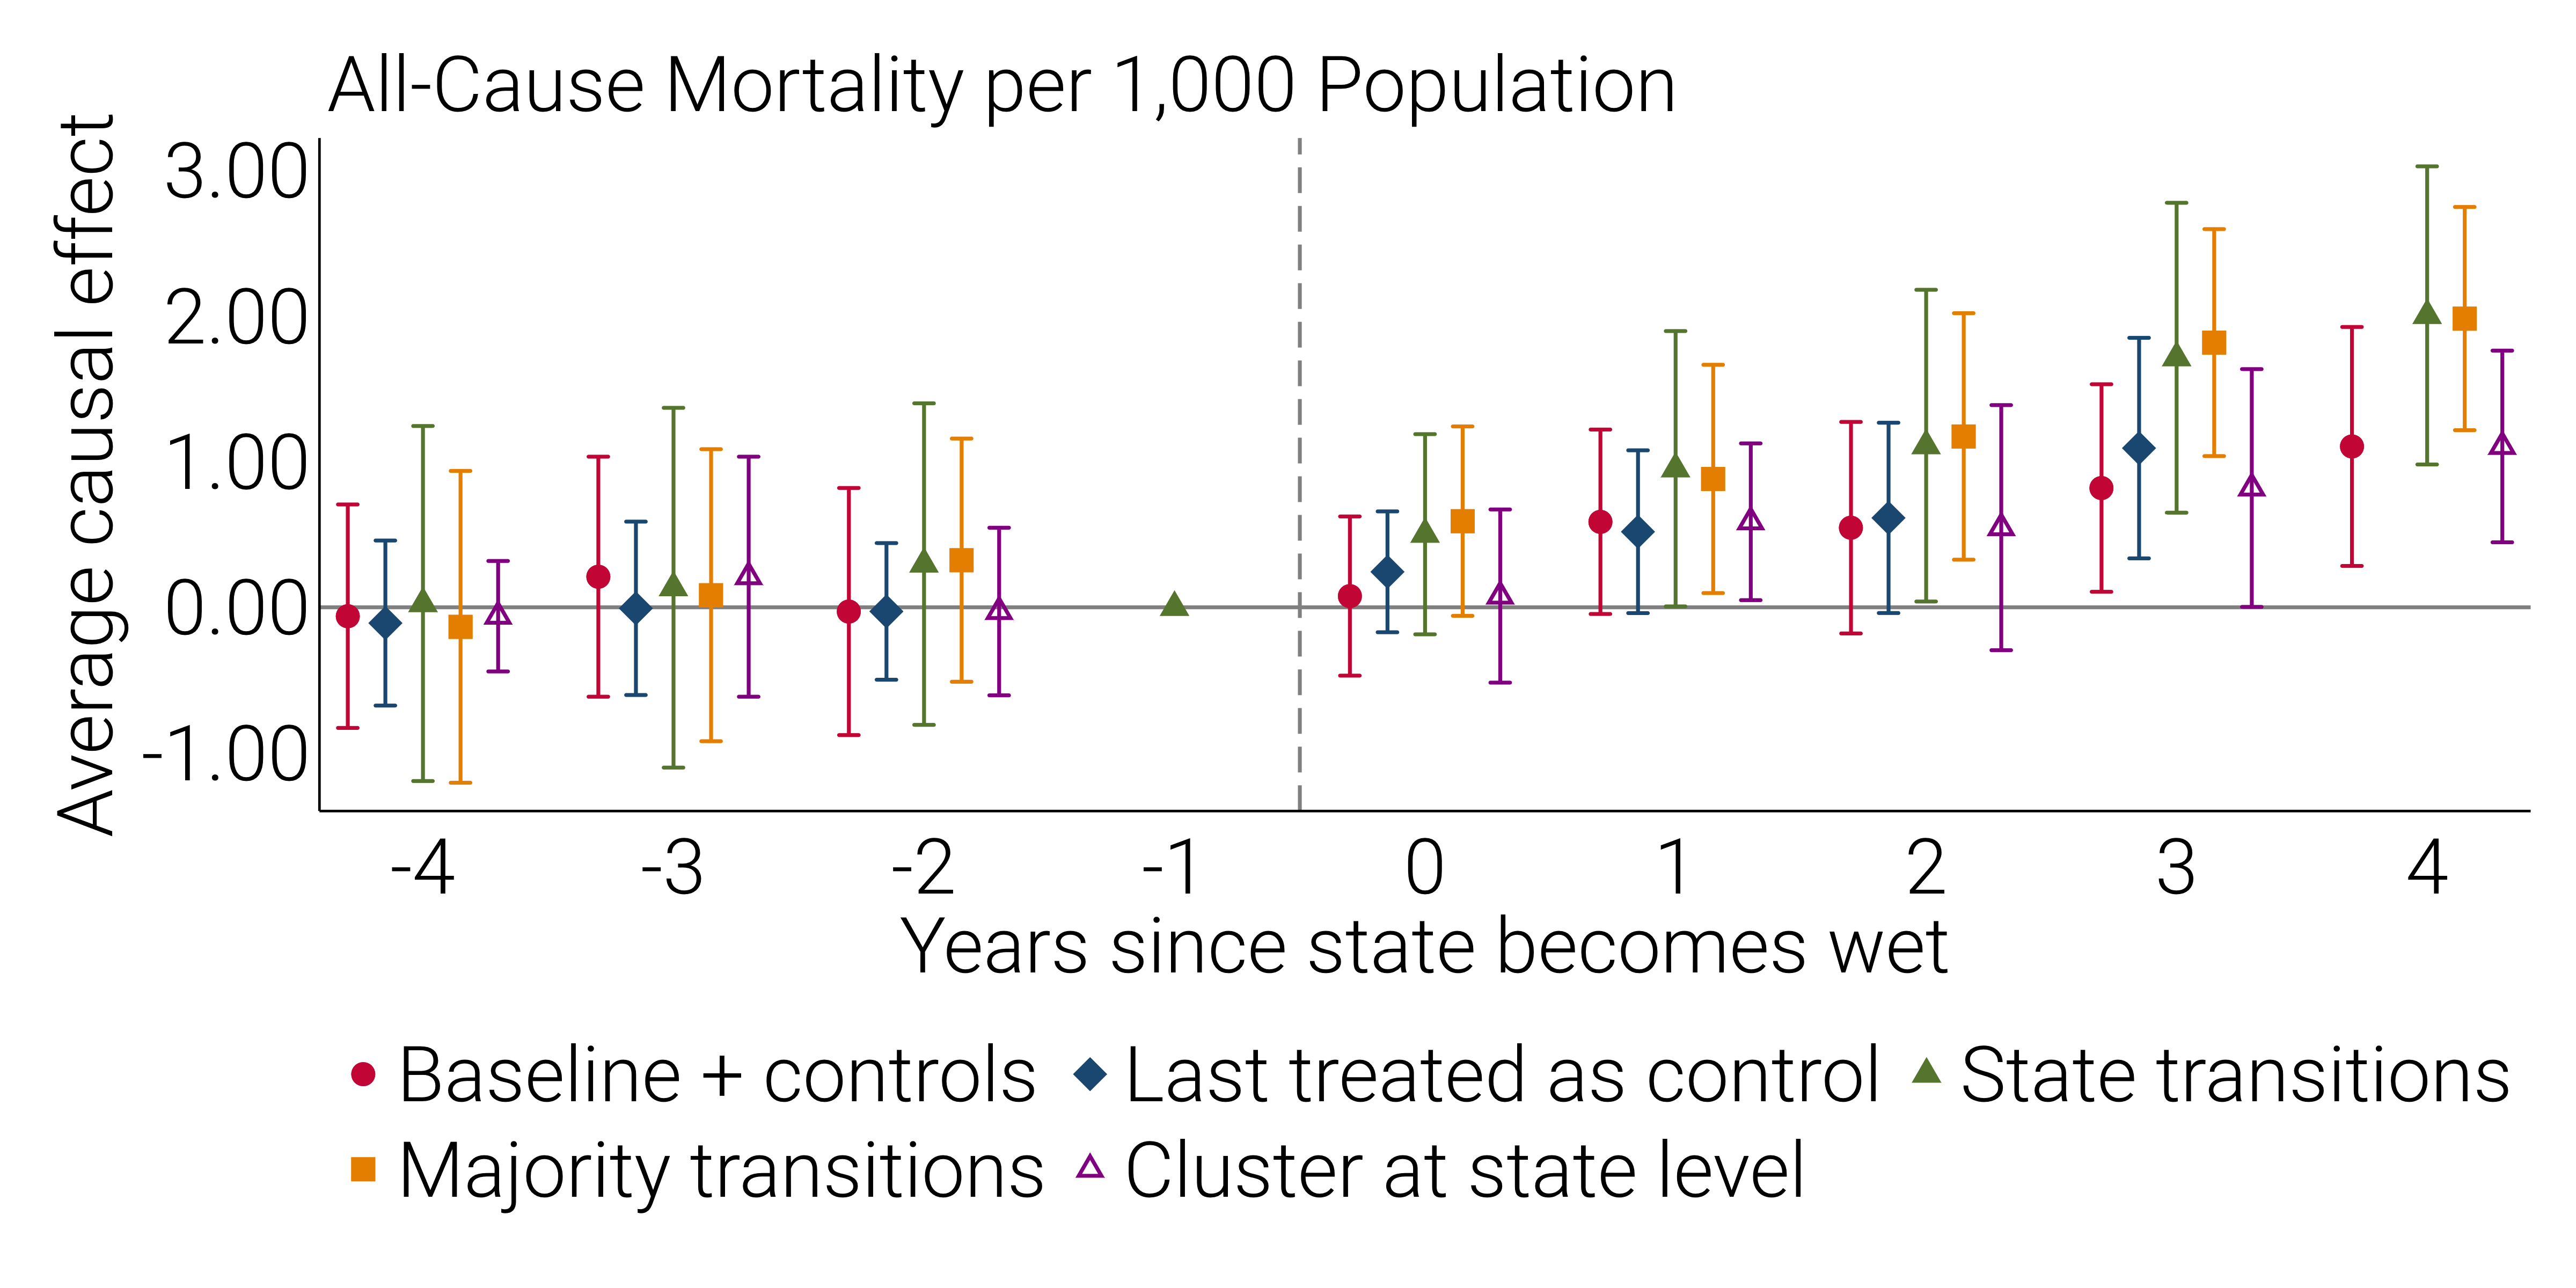
\includegraphics[width=1.0\linewidth]{../analysis/output/appendix/figure_a3a_es_robust_controls_deaths.png}
    \end{subfigure}
    \begin{subfigure}{0.47\linewidth}
        \centering 
        \caption[Heart Disease Mortality]{Heart Disease Mortality}        
        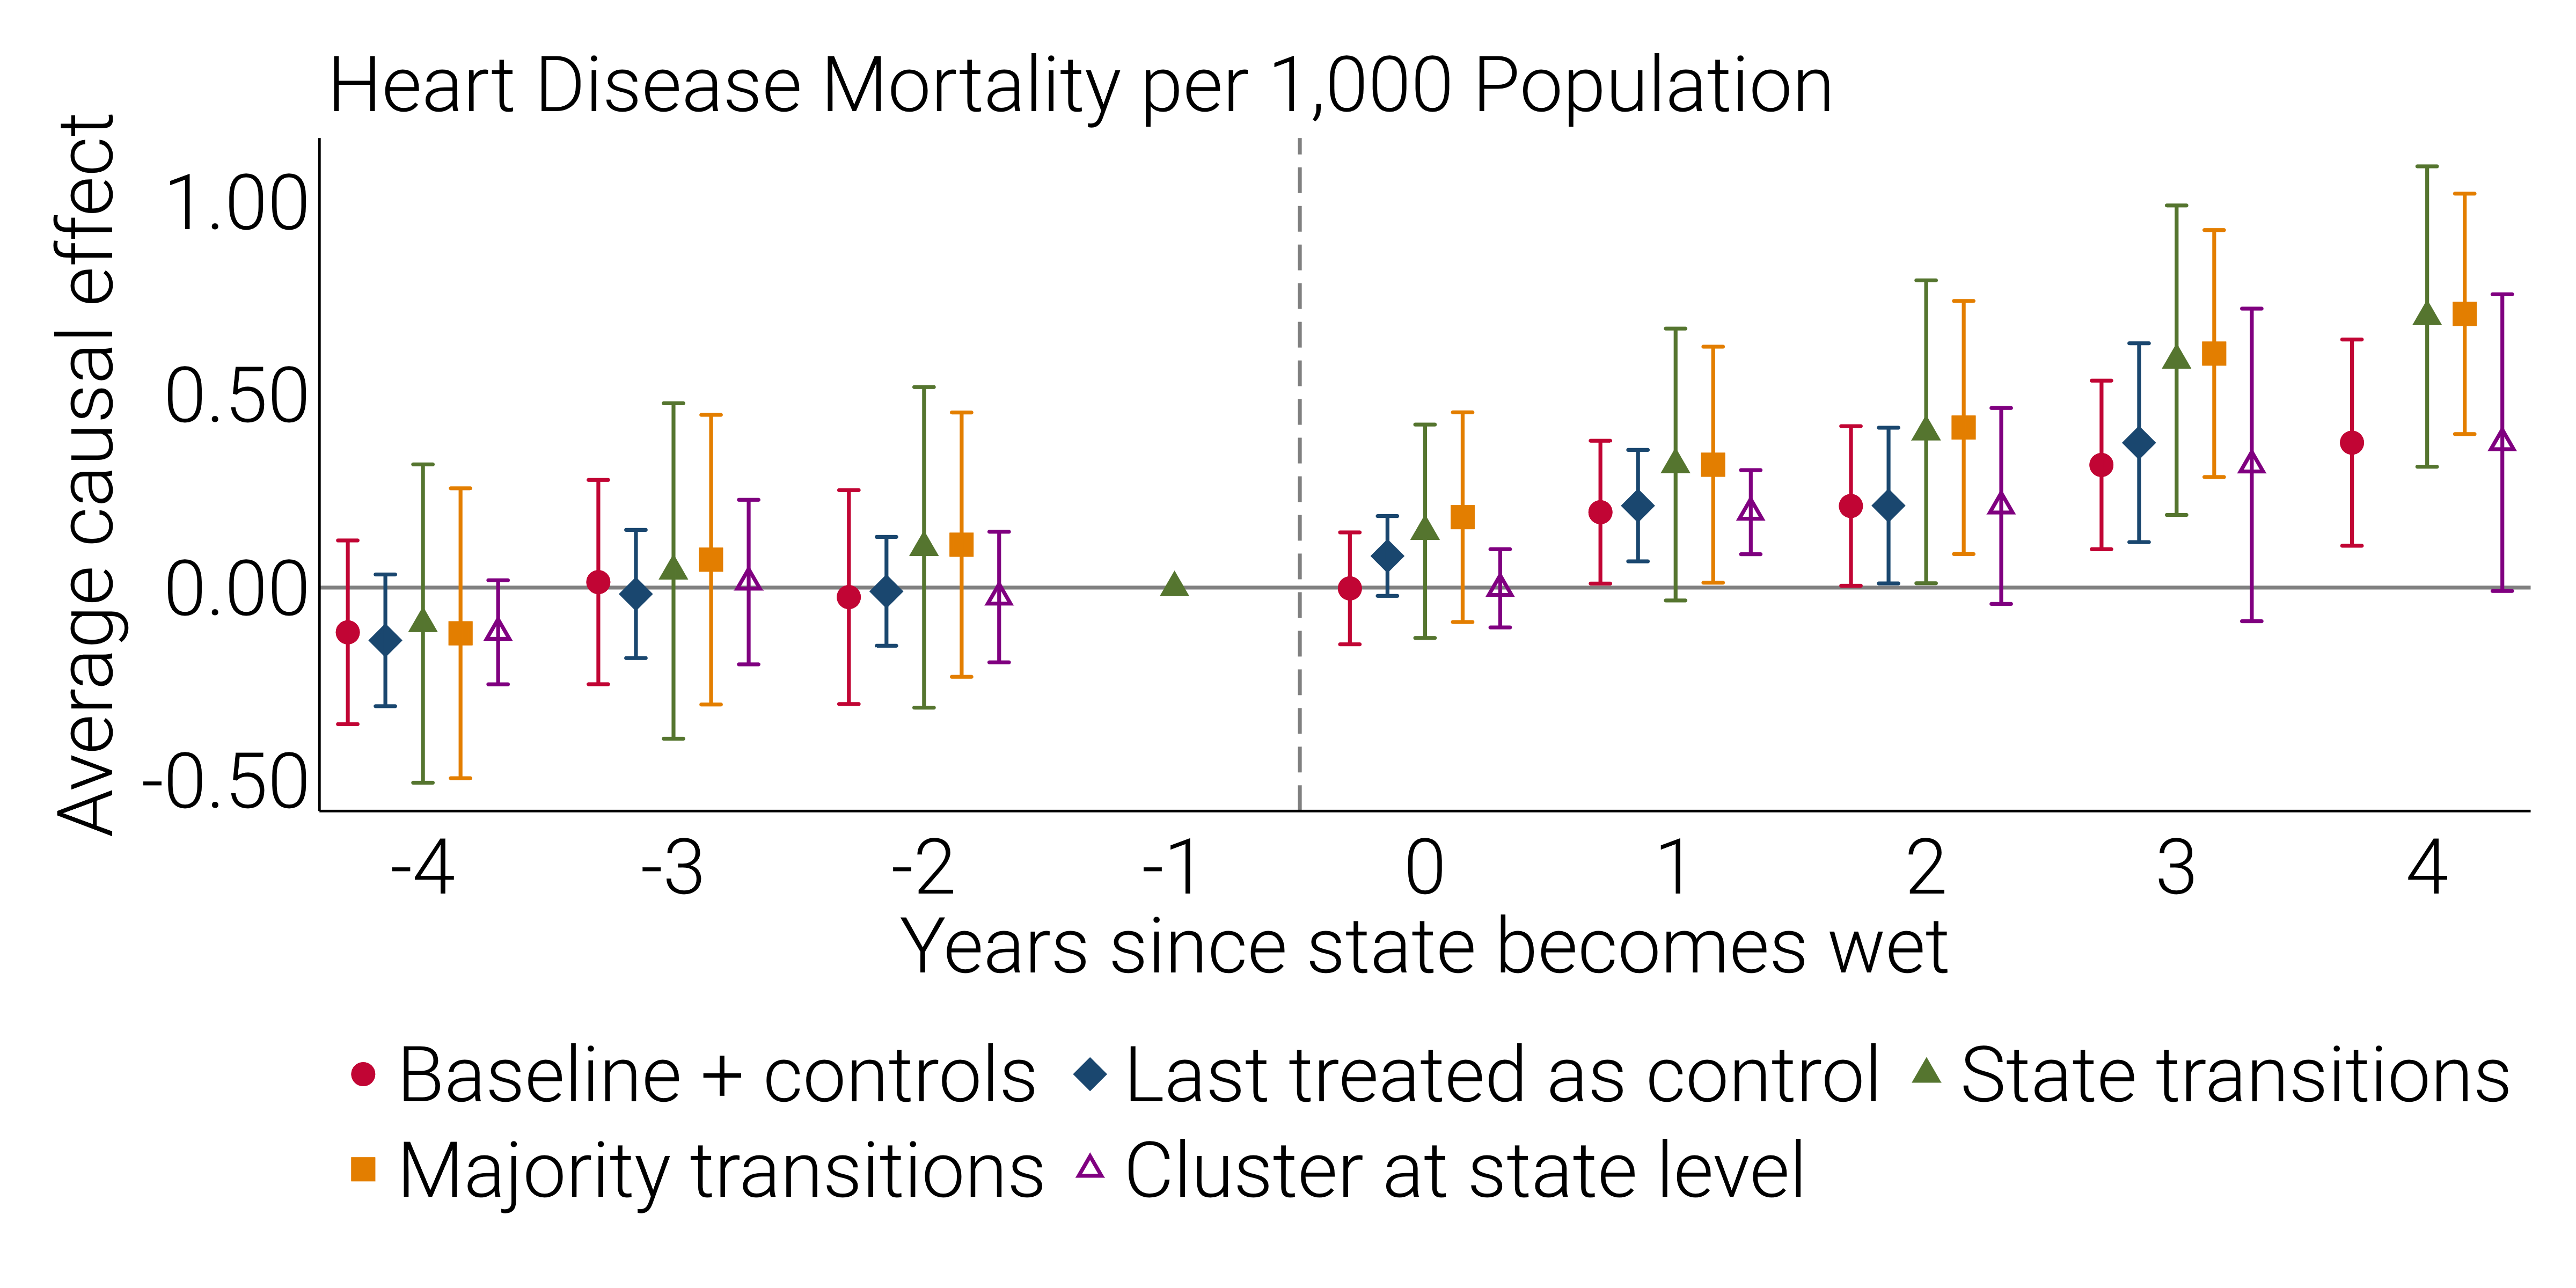
\includegraphics[width=1.0\linewidth]{../analysis/output/appendix/figure_a3b_es_robust_controls_heart.png}
    \end{subfigure}
    \begin{subfigure}{0.47\linewidth}
        \centering 
        \caption[Stroke Mortality]{Stroke Mortality}        
        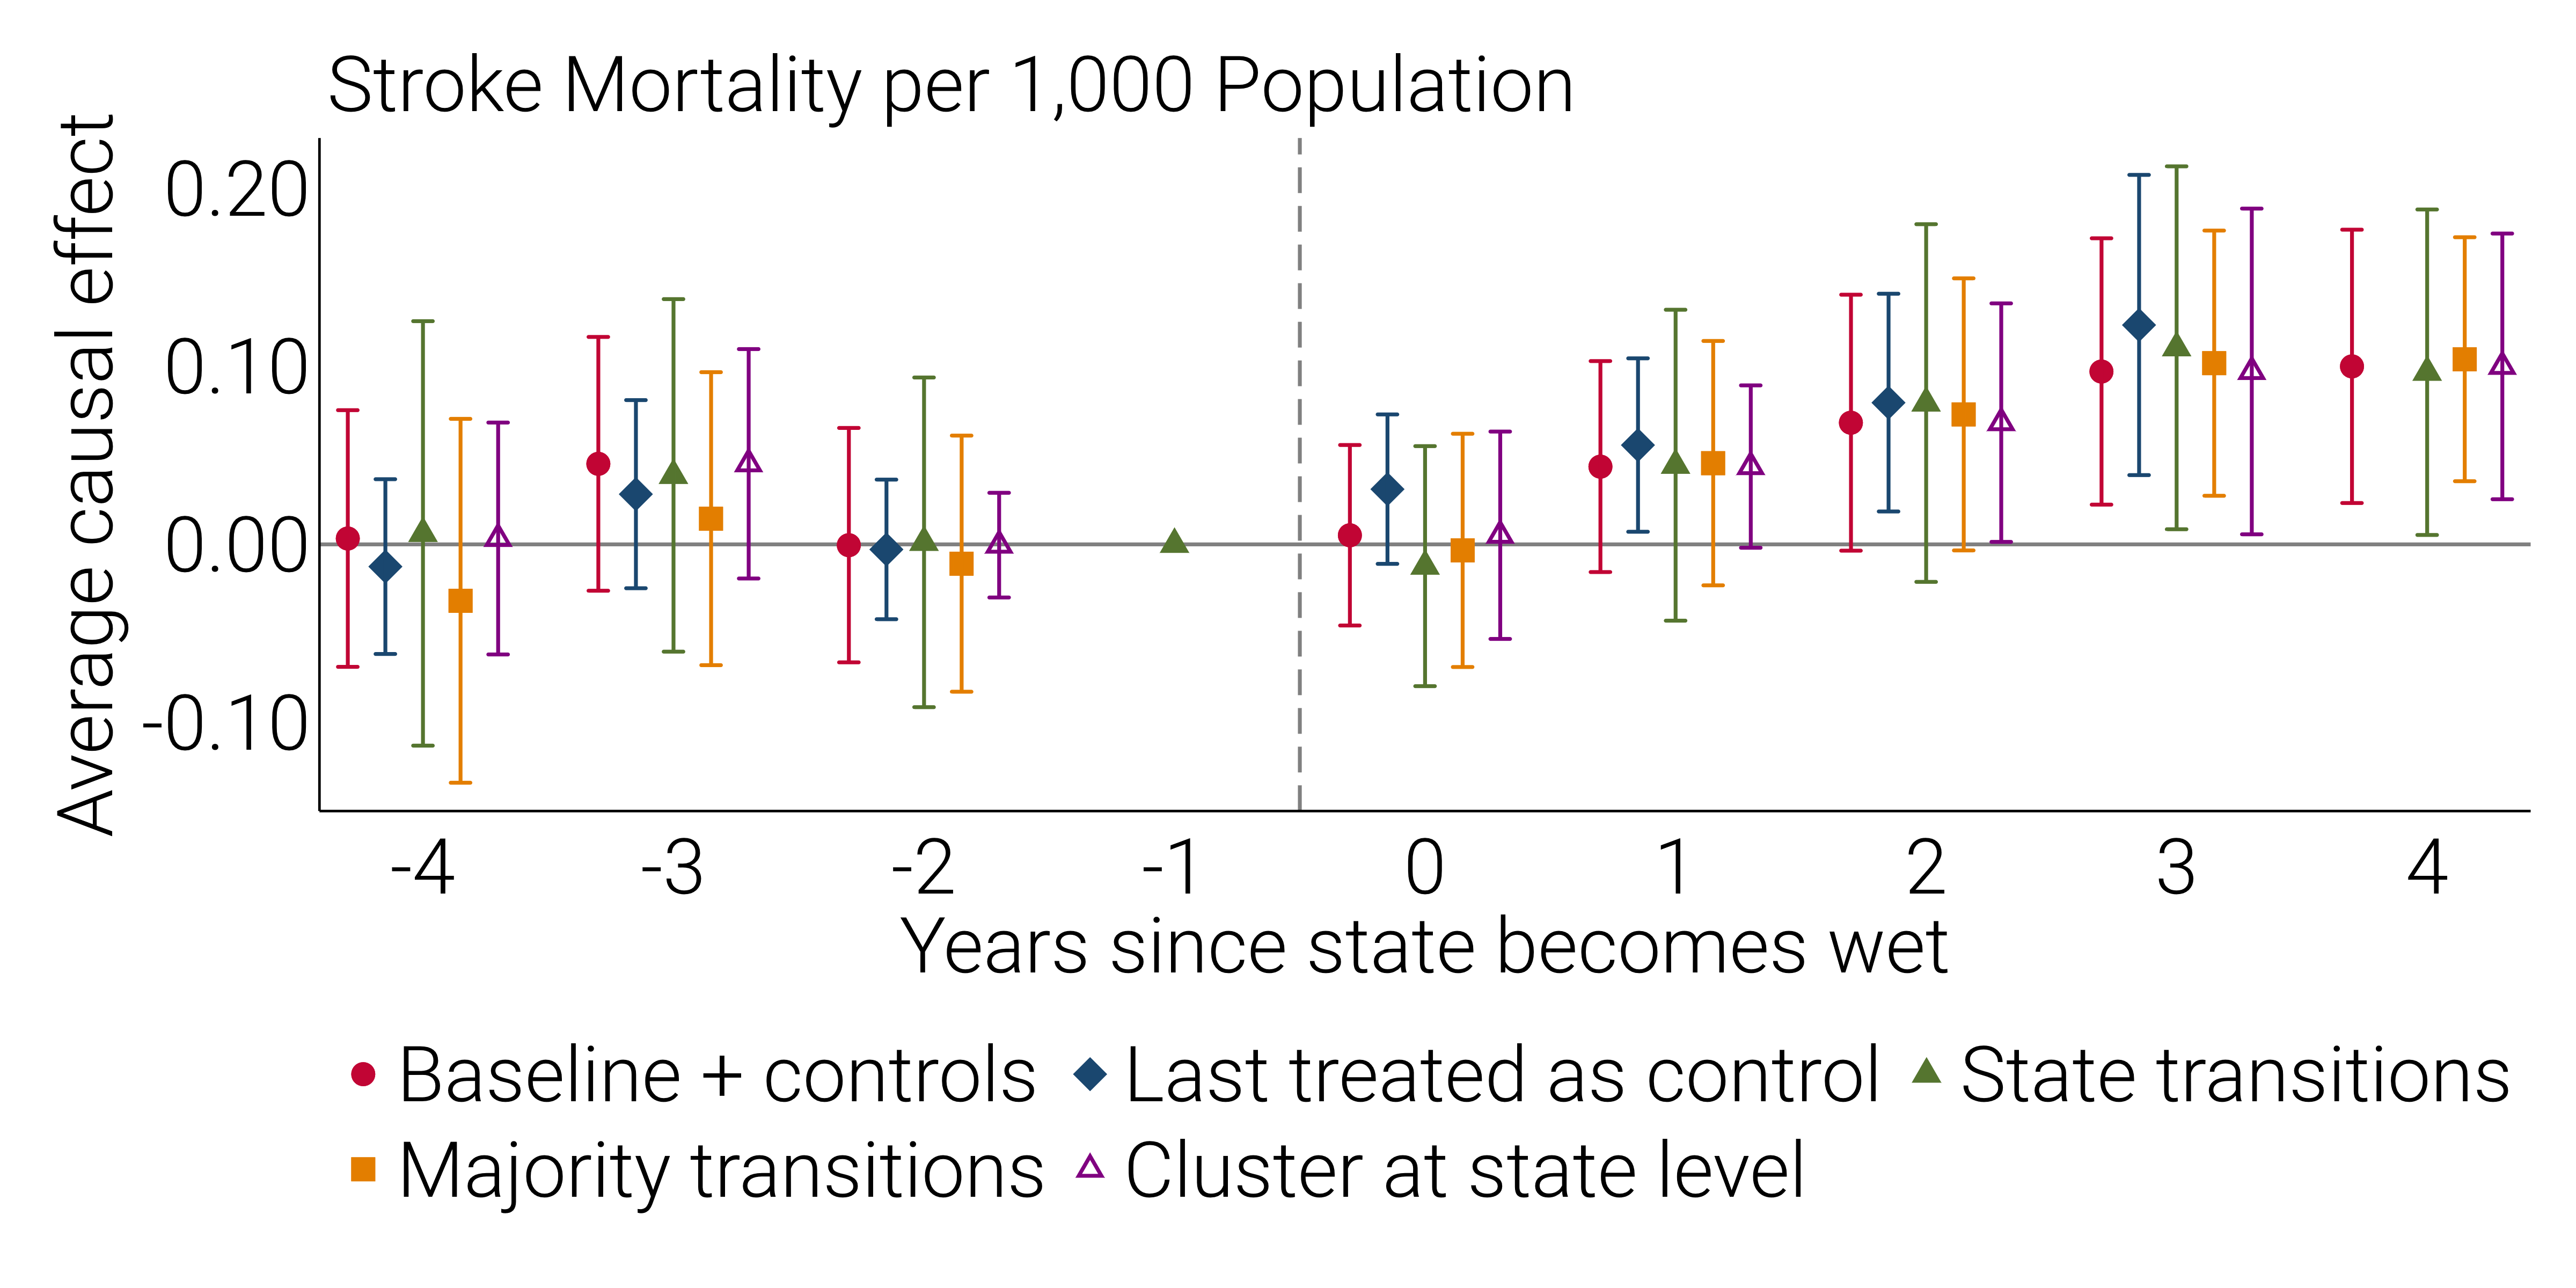
\includegraphics[width=1.0\linewidth]{../analysis/output/appendix/figure_a3c_es_robust_controls_stroke.png}
    \end{subfigure}    
    \begin{subfigure}{0.47\linewidth}
        \centering 
        \caption[Cancer Mortality]{Cancer Mortality}        
        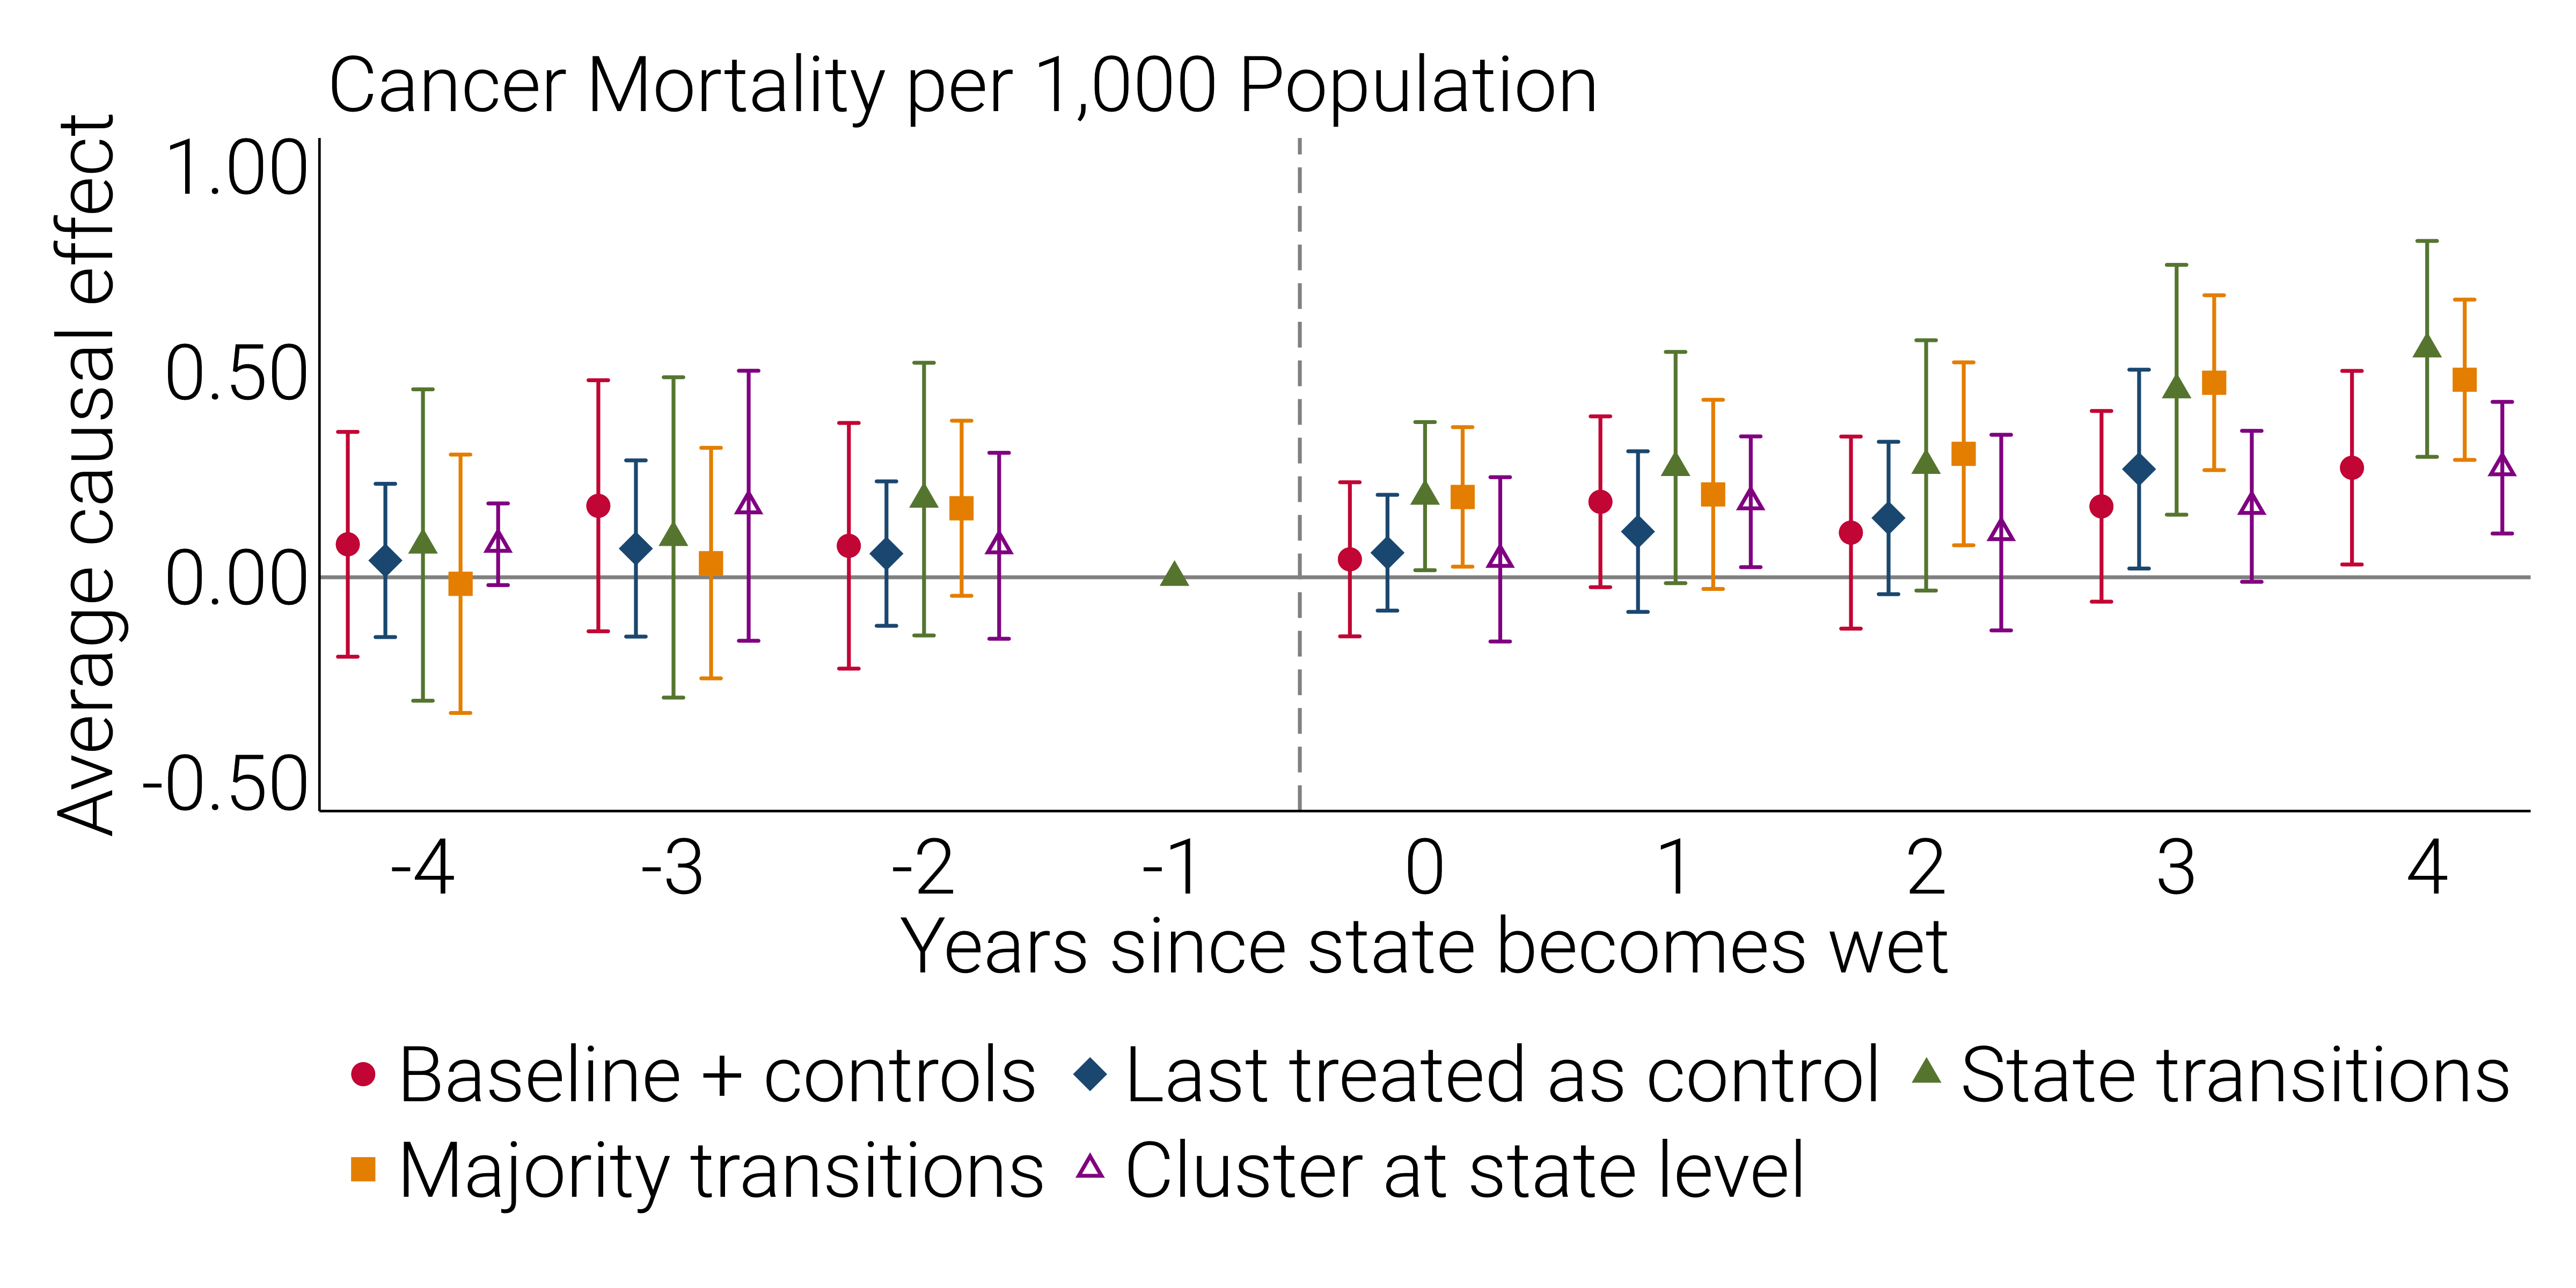
\includegraphics[width=1.0\linewidth]{../analysis/output/appendix/figure_a3d_es_robust_controls_cancer.png}
    \end{subfigure}
    \Fnote{
        The panels display event studies with all-cause mortality (panel A) or cause-specific mortality per 1,000 population as the dependent variable (heart disease in panel B, stroke in panel C, and cancer in panel D). 
        Each panel reports event studies using specifications corresponding to Figure~\ref{fig:event-study-cause-of-death} and sample restrictions corresponding to those applied in columns 2 to 6 of Table~\ref{tab:es-main-specs}. 
        All samples include the 1930 to 1941 birth cohorts. 
        The ``Mean of Y'' is the sample mean of the dependent variable for pre-treatment (1930-1933) birth cohorts in not-yet-treated states. 
        Mortality is observed between 1990 and 2004. 
        The coefficients for event-time periods $l = -8$ to $l = -5$ and $l = 5$ to $l = 7$ are omitted for clarity and due to the compositional changes in the set of treated states. 
        All specifications include birth year by year of death and state of birth by year of death fixed effects. 
        Observations are weighted by the surviving cohort size for each state of birth by year of birth by death year cell. 
        Standard errors are clustered at the state of birth by year of birth level except for the specification labeled ``Cluster at state level'' which is denoted by a triangle with a purple outline.
    }
    \label{fig:event-study-cause-of-death-robust-control}
\end{figure}
\end{landscape}
\restoregeometry


% Table A1: Crosswalk of ICD9 and ICD10 for Cause-Specific Mortality
\begin{table}[!ht]\centering
    \begin{adjustbox}{width=1.0\textwidth}
    \centering
    \begin{threeparttable}
        \caption{Crosswalk of ICD9 and ICD10 for Cause-Specific Mortality \label{tab:icd-crosswalk}}
        \vspace{.25ex}
        \textsymbols
        \begin{tabular}{lll}
        \toprule
        \estinput{../analysis/output/appendix/table_a1_icd_crosswalk.tex}
        \bottomrule
        \addlinespace[.75ex]
        \end{tabular}
        \Fignote{ICD9 was used until 1998 while ICD10 has been used since in the Multiple Cause of Death data. Source: \citeApp{national_center_for_health_statistics_us_comparability_2001}.}
    \end{threeparttable}
    \end{adjustbox}
\end{table}


% Table A2. Bounding selection into survival. By Year. Main Sample.
\newpage
\begin{table}[!ht]\centering
    \begin{adjustbox}{width=1.0\textwidth}
    \centering
      \begin{threeparttable}
       \caption{Bounding the Magnitude of Selection due to Repeal-Induced Infant Mortality: Effects on Mortality by Year of Death, 1990-2004.}
       \estauto{../analysis/output/appendix/table_a2_bounding_infant_deaths_by_year_1990_start.tex}{6}{S[table-format=2.3,table-column-width=20mm, table-alignment = center]}
        \label{tab:bounding-selection-into-survival-by-year-1990-start} 
        \Fignote{
            The unit of observation is the annual mortality rate for a given state of birth by year of birth cohort. 
            The sample includes the 1930 to 1941 birth cohorts. 
            The ``Mean of Y'' is the sample mean of the dependent variable for pre-treatment (1930-1933) birth cohorts in not-yet-treated states. 
            Mortality is observed between 1990 and 2004. 
            Each coefficient is the average of the \citeApp{sun_estimating_2021} event study coefficients from $l = 0$ to $l = 4$ and represents the average change in the later-life all-cause mortality rate attributable to in utero exposure to the first five years of federal prohibition’s repeal. 
            In all columns, observations are treated (i.e., the indicator for wet status equals one) if at least some alcohol sales were allowed anywhere within the state of birth in the year of birth. 
            Column 1 corresponds to our main estimates reported in Column 2 of Table~\ref{tab:es-main-specs}. 
            All columns include state of birth by death year and year of birth by death year fixed effects, as well as control variables for the log of per capita New Deal spending and the log of per capita real disposable personal income at the state level. 
            In Columns 1 to 3, the dependent variable is the number of deaths per 1,000 population. 
            Columns 2 to 5 drop South Dakota and Texas due to missing infant mortality data. 
            In Columns 1 and 2, observations are weighted by the surviving cohort size for each state of birth by year of birth by death year cell. 
            Columns 3 to 5 adjust the dependent variable and the weights in the main specification by the number of infant deaths attributable to the repeal of Federal Prohibition. 
            \citeApp{jacks_infant_2021} find that repeal is associated with a 4.0\% increase in infant mortality rates in wet counties. 
            Thus, if we let $d_{st}$ denote the number of infant deaths in state $s$ in year $t$, then the number of infant deaths attributable to the repeal of Federal Prohibition is $d^*_{st} = d_{st} - d_{st}/1.04$. 
            We refer to $d^*_{st}$ as ``treated'' infant deaths. 
            Columns 3 to 5 add treated infant deaths to the surviving cohort size for each state of birth by year of birth by death year cell and uses this expanded cohort size to weight observations.
            Columns 4 and 5 additionally use this expanded cohort size to adjust the surviving cohort size in the denominator of the dependent variable.
            Column 5 adds treated infant deaths to the count of later-life deaths in the numerator of the dependent variable. 
            Standard errors are clustered at the state of birth by year of birth level. 
            Standard errors are in parentheses; t-statistics reported below standard errors in brackets.
          }
      \end{threeparttable}
     \end{adjustbox}
\end{table}

% Table A3. Effects on Mortality between 1940 and 1990.
\begin{landscape}
    \begin{table}[!ht]\centering
        \begin{adjustbox}{width=1.0\textwidth}
        \centering
          \begin{threeparttable}
           \caption{Effects on Mortality between 1940 and 1990.}
           \estauto{../analysis/output/appendix/table_a3_life_cycle_mortality.tex}{8}{S[table-format=2.3,table-column-width=20mm, table-alignment = center]}
            \label{tab:life-cycle-mortality-abst} 
            \Fignote{
                The unit of observation is the annual mortality rate for a given state of birth by year of birth cohort. 
                The sample includes the 1930 to 1941 birth cohorts. 
                The ``Mean of Y'' is the sample mean of the dependent variable for pre-treatment (1930-1933) birth cohorts in not-yet-treated states. 
                Mortality is observed between 1990 and 2004. 
                Each coefficient is the average of the \citeApp{sun_estimating_2021} event study coefficients from $l = 0$ to $l = 4$ and represents the average change in the later-life all-cause mortality rate attributable to in utero exposure to the first five years of federal prohibition’s repeal. 
                In all columns, observations are treated (i.e., the indicator for wet status equals one) if at least some alcohol sales were allowed anywhere within the state of birth in the year of birth. 
                Column 1 corresponds to our preferred estimate when using cumulative mortality as the outcome, which is reported in Column 2 of Table~\ref{tab:did-cumulative-mortality}. 
                All columns include state of birth and year of birth fixed effects, as well as control variables for the log of per capita New Deal spending and the log of per capita real disposable personal income at the state level. 
                Observations are weighted by the surviving cohort size in 1990 for each state of birth by year of birth cell. 
                In Columns 1 to 3, the dependent variable is cumulative all-cause deaths between 1990 and 2004 per 1,000 population in 1990. 
                Columns 2, 4, and 6 drop Washington state due to missing data in the preliminary release of the 1950 full-count census from IPUMS \citepApp{ruggles_ipums_2023}. 
                Columns 3, 5, and 7 drop the 1940 and 1941 birth cohorts because these cohorts are not observed in their entirety in the 1940 full-count census.
                Our results for cumulative mortality are unaffected by these sample restrictions. 
                In the remaining columns, the dependent variable is the mortality rate proxies by the change in surviving cohort size between a baseline census (1940 or 1950) and the start of our sample window (1979 or 1990) per 1,000 surviving individuals in the baseline population.
                We consider the following intervals: 1950-1990 (column 4), 1940-1990 (column 5), 1950-1979 (column 6), and 1940-1979 (column 7).
                Standard errors are clustered at the state of birth by year of birth level. 
                Standard errors are in parentheses; t-statistics reported below standard errors in brackets.
              }
          \end{threeparttable}
         \end{adjustbox}
    \end{table}
\end{landscape}

%----------------------------------------------------%
%       Appendix B: Extended Panel
%----------------------------------------------------%

\FloatBarrier
% Figure B1 - Event study - Mortality from 1979 to 2004 - All-cause mortality, heart disease, cancer, and stroke
\newpage 
\newgeometry{top = 0.5in, bottom = 0.5in, right = 0.5in, left = 0.5in, footskip = 0.0in}
\begin{landscape}
\section[Results from Extended Panel, 1979-2004]{Results from Extended Panel, 1979-2004\label{sec:app-extend-panel}}
\setcounter{figure}{0}\renewcommand{\thefigure}{\ref{sec:app-extend-panel}\arabic{figure}}
\begin{figure}[!ht]
    \caption[Event Studies, 1979-2004]{Event Studies, 1979-2004}
    \centering
    \begin{subfigure}{0.49\linewidth}
        \centering 
        \caption[All-Cause Mortality]{All-Cause Mortality}        
        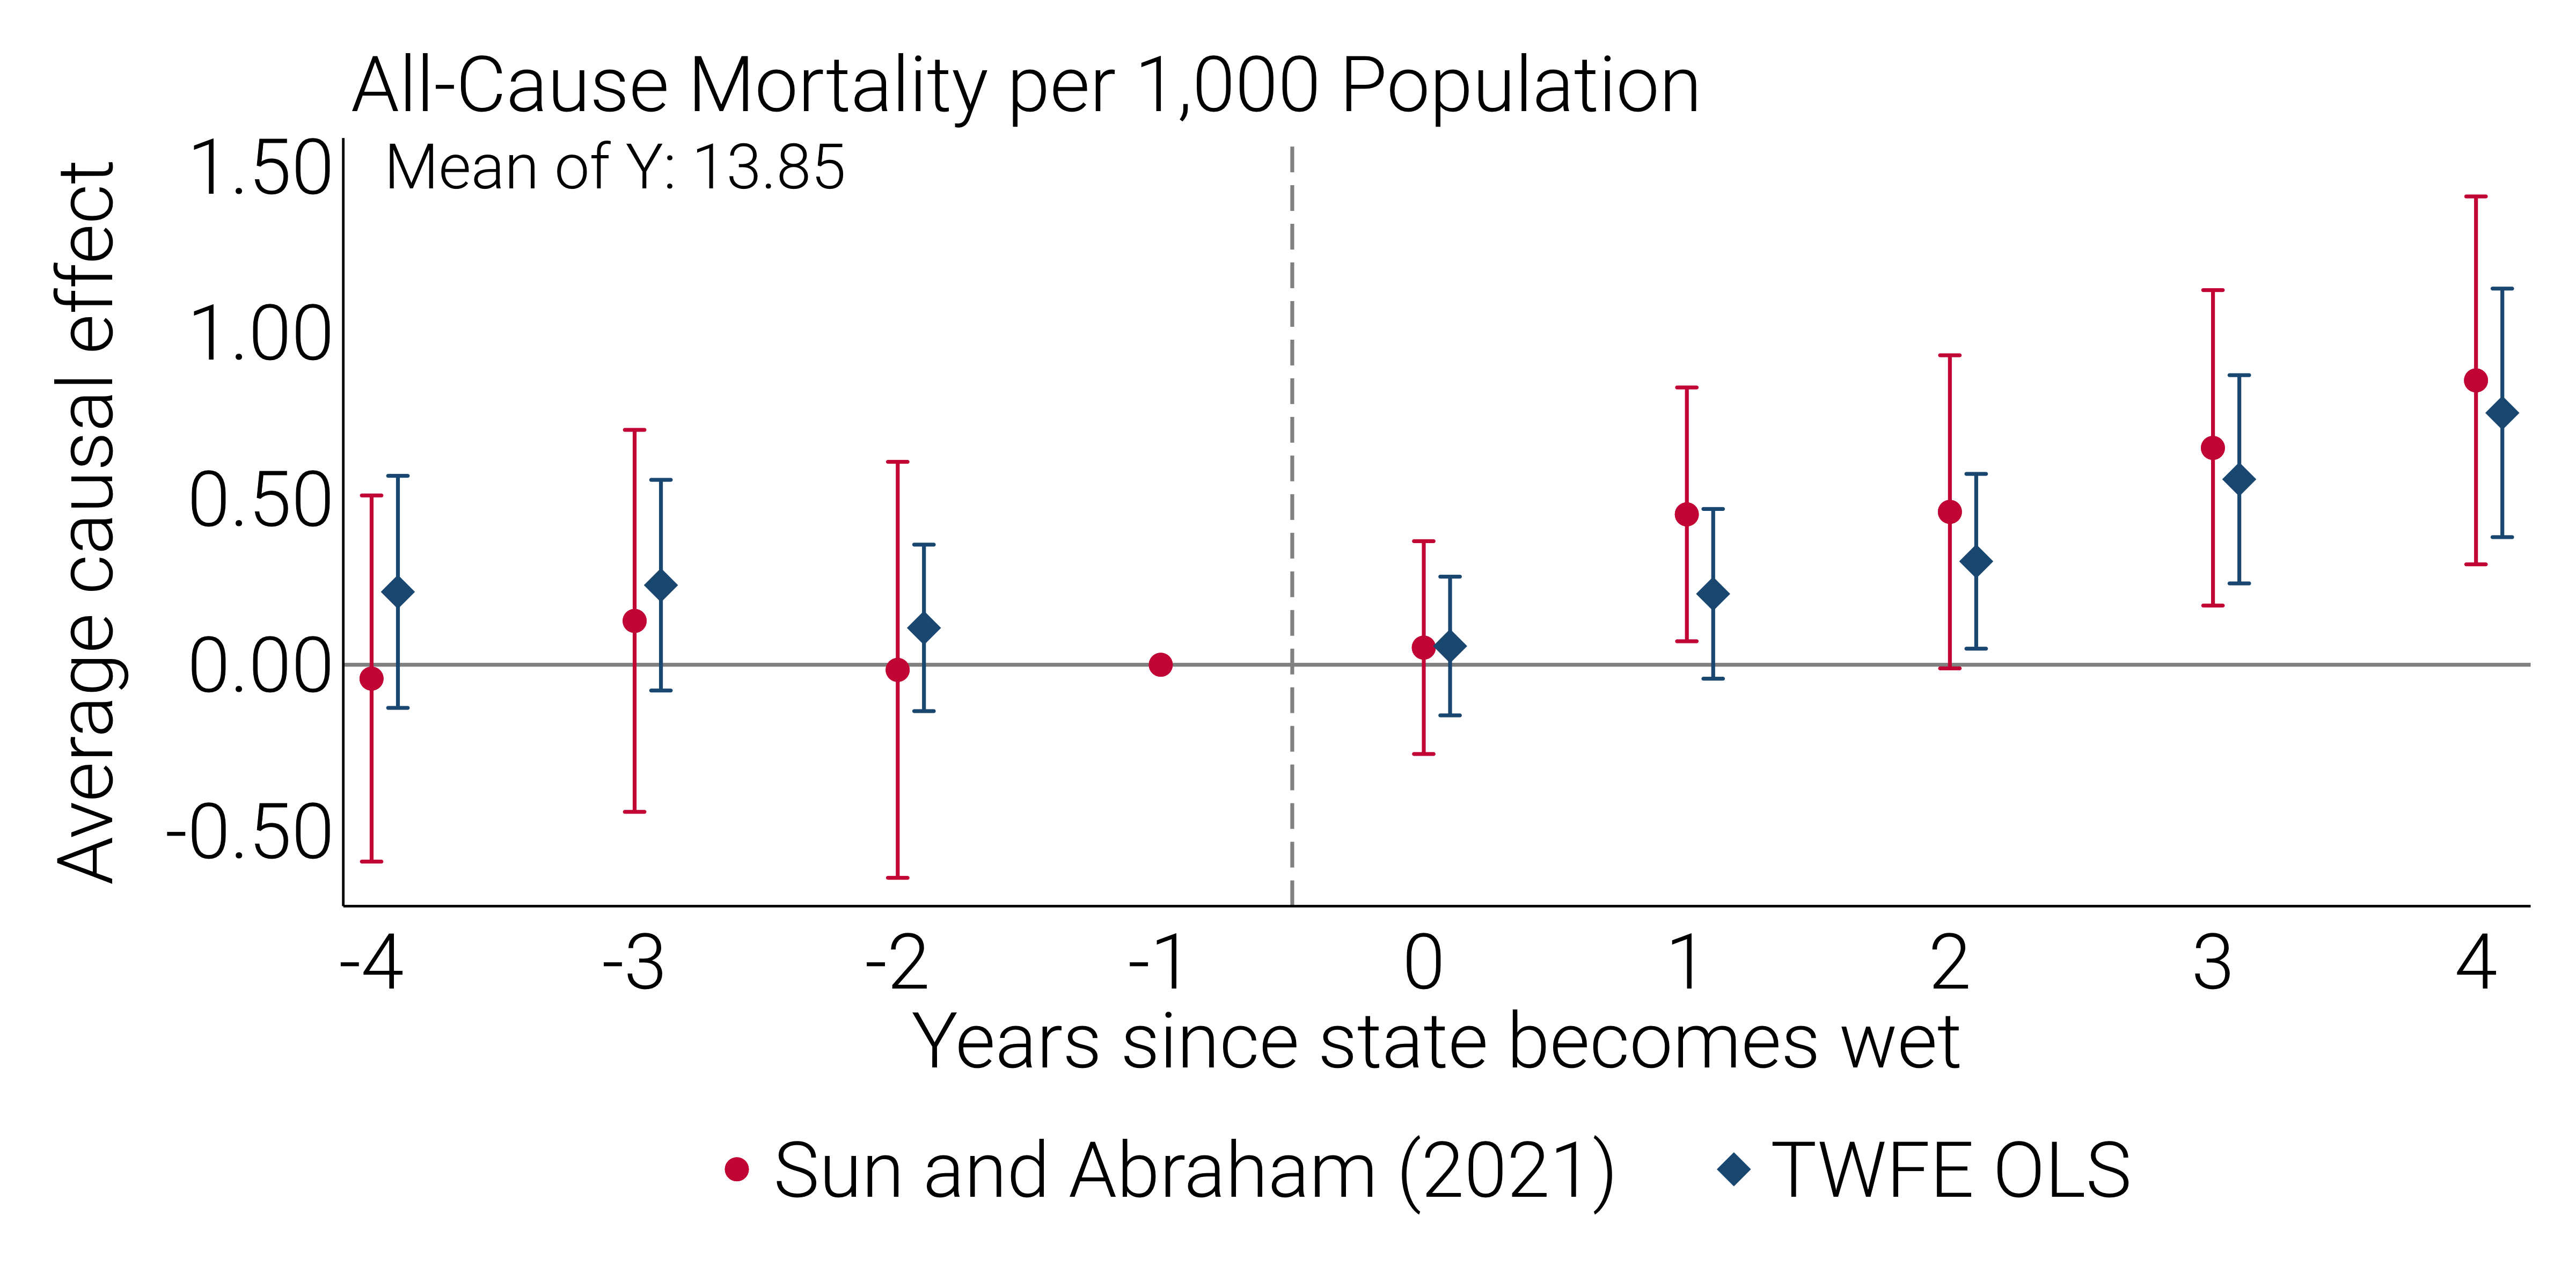
\includegraphics[width=1.0\linewidth]{../analysis/output/appendix/figure_b1a_es_extended_panel_deaths.png}
    \end{subfigure}
    \begin{subfigure}{0.49\linewidth}
        \centering 
        \caption[Heart Disease]{Heart Disease}        
        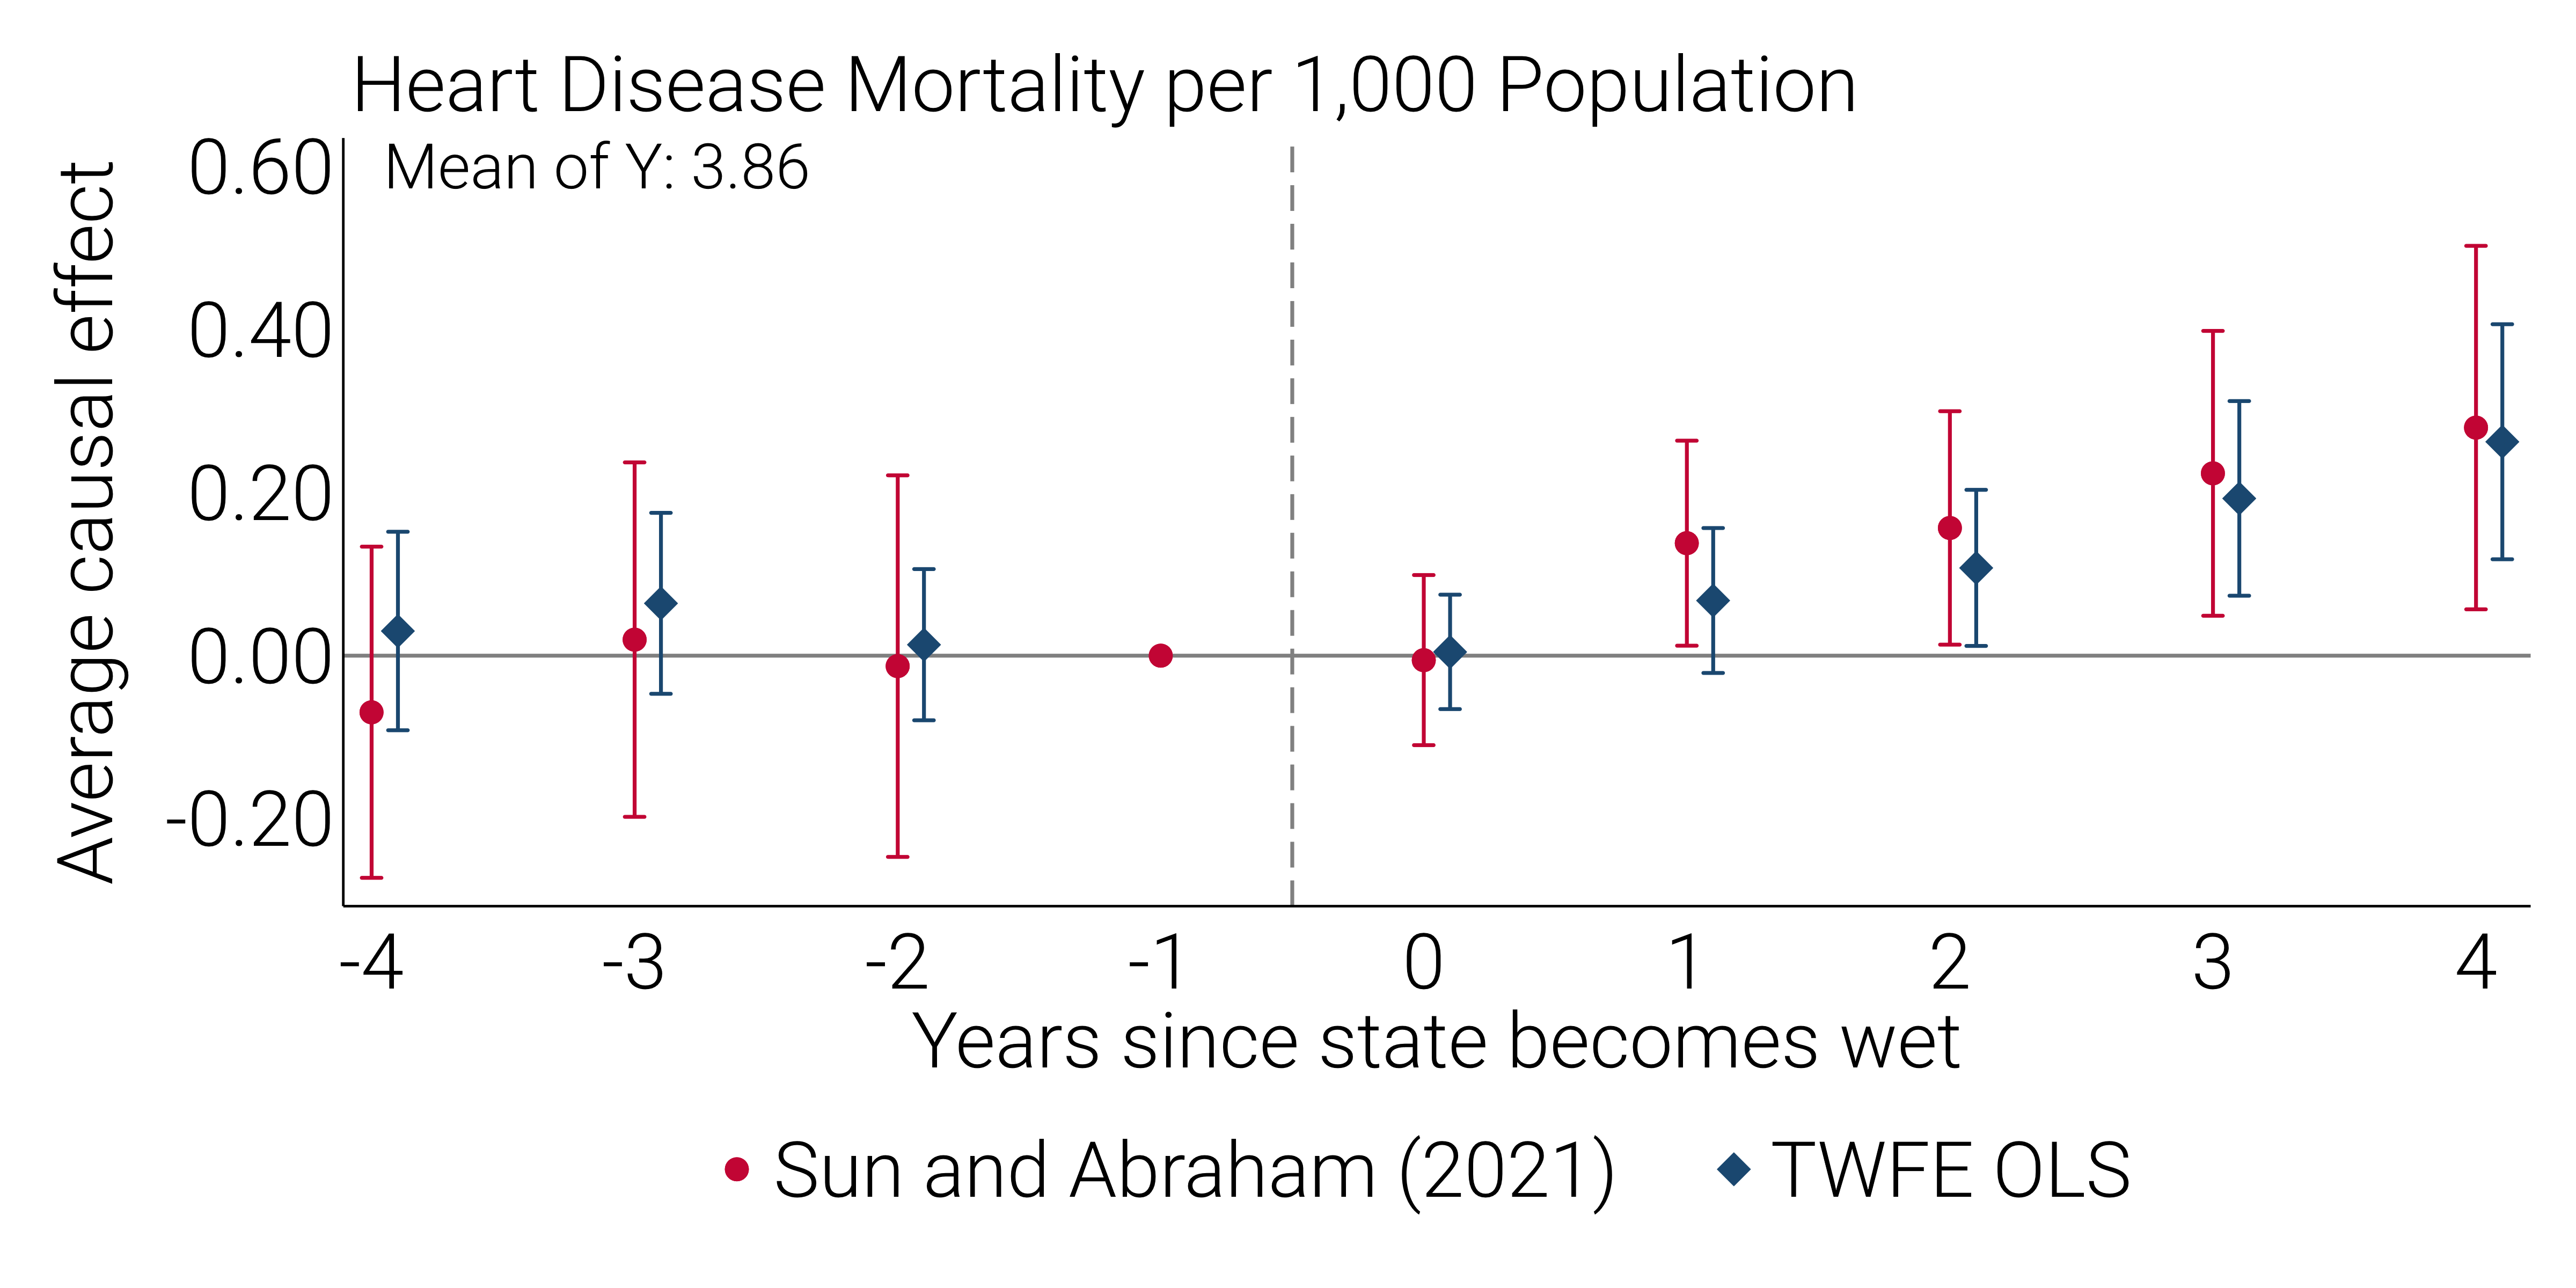
\includegraphics[width=1.0\linewidth]{../analysis/output/appendix/figure_b1b_es_extended_panel_heart.png}
    \end{subfigure}
    \begin{subfigure}{0.49\linewidth}
        \centering 
        \caption[Stroke]{Stroke}        
        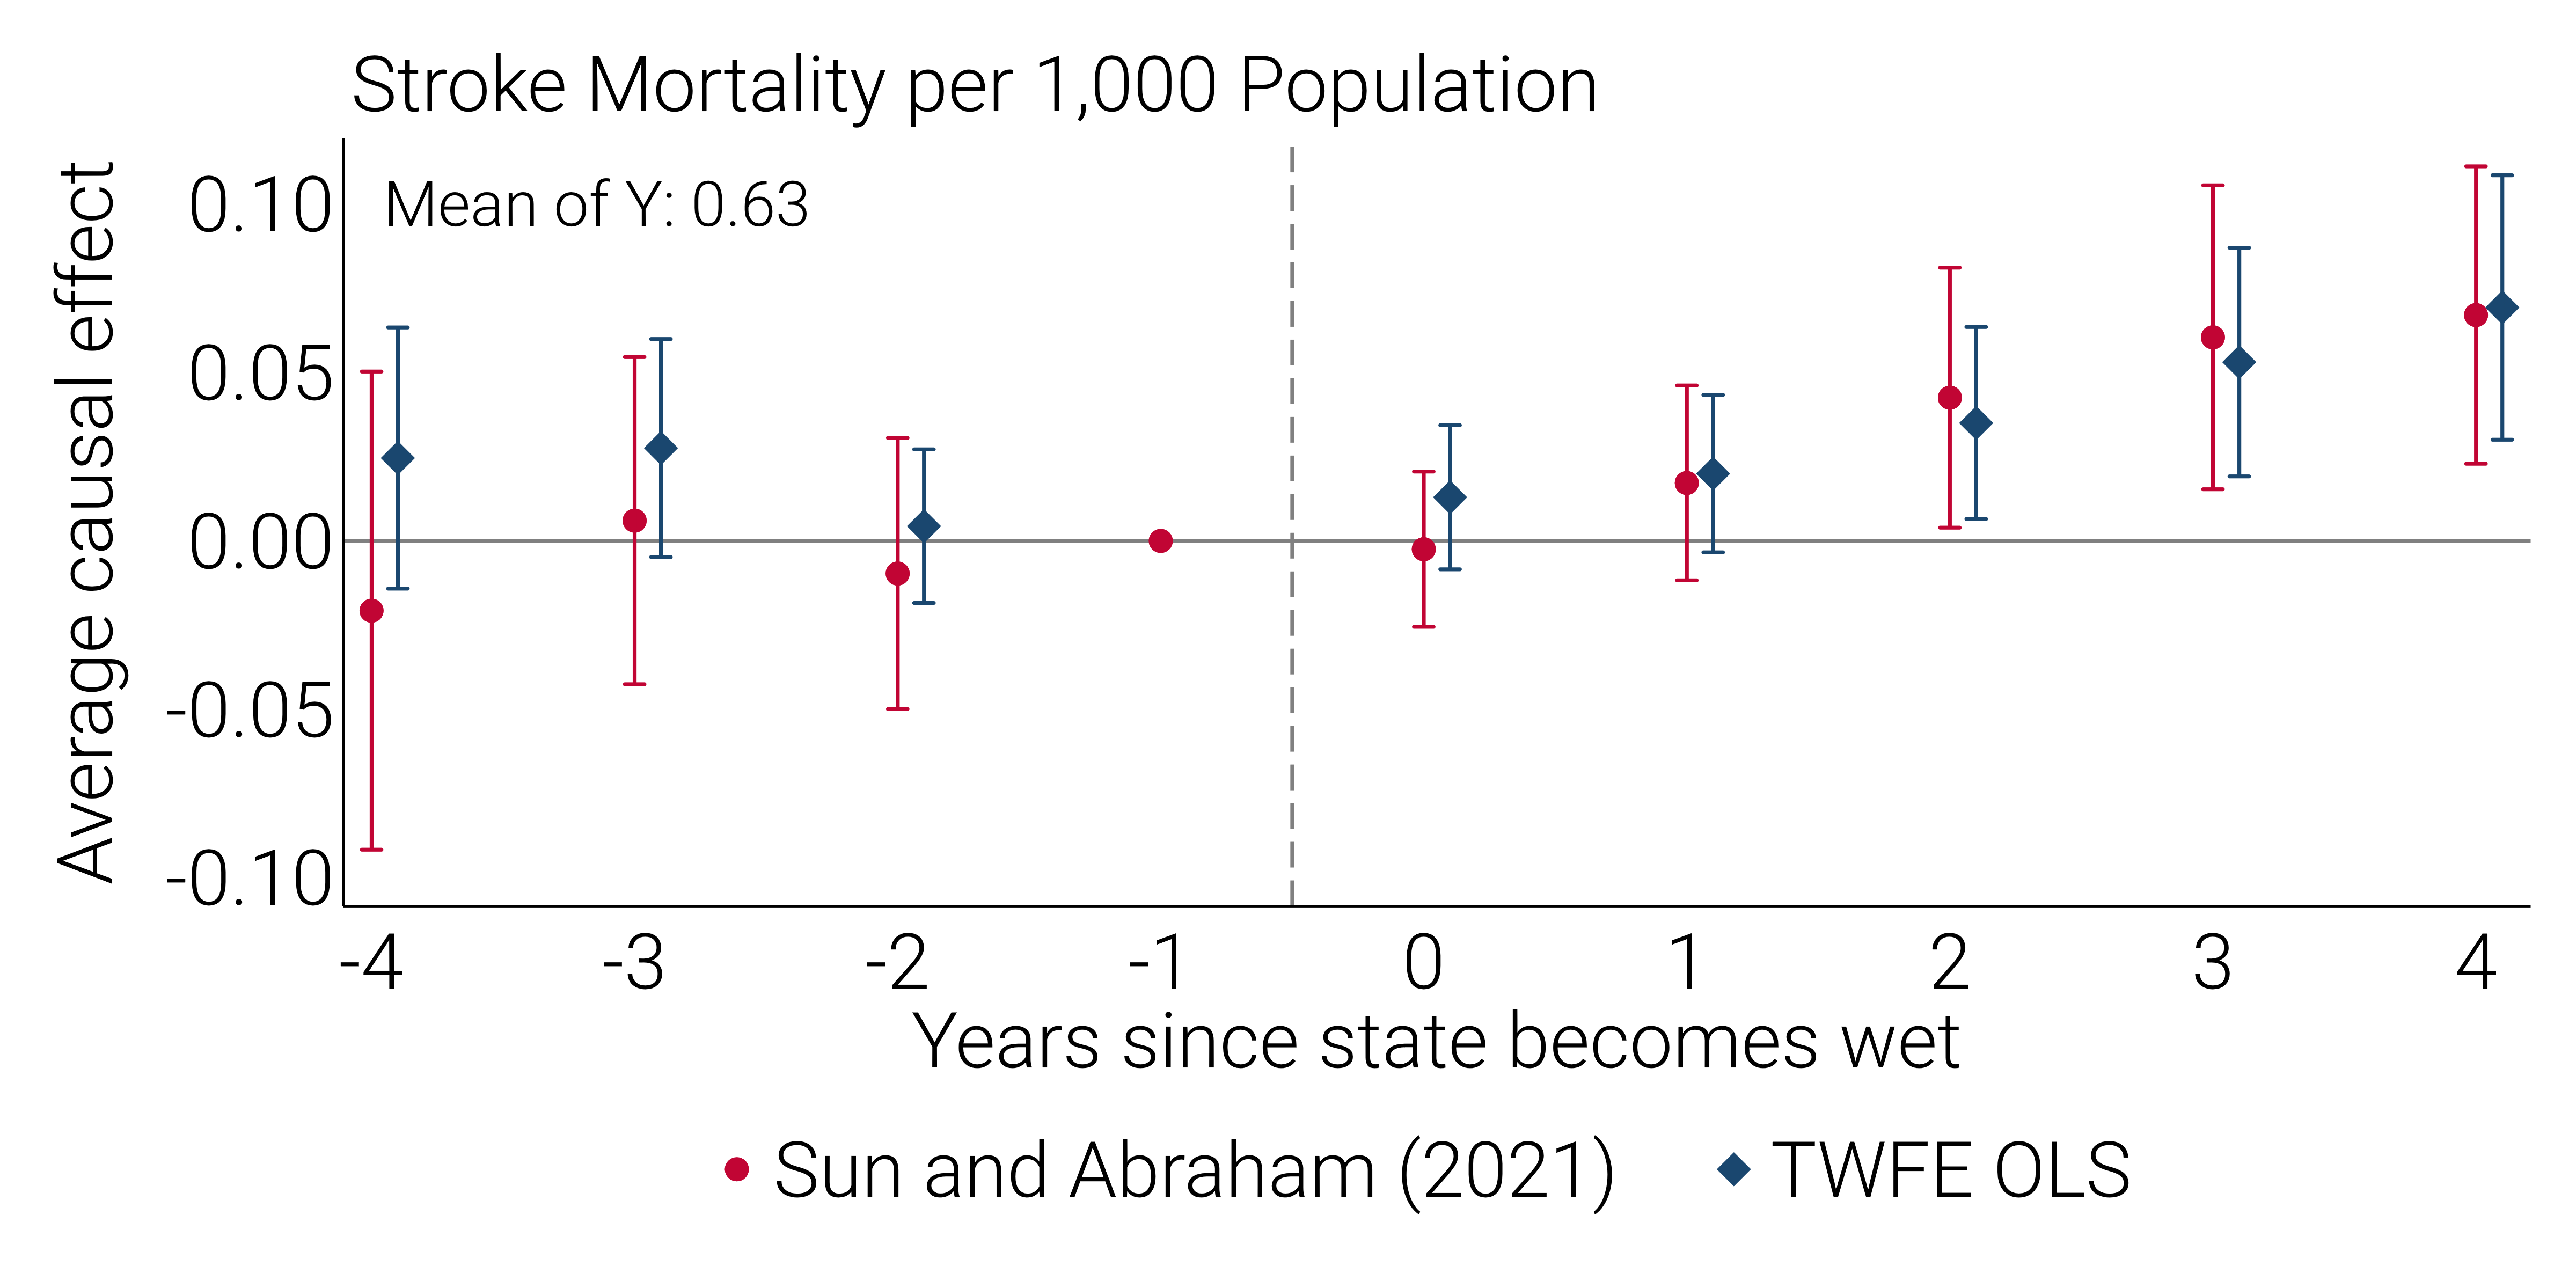
\includegraphics[width=1.0\linewidth]{../analysis/output/appendix/figure_b1c_es_extended_panel_stroke.png}
    \end{subfigure}    
    \begin{subfigure}{0.49\linewidth}
        \centering 
        \caption[Cancer]{Cancer}        
        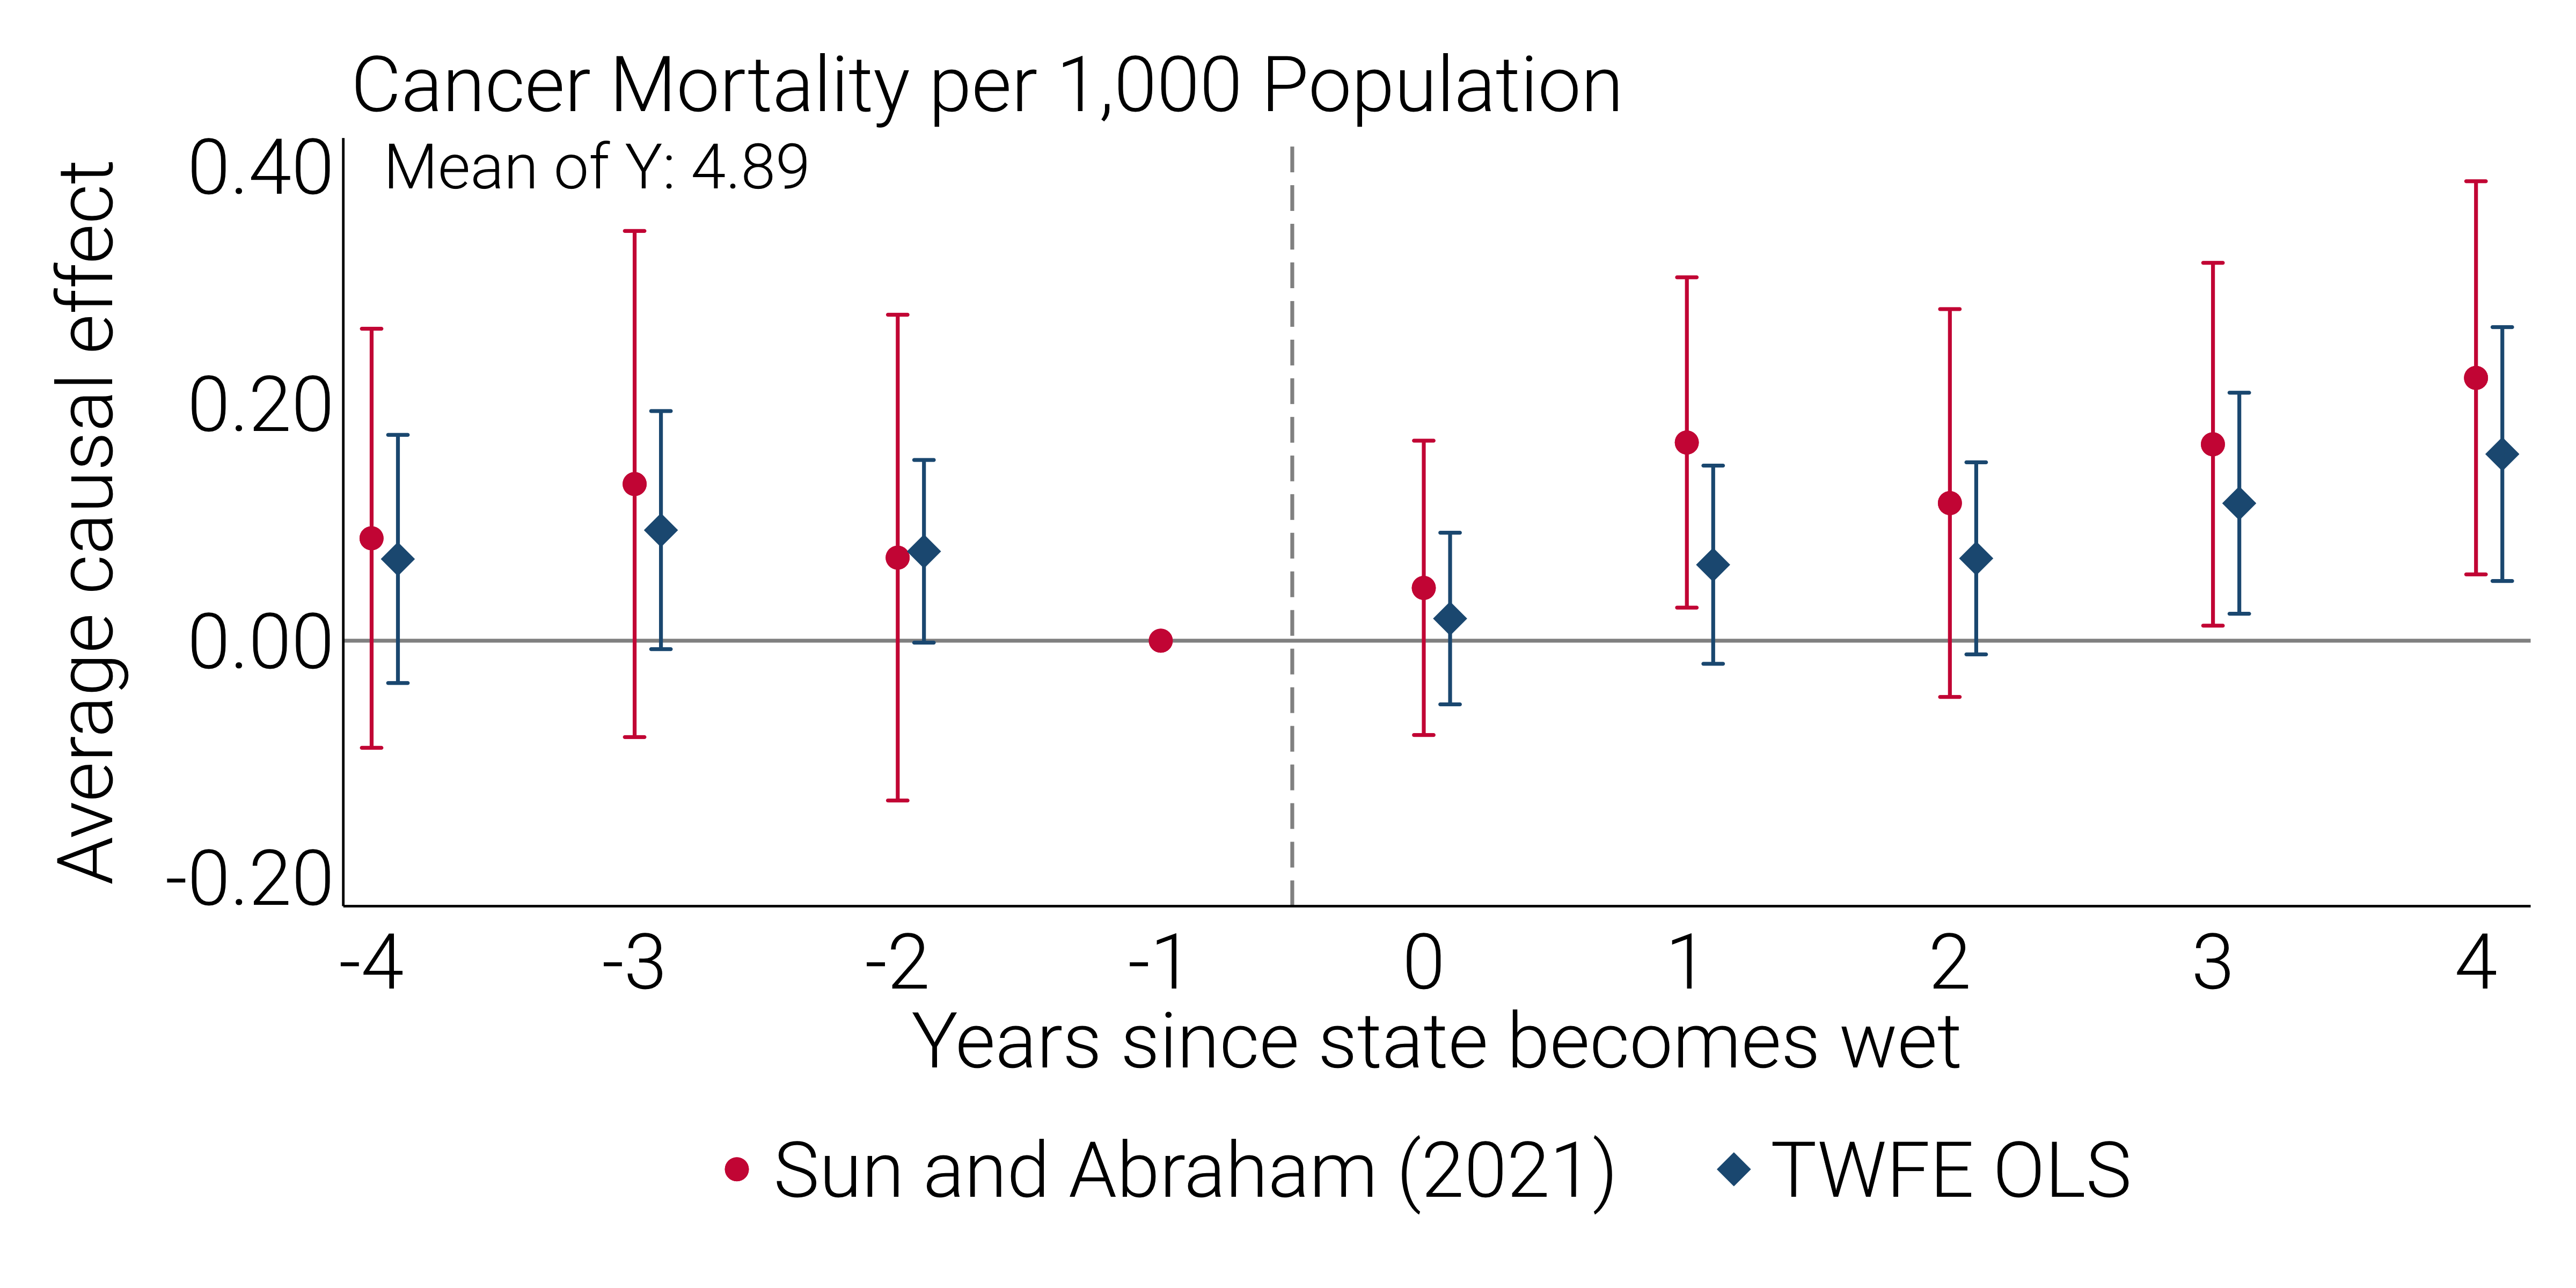
\includegraphics[width=1.0\linewidth]{../analysis/output/appendix/figure_b1d_es_extended_panel_cancer.png}
    \end{subfigure}
    \Fnote{
        Each panel displays event studies with all-cause mortality (panel A) or cause-specific mortality per 1,000 population as the dependent variable (heart disease in panel B, stroke in panel C, and cancer in panel D). 
        Mortality is observed between 1979 and 2004. 
        In all other respects, the clustering, estimation techniques, observation weighting, and specification correspond to those used in Figure~\ref{fig:event-study-cause-of-death}. 
        See the note to Appendix Figure~\ref{fig:event-study-cause-of-death-robust-control} for more details. 
    }
    \label{fig:event-study-cause-of-death-mortality-from-1979}
\end{figure}
\end{landscape}
\restoregeometry

\setcounter{table}{0}\renewcommand{\thetable}{\ref{sec:app-extend-panel}\arabic{table}}
% Table B1: By Cause of Death in Extended Panel
\begin{table}[!ht]\centering
  \begin{adjustbox}{width=1.0\textwidth}
  \centering
    \begin{threeparttable}
     \caption{Aggregate Event Study Estimates for Cause-Specific Mortality}
     \estauto{../analysis/output/appendix/table_b1_extended_panel.tex}{4}{S[table-format=2.3,table-column-width=20mm, table-alignment = center]}
      \label{tab:did-extended-panel}
      \Fignote{
            The dependent variable is the number of all-cause deaths per 1,000 population (Column 1) or the number of cause-specific deaths from heart disease (Column 2), stroke (Column 3), or cancer (Column 4) per 1,000 population. 
            Each coefficient is the average of the \citeApp{sun_estimating_2021} event study coefficients from $l = 0$ to $l = 4$ and represents the average change in the later-life all-cause mortality rate attributable to in utero exposure to the first five years of federal prohibition’s repeal. 
            Mortality is observed between 1979 and 2004. 
            In all other respects, the clustering, estimation techniques, observation weighting, and specification correspond to those used in Figure~\ref{fig:event-study-cause-of-death}. 
            See the note to Appendix Figure~\ref{fig:event-study-cause-of-death-robust-control} for more details. 
            See Table~\ref{tab:icd-crosswalk} in Appendix~\ref{sec:additional-tab-fig} for the crosswalk of ICD9 and ICD10 codes used to construct cause-specific mortality rates.
        }
    \end{threeparttable}
   \end{adjustbox}
\end{table}



%----------------------------------------------------%
%       Appendix C: Results from Continuous Treatment
%----------------------------------------------------%

\FloatBarrier
\newpage 
\newgeometry{top = 0.75in, bottom = 0.75in, right = 0.75in, left = 0.75in, footskip = 0.0in}

\section[Results from Continuous Treatment]{Results from Continuous Treatment\label{sec:app-continuous}}
\setcounter{table}{0}\renewcommand{\thetable}{\ref{sec:app-continuous}\arabic{table}}
\setcounter{figure}{0}\renewcommand{\thefigure}{\ref{sec:app-continuous}\arabic{figure}}

% Figure C1 - Map of county-level variation in wet status
\begin{figure}[!ht]
    \caption[County-Level Variation in Timing of Repeal by Year]{County-Level Variation in Timing of Repeal by Year}
    \centering
        \centering
        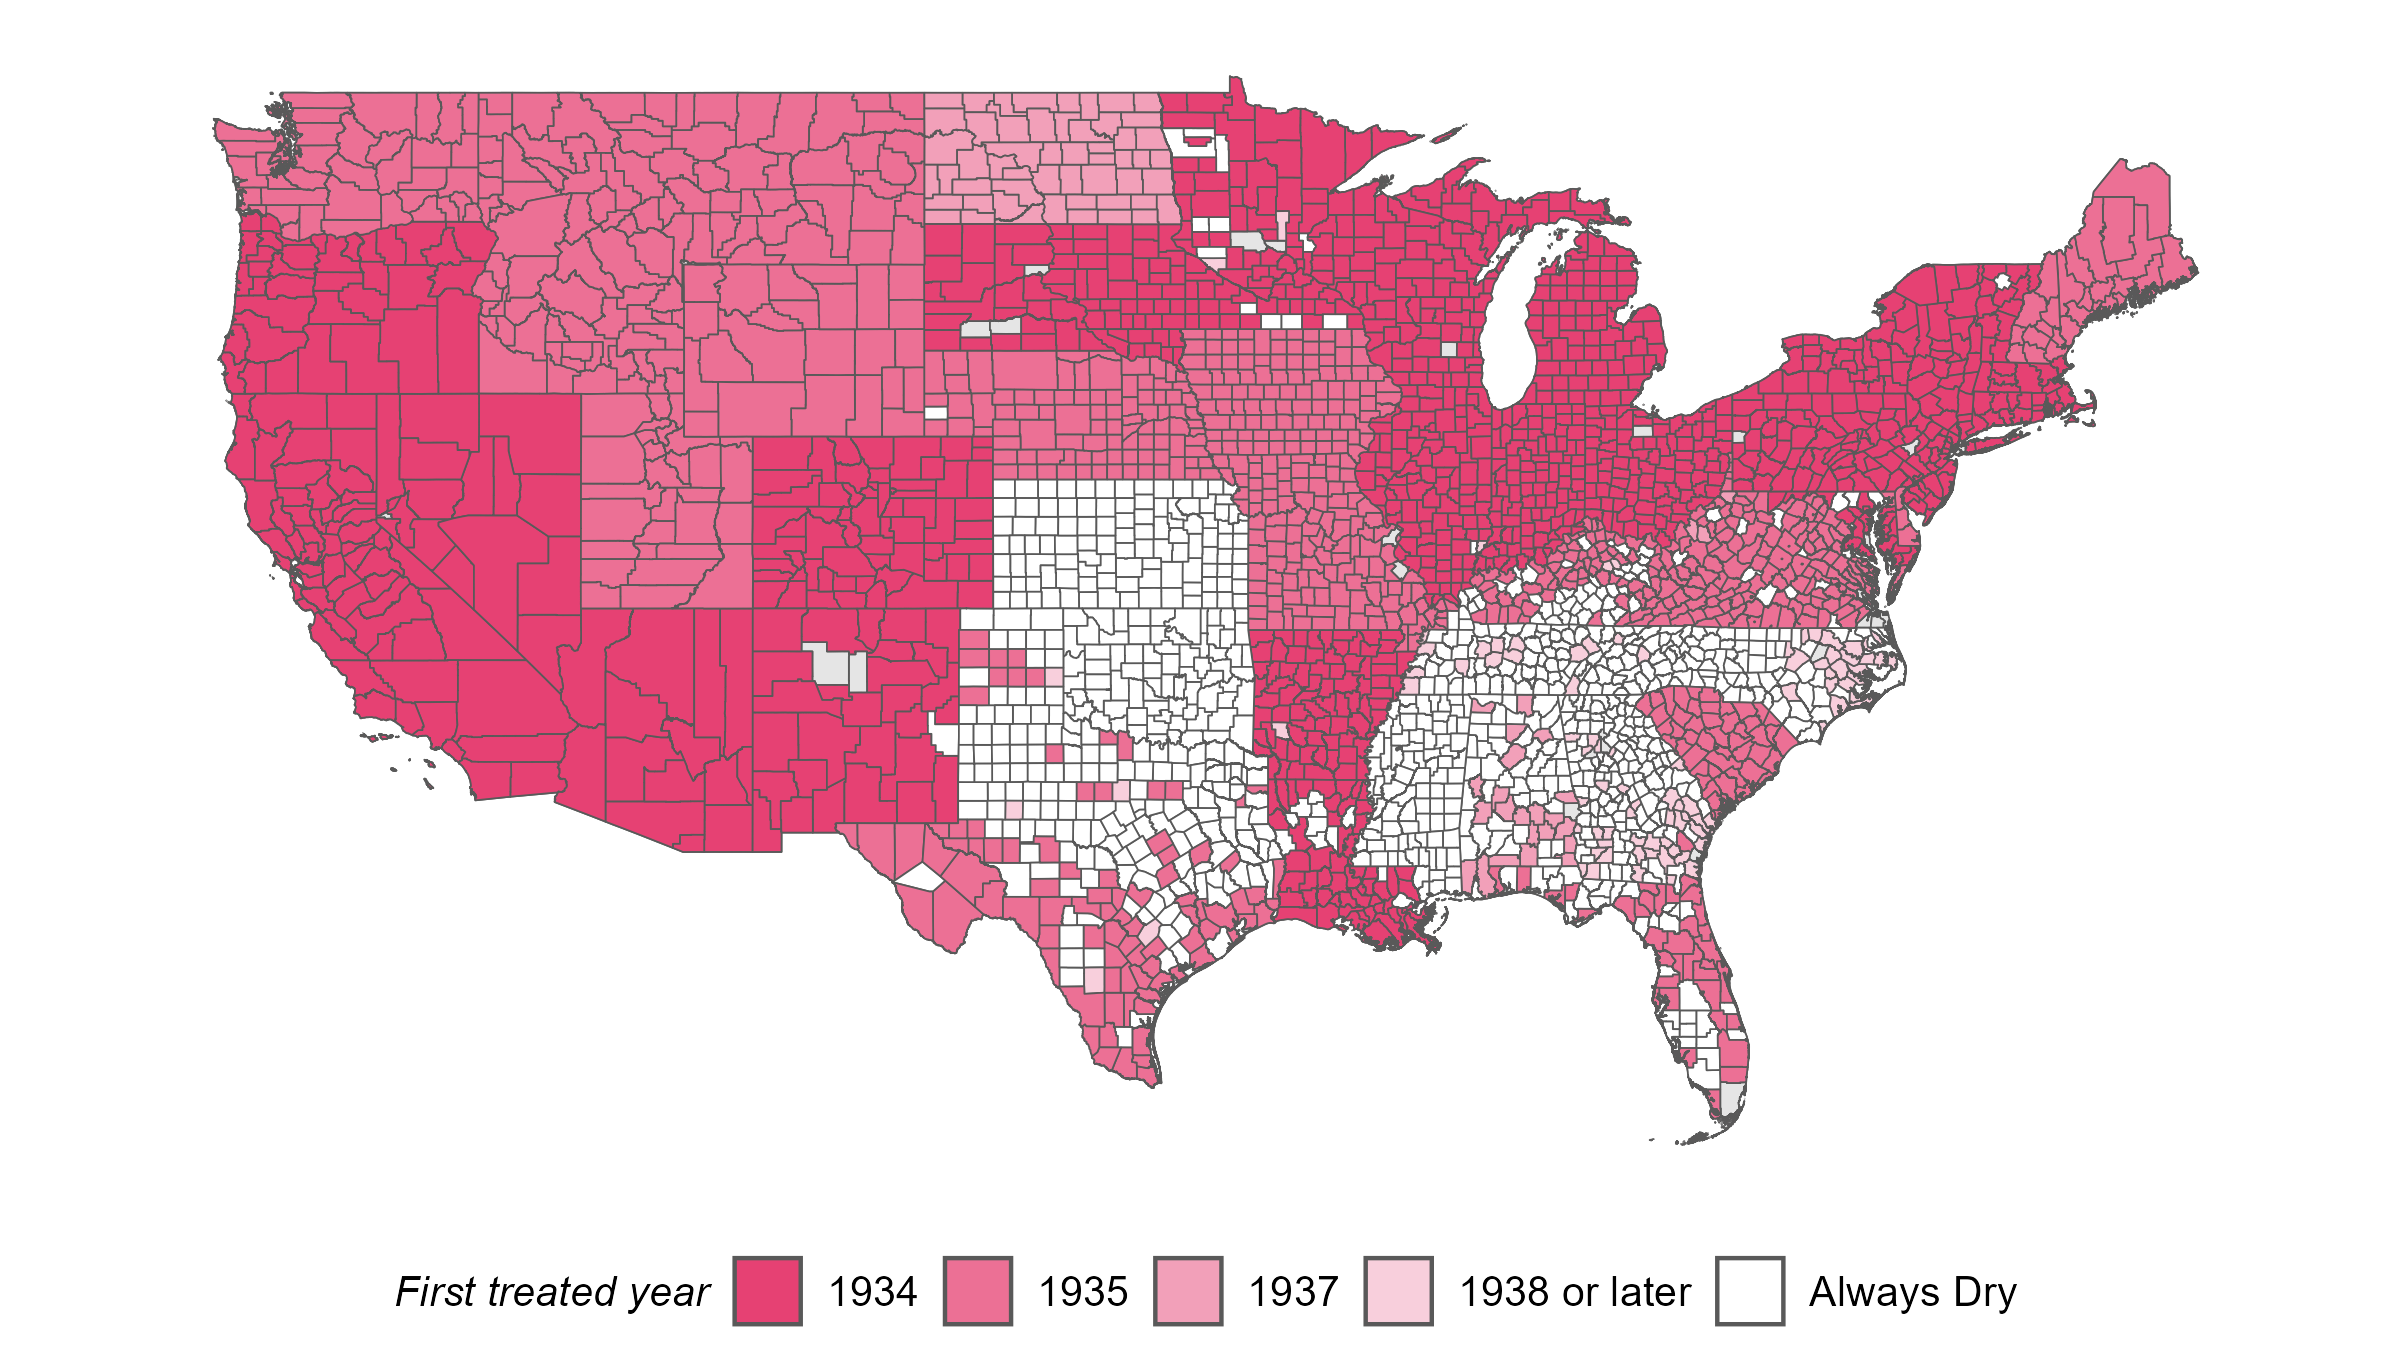
\includegraphics[width=0.8\linewidth]{../analysis/output/appendix/figure_c1_county_wet_map.png}
    \Fnote{{\footnotesize
		This figure displays the initial year when a county turned wet. 
        We group the handful of counties that turned wet in 1940 or 1941 together with counties that turned wet in 1938 to maintain comparability with the variation shown in Panel C of Figure~\ref{fig:descriptive-plots}. 
	}}
    \label{fig:county-wet-map}
\end{figure}


% Figure C2 - Map of continuous variation in wet status
\begin{figure}[!ht]
    \caption[Variation in Share of Population Residing in Wet Counties By State]{Variation in Share of Population Residing in Wet Counties By State}
    \centering
        \centering
        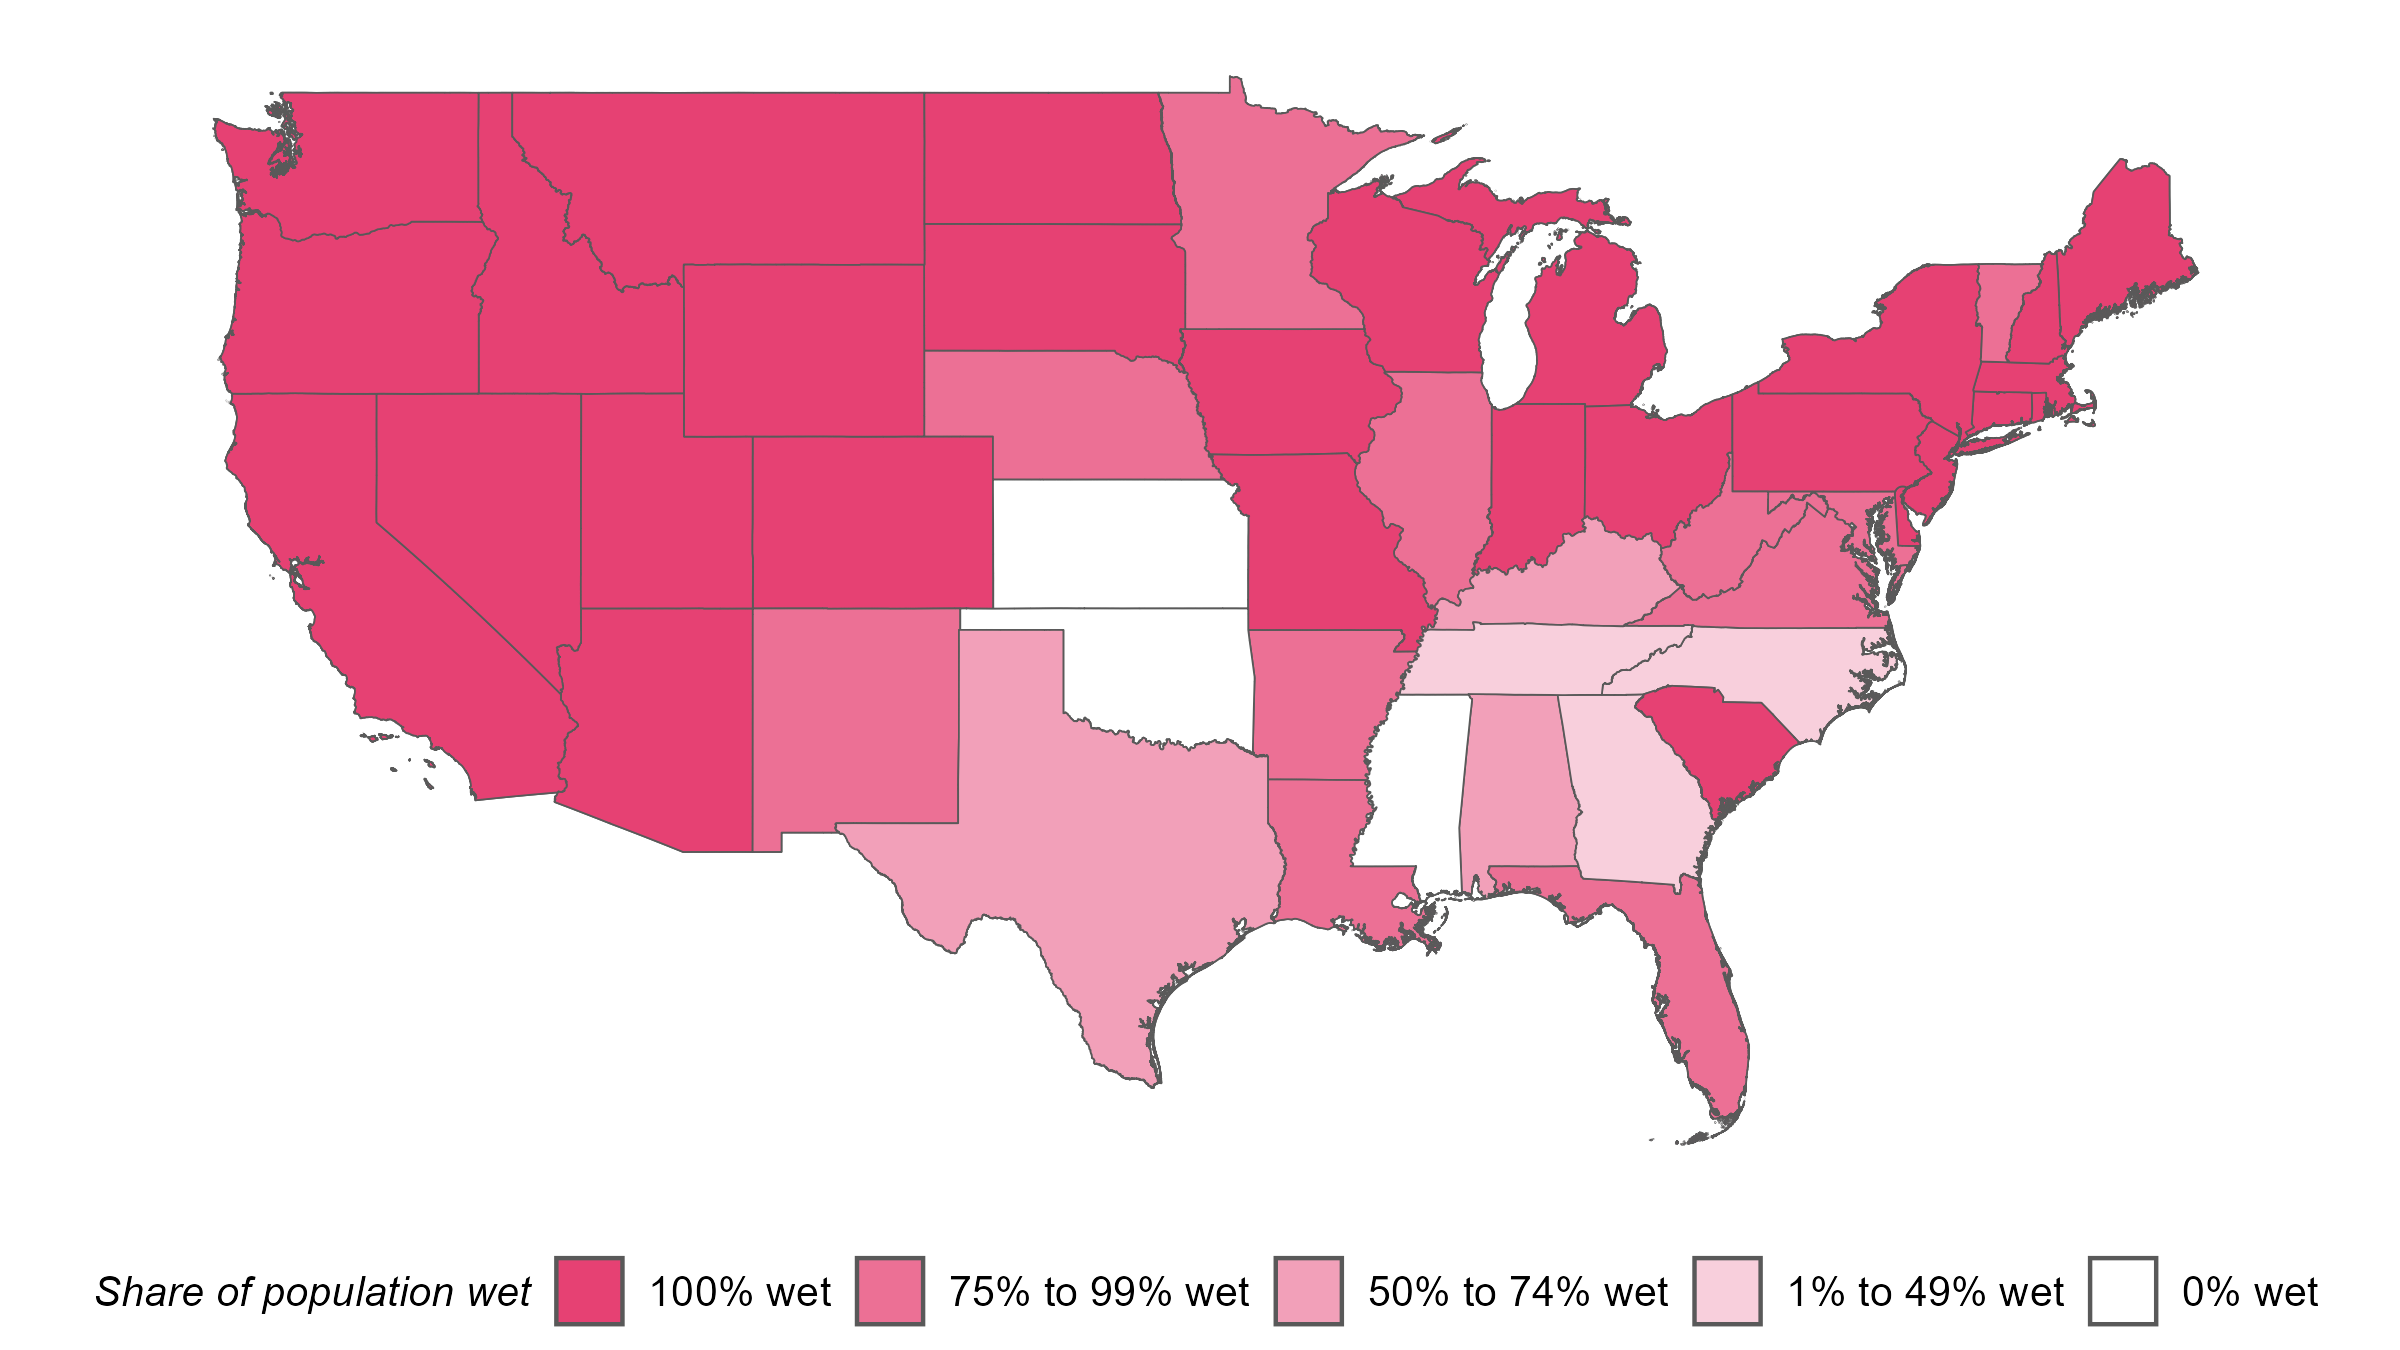
\includegraphics[width=0.8\linewidth]{../analysis/output/appendix/figure_c2_continuous_map.png}
    \Fnote{{\footnotesize
		This figure plots the average share of states' population that is treated (i.e., residing in wet counties) between 1938 and 1941. 
		In the underlying data, this share varies by year-to-year and is used as the treatment in Table~\ref{tab:did-continuous-treatment}.
        Map source: \citeApp{manson_ipums_2020}.
	}}
    \label{fig:continuous-wet-map}
\end{figure}

\restoregeometry

% Table C1: By Cause of Death with Continuous Treatment
\begin{table}[!ht]\centering
  \begin{adjustbox}{width=1.0\textwidth}
  \centering
    \begin{threeparttable}
     \caption{Difference-in-Differences Estimates for Cause-Specific Mortality with Continuous Treatment}
     \estauto{../analysis/output/appendix/table_c1_continuous_treatment.tex}{4}{S[table-format=2.3,table-column-width=20mm, table-alignment = center]}
      \label{tab:did-continuous-treatment}
      \Fignote{
            The dependent variable is the number of deaths per 1,000 population by cause. 
            The treatment variable ``wet status'' measures the share of a state’s population residing in wet counties in the year of birth. 
            Each coefficient is the average of the \citeApp{sun_estimating_2021} event study coefficients from $l = 0$ to $l = 4$ and represents the average change in the later-life all-cause mortality rate attributable to in utero exposure to the first five years of federal prohibition’s repeal. 
            In all other respects, the clustering, estimation techniques, observation weighting, sampling, and specification are the same as in Table~\ref{tab:did-by-cause-of-death}. 
            See the note to Appendix Figure~\ref{fig:event-study-cause-of-death-robust-control} for more details. 
        }
    \end{threeparttable}
   \end{adjustbox}
\end{table}



%----------------------------------------------------%
%       Appendix D: Cumulative Mortality
%----------------------------------------------------%
\setcounter{table}{0}\renewcommand{\thetable}{\ref{sec:cumulative-mortality}\arabic{table}}
\setcounter{figure}{0}\renewcommand{\thefigure}{\ref{sec:cumulative-mortality}\arabic{figure}}

% Figure D1 - Event study - Cumlative All-cause mortality, heart disease, cancer, and stroke
\FloatBarrier
\newpage 
\newgeometry{top = 0.5in, bottom = 0.5in, right = 0.25in, left = 0.5in, footskip = 0.0in}
\begin{landscape}
\section[Results Using Cumulative Mortality]{Results Using Cumulative Mortality\label{sec:cumulative-mortality}}
\begin{figure}[!ht]
    \caption[Cumulative Mortality Event Studies By Cause of Death]{Cumulative Mortality Event Studies By Cause of Death}
    \centering
    \begin{subfigure}{0.47\linewidth}
        \centering 
        \caption[All-Cause Mortality]{All-Cause Mortality}        
        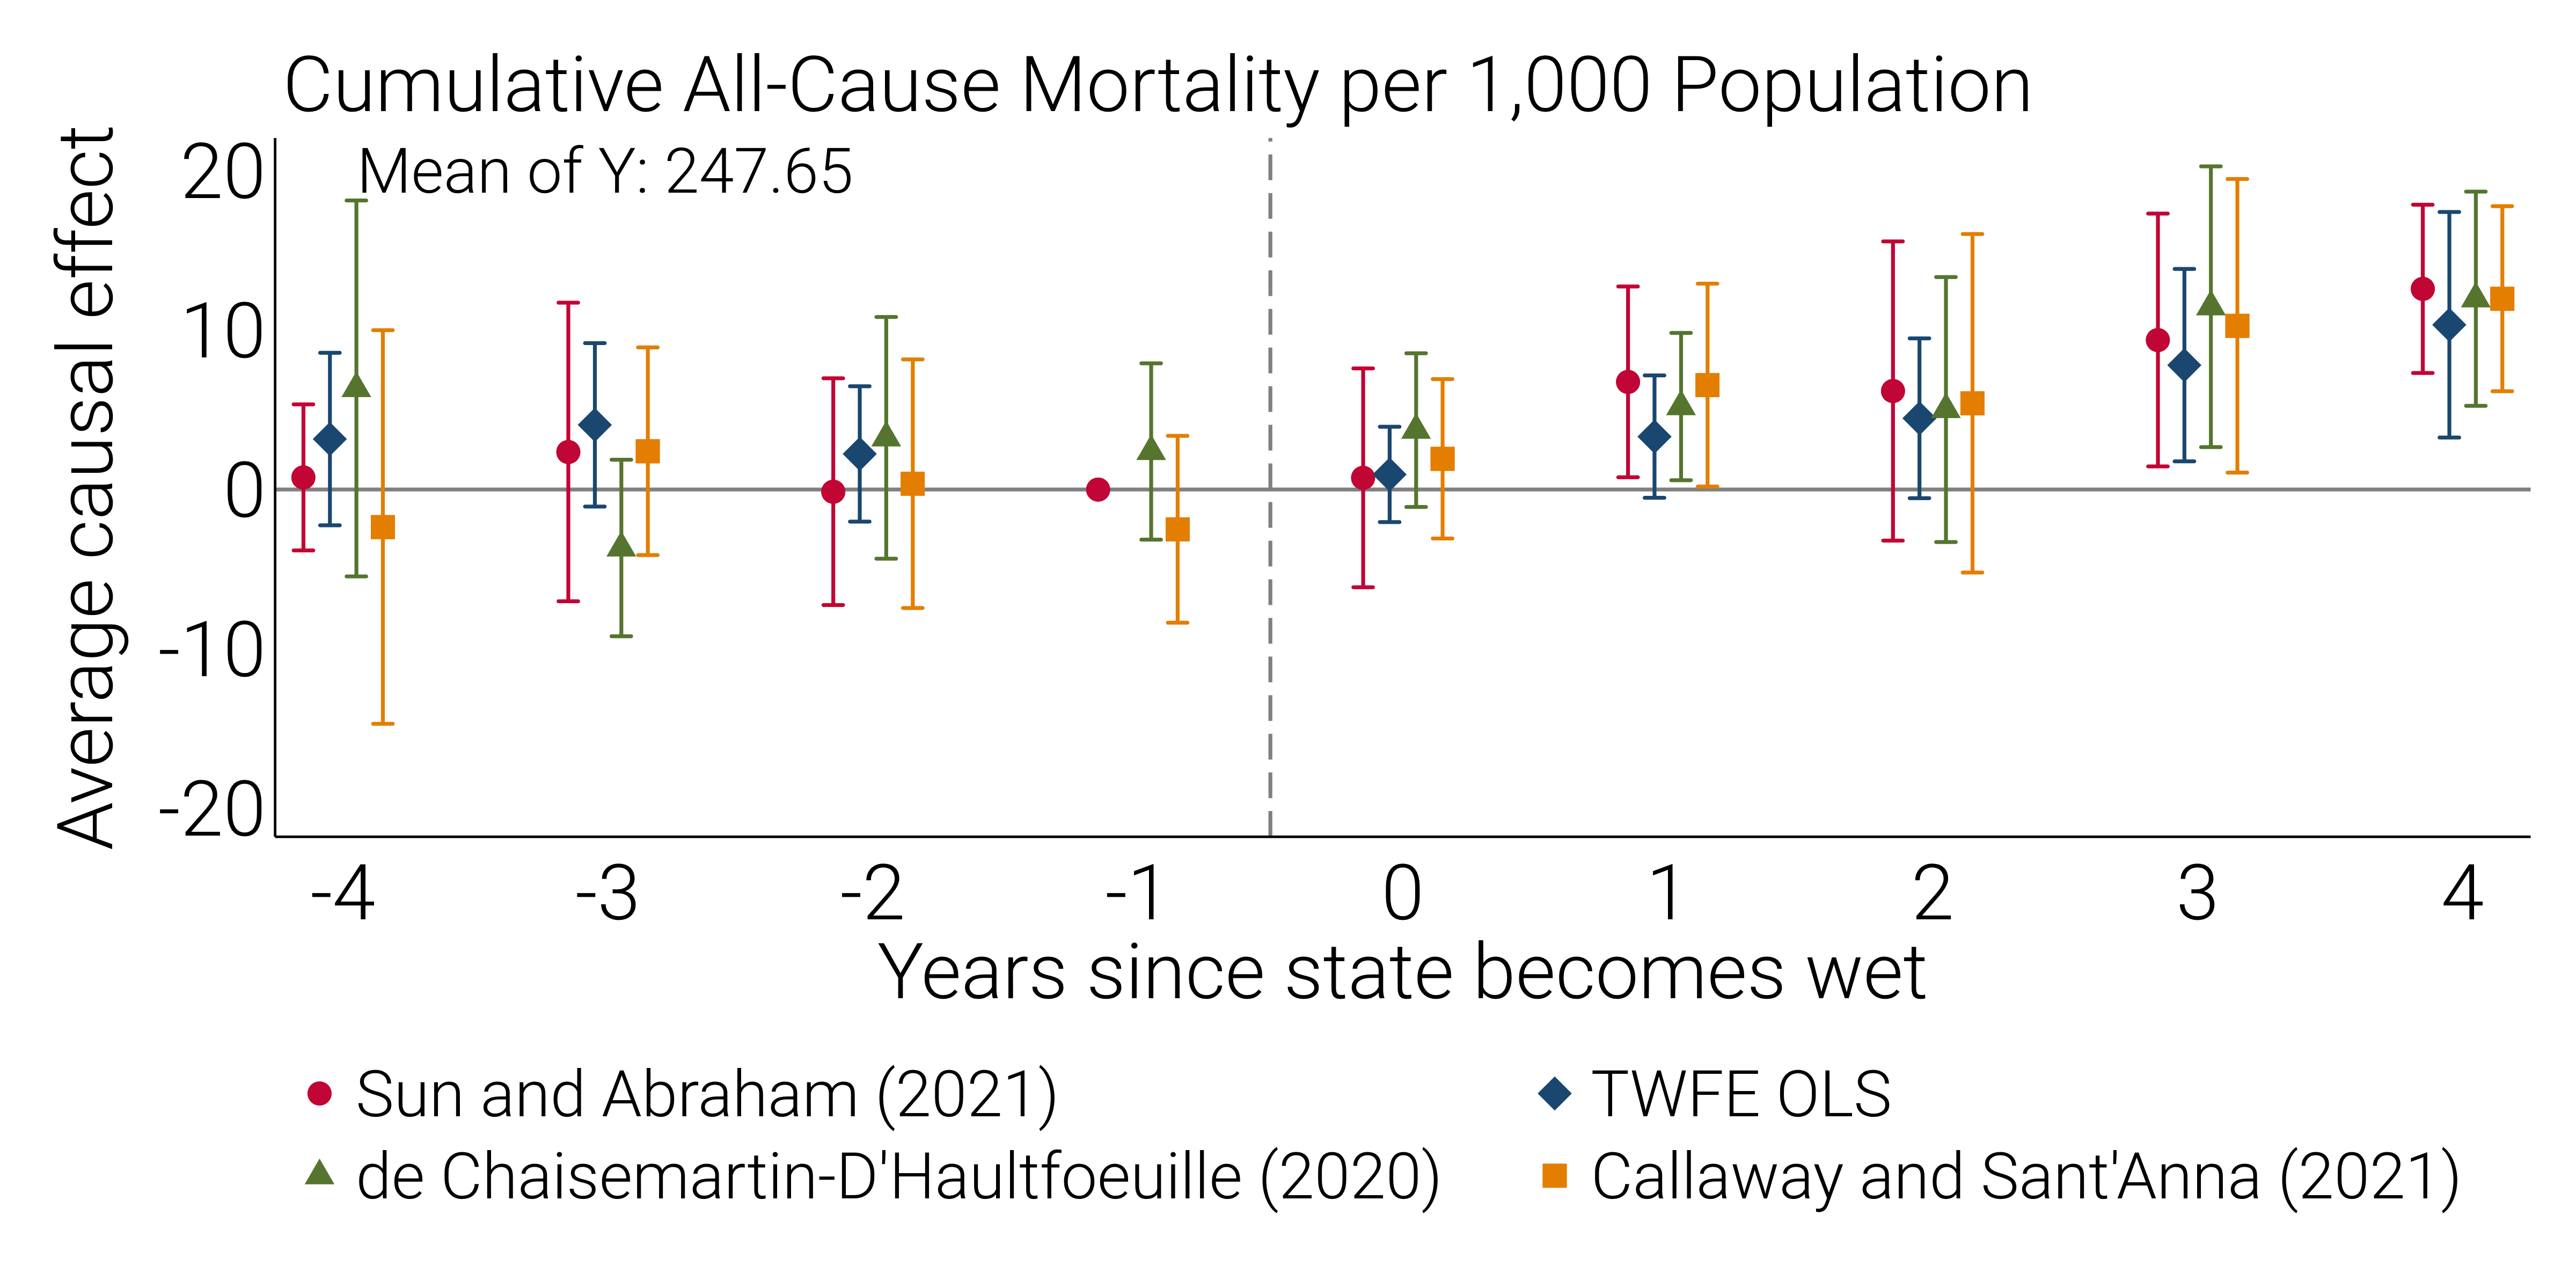
\includegraphics[width=1.0\linewidth]{../analysis/output/appendix/figure_d1a_es_cumulative_deaths.png}
    \end{subfigure}
    \begin{subfigure}{0.47\linewidth}
        \centering 
        \caption[Heart Disease]{Heart Disease}        
        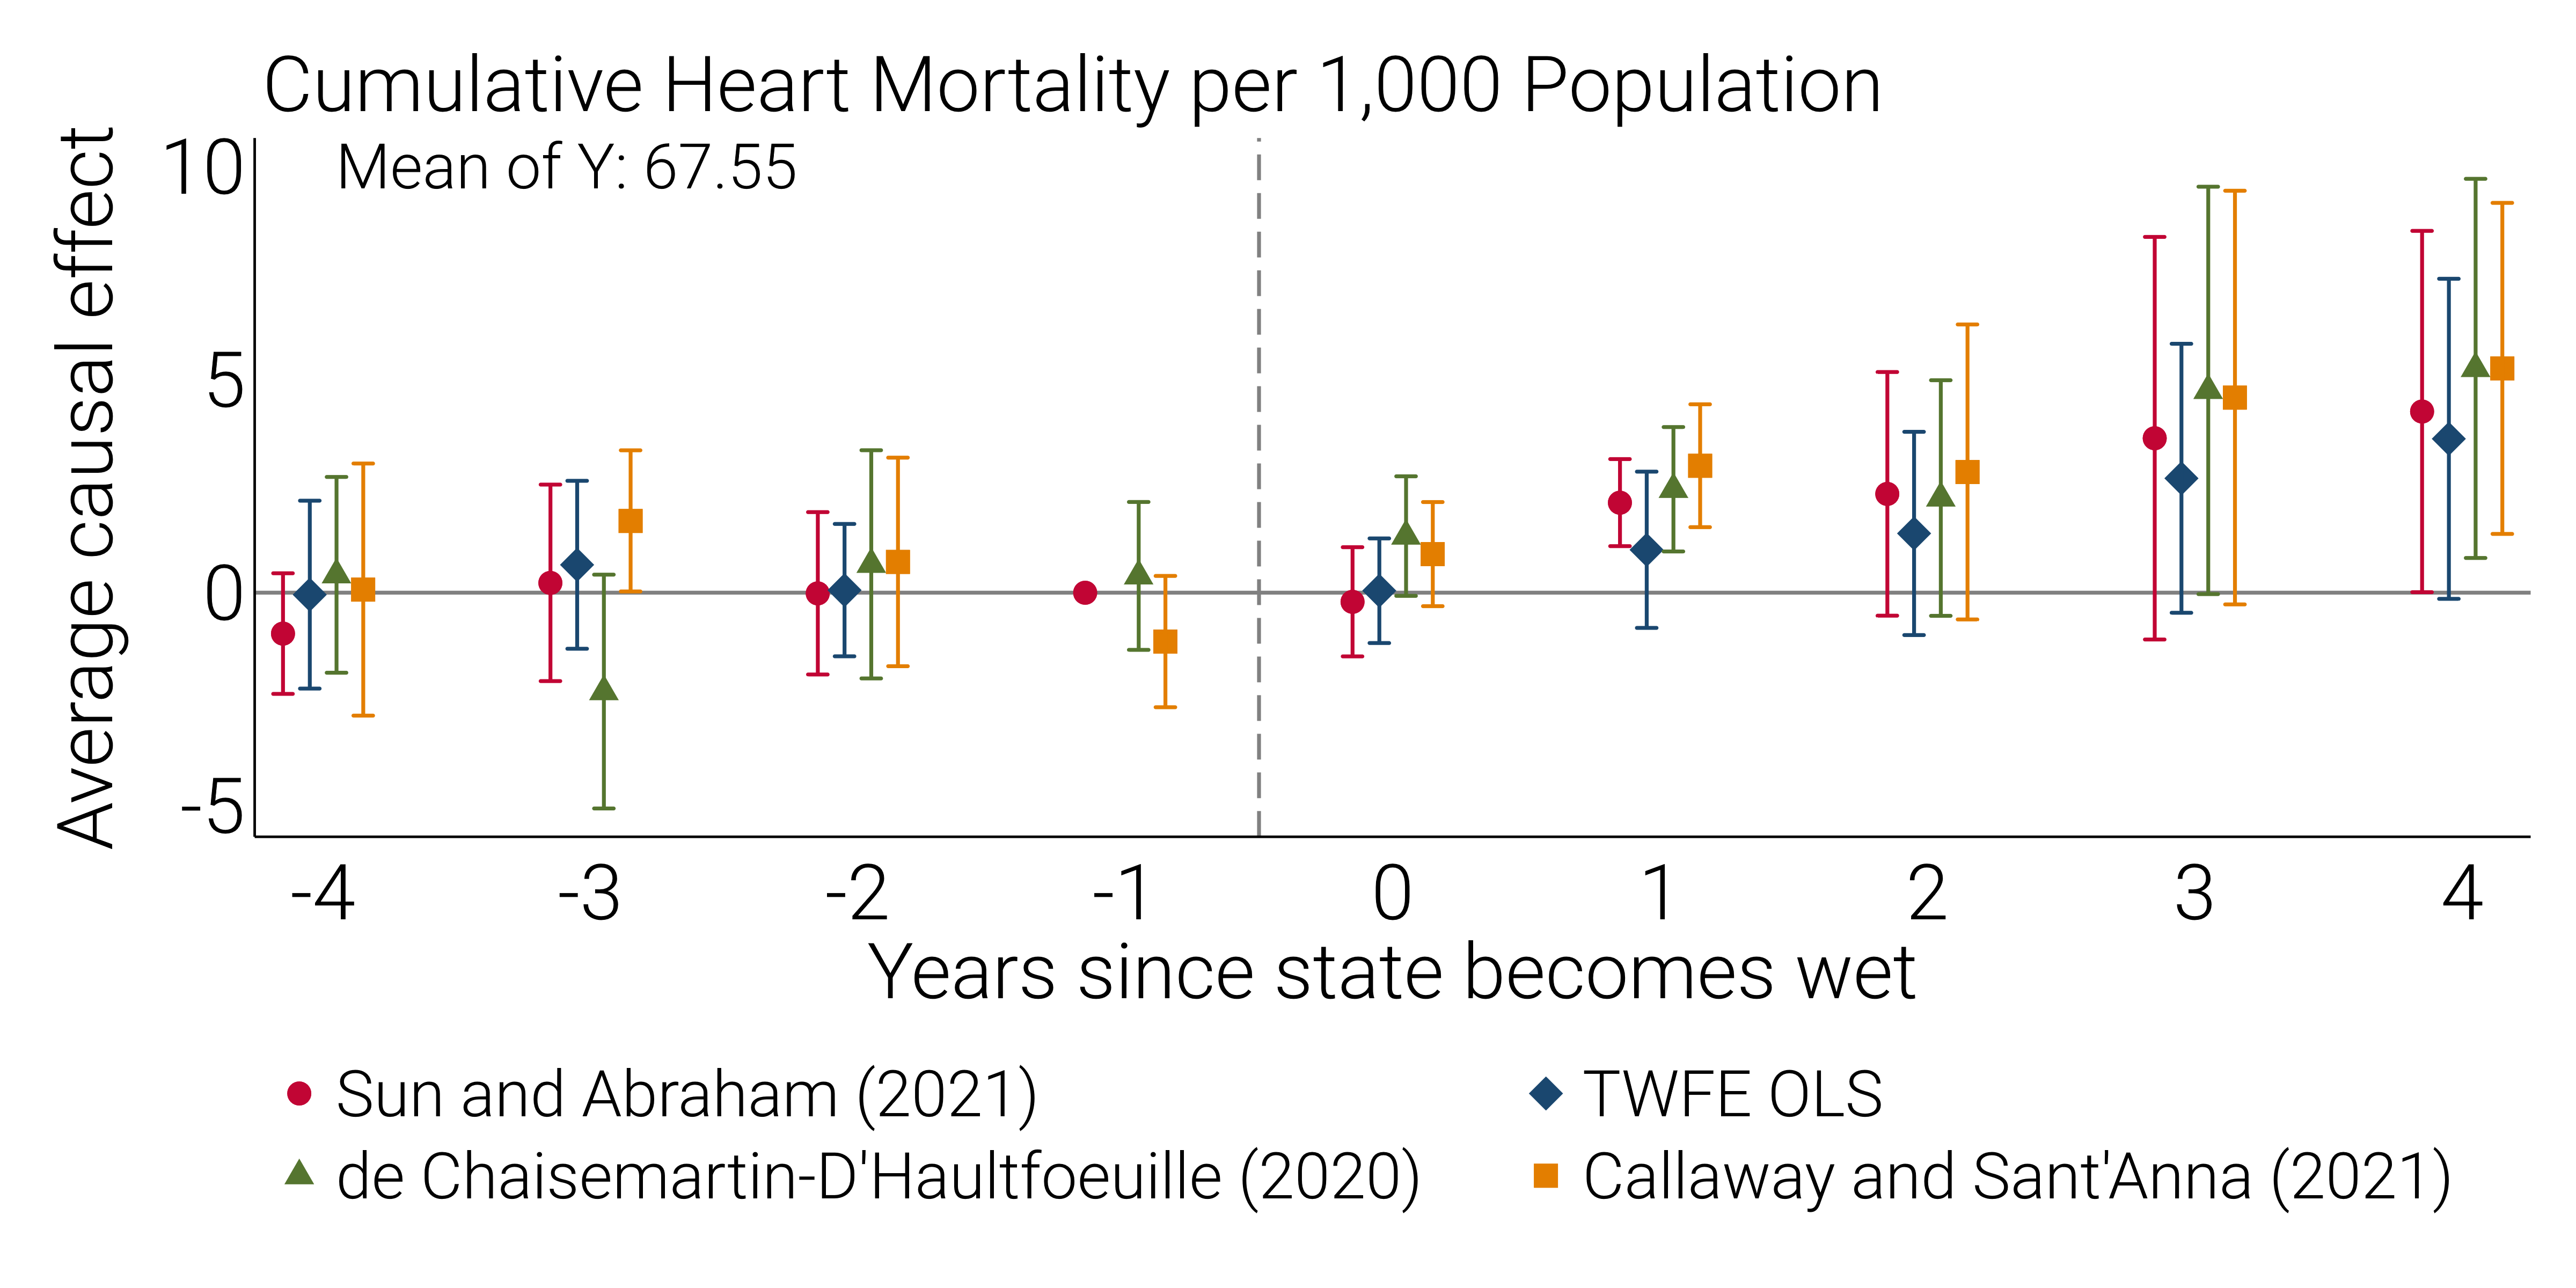
\includegraphics[width=1.0\linewidth]{../analysis/output/appendix/figure_d1b_es_cumulative_heart.png}
    \end{subfigure}
    \begin{subfigure}{0.47\linewidth}
        \centering 
        \caption[Stroke]{Stroke}        
        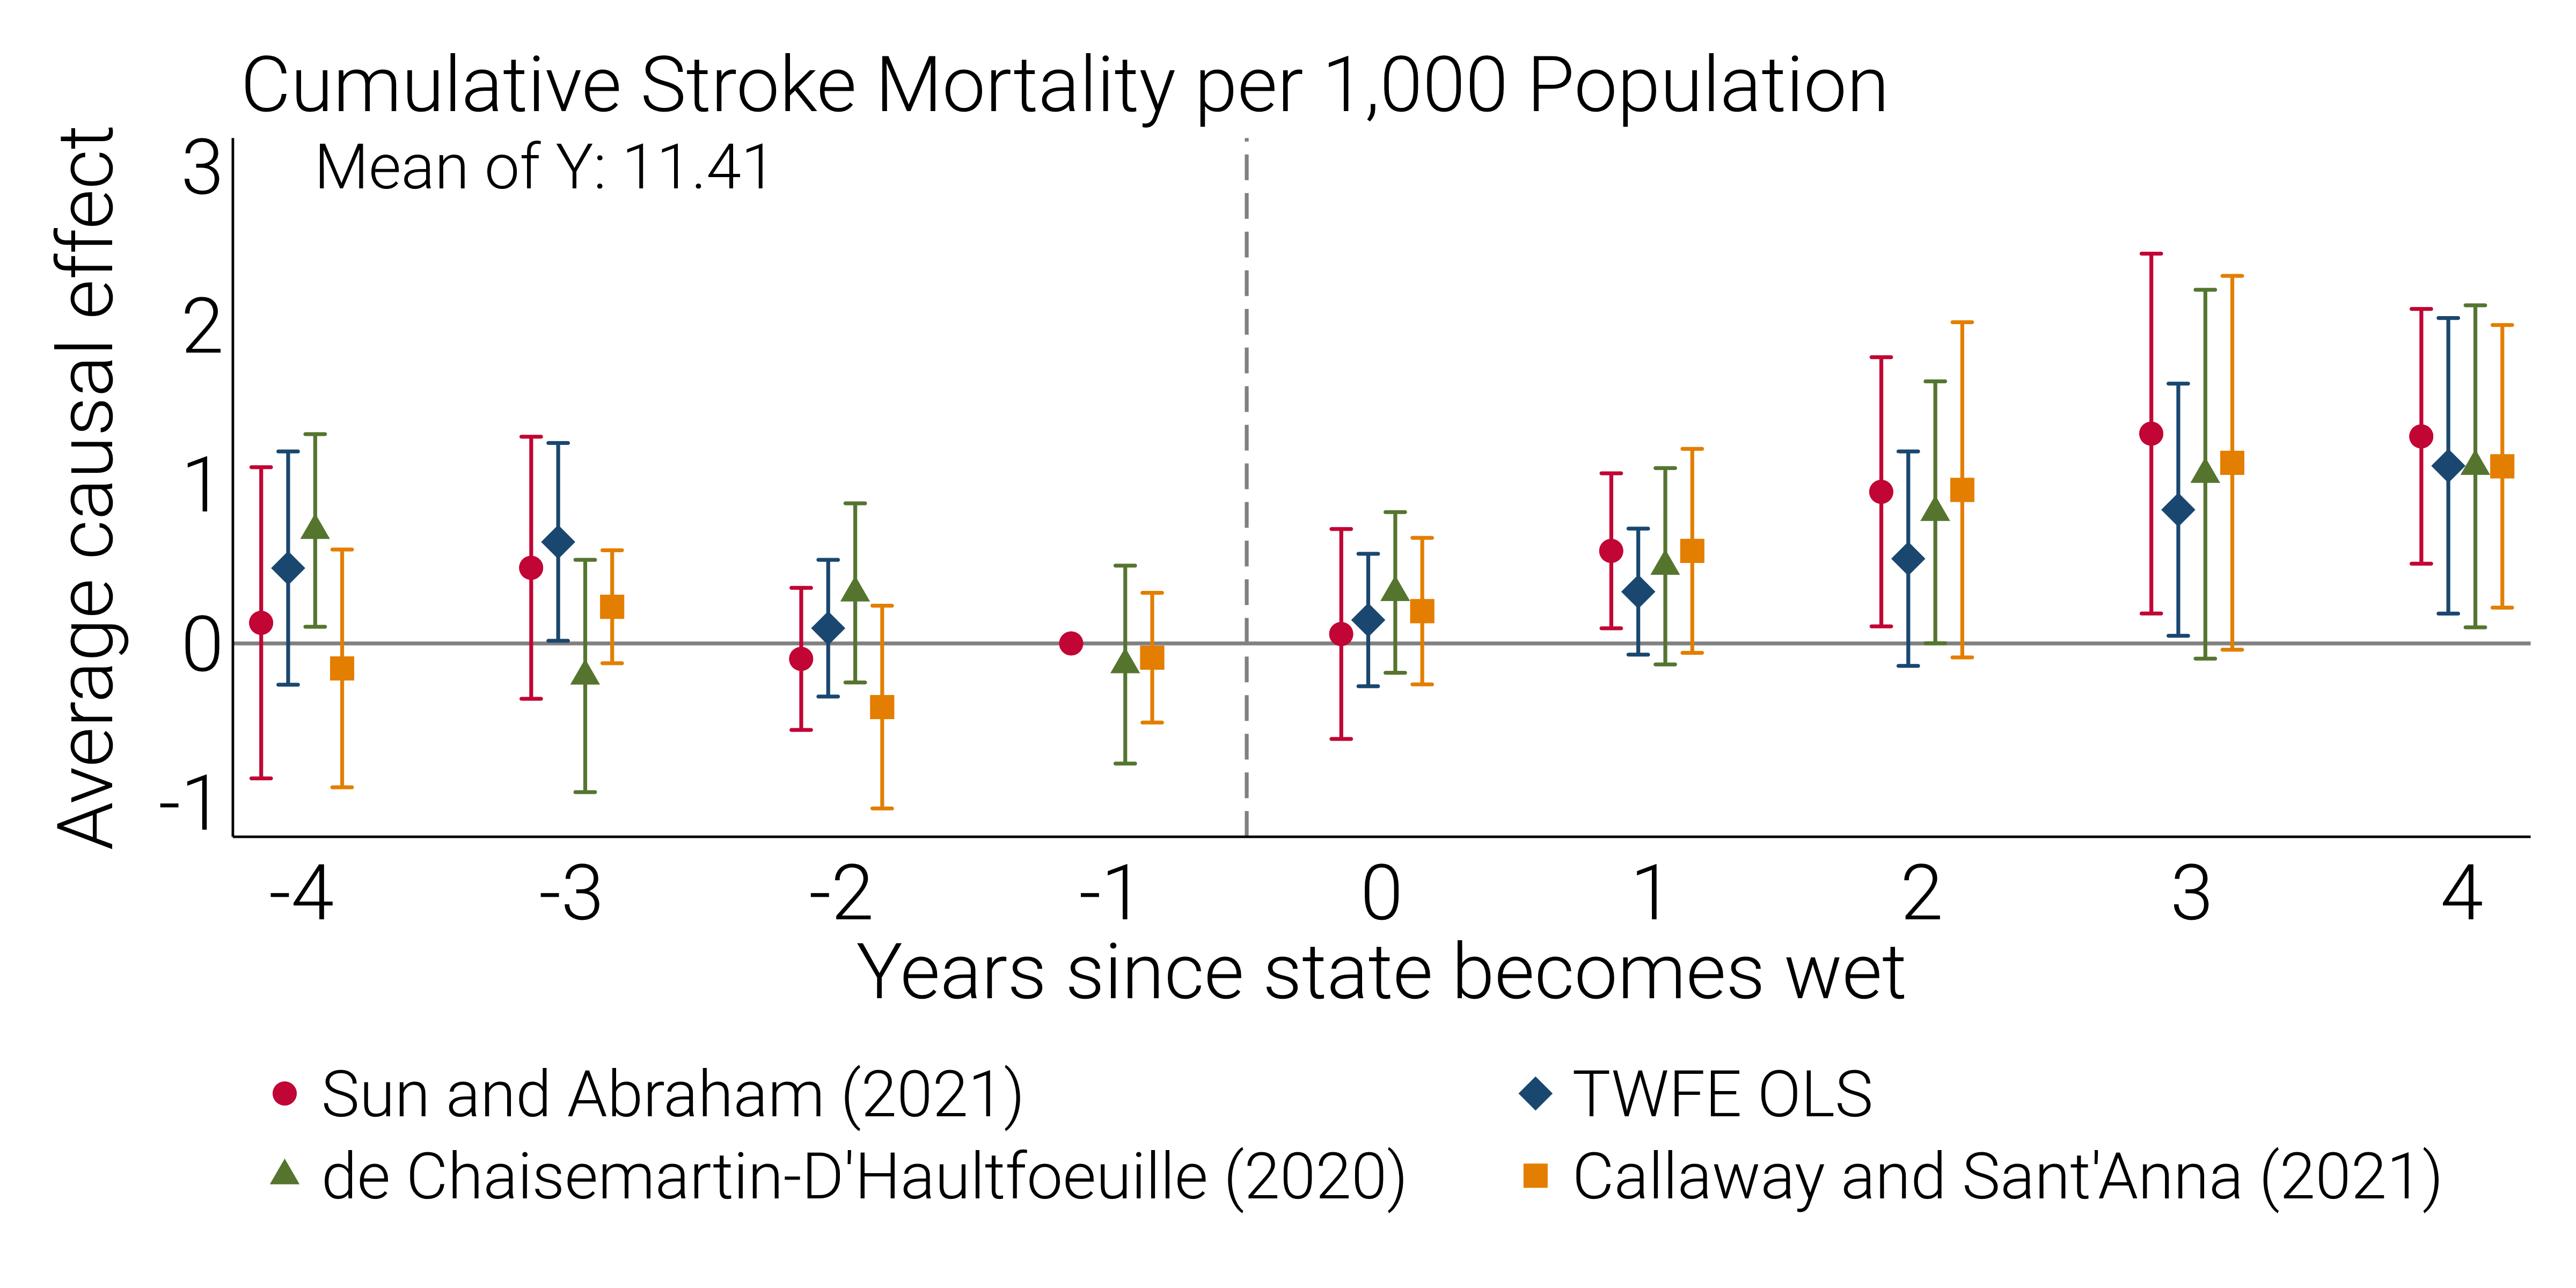
\includegraphics[width=1.0\linewidth]{../analysis/output/appendix/figure_d1c_es_cumulative_stroke.png}
    \end{subfigure}    
    \begin{subfigure}{0.47\linewidth}
        \centering 
        \caption[Cancer]{Cancer}        
        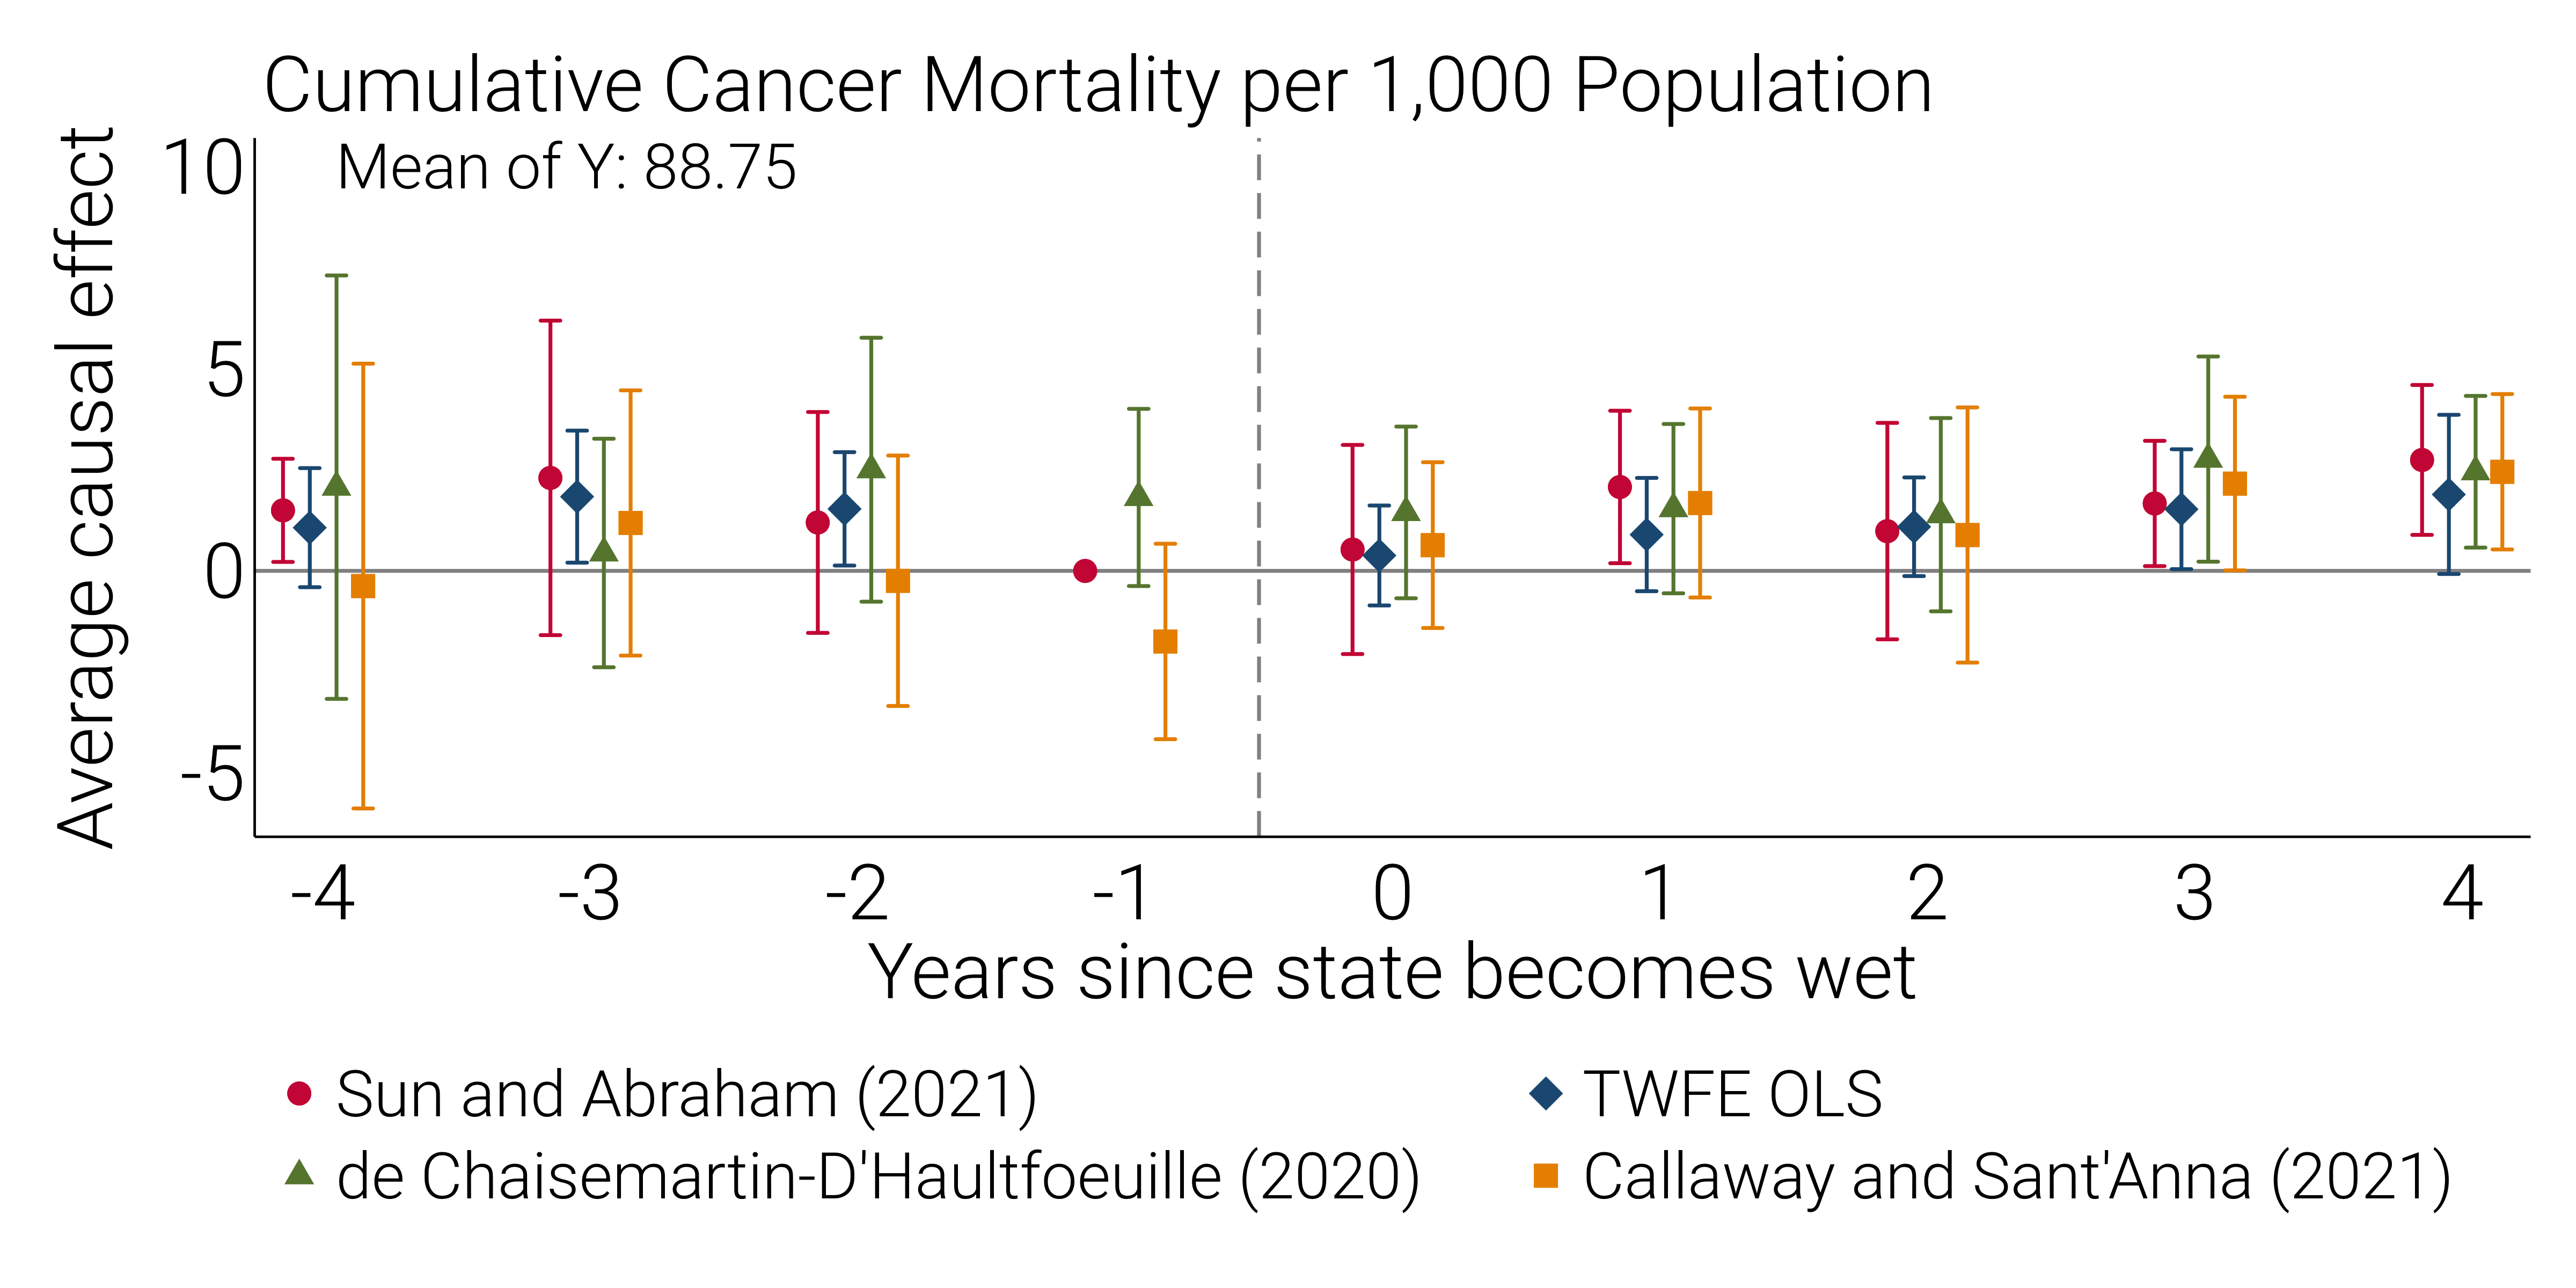
\includegraphics[width=1.0\linewidth]{../analysis/output/appendix/figure_d1d_es_cumulative_cancer.png}
    \end{subfigure}
    \Fnote{
        Each panel displays event studies with cumulative all-cause mortality (panel A) or cumulative cause-specific mortality between 1990 and 2004 per 1,000 population in 1990 as the dependent variable (heart disease in panel B, stroke in panel C, and cancer in panel D). 
        The unit of observation is a state of birth by year of birth cohort. 
        The sample includes the 1930 to 1941 birth cohorts. 
        The ``Mean of Y'' is the sample mean of the dependent variable for pre-treatment (1930-1933) birth cohorts in not-yet-treated states. 
        Each panel shows estimates based on \citeApp{sun_estimating_2021} and TWFE OLS as before as well as \citeApp{callaway_difference--differences_2021} and \citeApp{de_chaisemartin_two-way_2020}. 
        The coefficients for event-time periods $l = -8$ to $l = -5$ and $l = 5$ to $l = 7$ are omitted for clarity. 
        All specifications include the year of birth and state of birth fixed effects. 
        Observations are weighted by the surviving cohort size in 1990 for each state of birth by year of birth cohort. 
        Standard errors are clustered at the state of birth level.
    }
    \label{fig:event-study-cause-of-death-cumulative}
\end{figure}
\end{landscape}
\restoregeometry

% Table D1. Robustness of DiD to cumulative mortality
\begin{table}[!ht]\centering
  \begin{adjustbox}{width=1.0\textwidth}
  \centering
    \begin{threeparttable}
     \caption{Aggregate Event Study Estimates using Cumulative Mortality}
     \estauto{../analysis/output/appendix/table_d1_cumulative.tex}{4}{S[table-format=2.3,table-column-width=20mm, table-alignment = center]}
      \label{tab:did-cumulative-mortality}
      \Fignote{
            The unit of observation is a state of birth by year of birth cohort. 
            The sample includes the 1930 to 1941 birth cohorts. 
            The ``Mean of Y'' is the sample mean of the dependent variable for pre-treatment (1930-1933) birth cohorts in not-yet-treated states. 
            The dependent variable is cumulative all-cause deaths per 1,000 population (Column 1) or the number of cause-specific deaths from heart disease (Column 2), stroke (Column 3), or cancer (Column 4) between 1990 and 2004 per 1,000 population in 1990. 
            Each coefficient is the average of the \citeApp{sun_estimating_2021} event study coefficients from $l = 0$ to $l = 4$ and represents the average change in the later-life all-cause mortality rate attributable to in utero exposure to the first five years of federal prohibition’s repeal. 
            In all columns, observations are treated (i.e., the indicator for wet status equals one) if at least some alcohol sales were allowed anywhere within the state of birth in the year of birth. 
            In all specifications, mortality rates are a function of state of birth by death year and year of birth by death year fixed effects and control for the log of per capita New Deal spending and the log of per capita real disposable personal income at the state level. 
            Observations are weighted by the surviving cohort size in 1990 for each state of birth by year of birth cohort. 
            All standard errors are clustered at the state of birth level. 
            Standard errors are in parentheses; t-statistics reported below standard errors in brackets.
        }
    \end{threeparttable}
   \end{adjustbox}
\end{table}



%----------------------------------------------------%
%       Appendix E: Heterogeneity
%----------------------------------------------------%

\FloatBarrier
%\newpage 

\newgeometry{top = 0.5in, bottom = 0.5in, right = 0.5in, left = 0.5in, footskip = 0.0in}
\begin{landscape}

\section[Heterogeneity by Sex and Race]{Heterogeneity by Sex and Race\label{sec:app-het}}
\setcounter{table}{0}\renewcommand{\thetable}{\ref{sec:app-het}\arabic{table}}
\setcounter{figure}{0}\renewcommand{\thefigure}{\ref{sec:app-het}\arabic{figure}}

% Figure E1 - Event studies for Heterogeneity by Sex and Race
\begin{figure}[!ht]
    \caption[Event studies for Heterogeneity by Sex and Race]{Event studies for Heterogeneity by Sex and Race}
    \centering
    \begin{subfigure}{0.49\linewidth}
        \centering 
        \caption[Women]{Women}        
        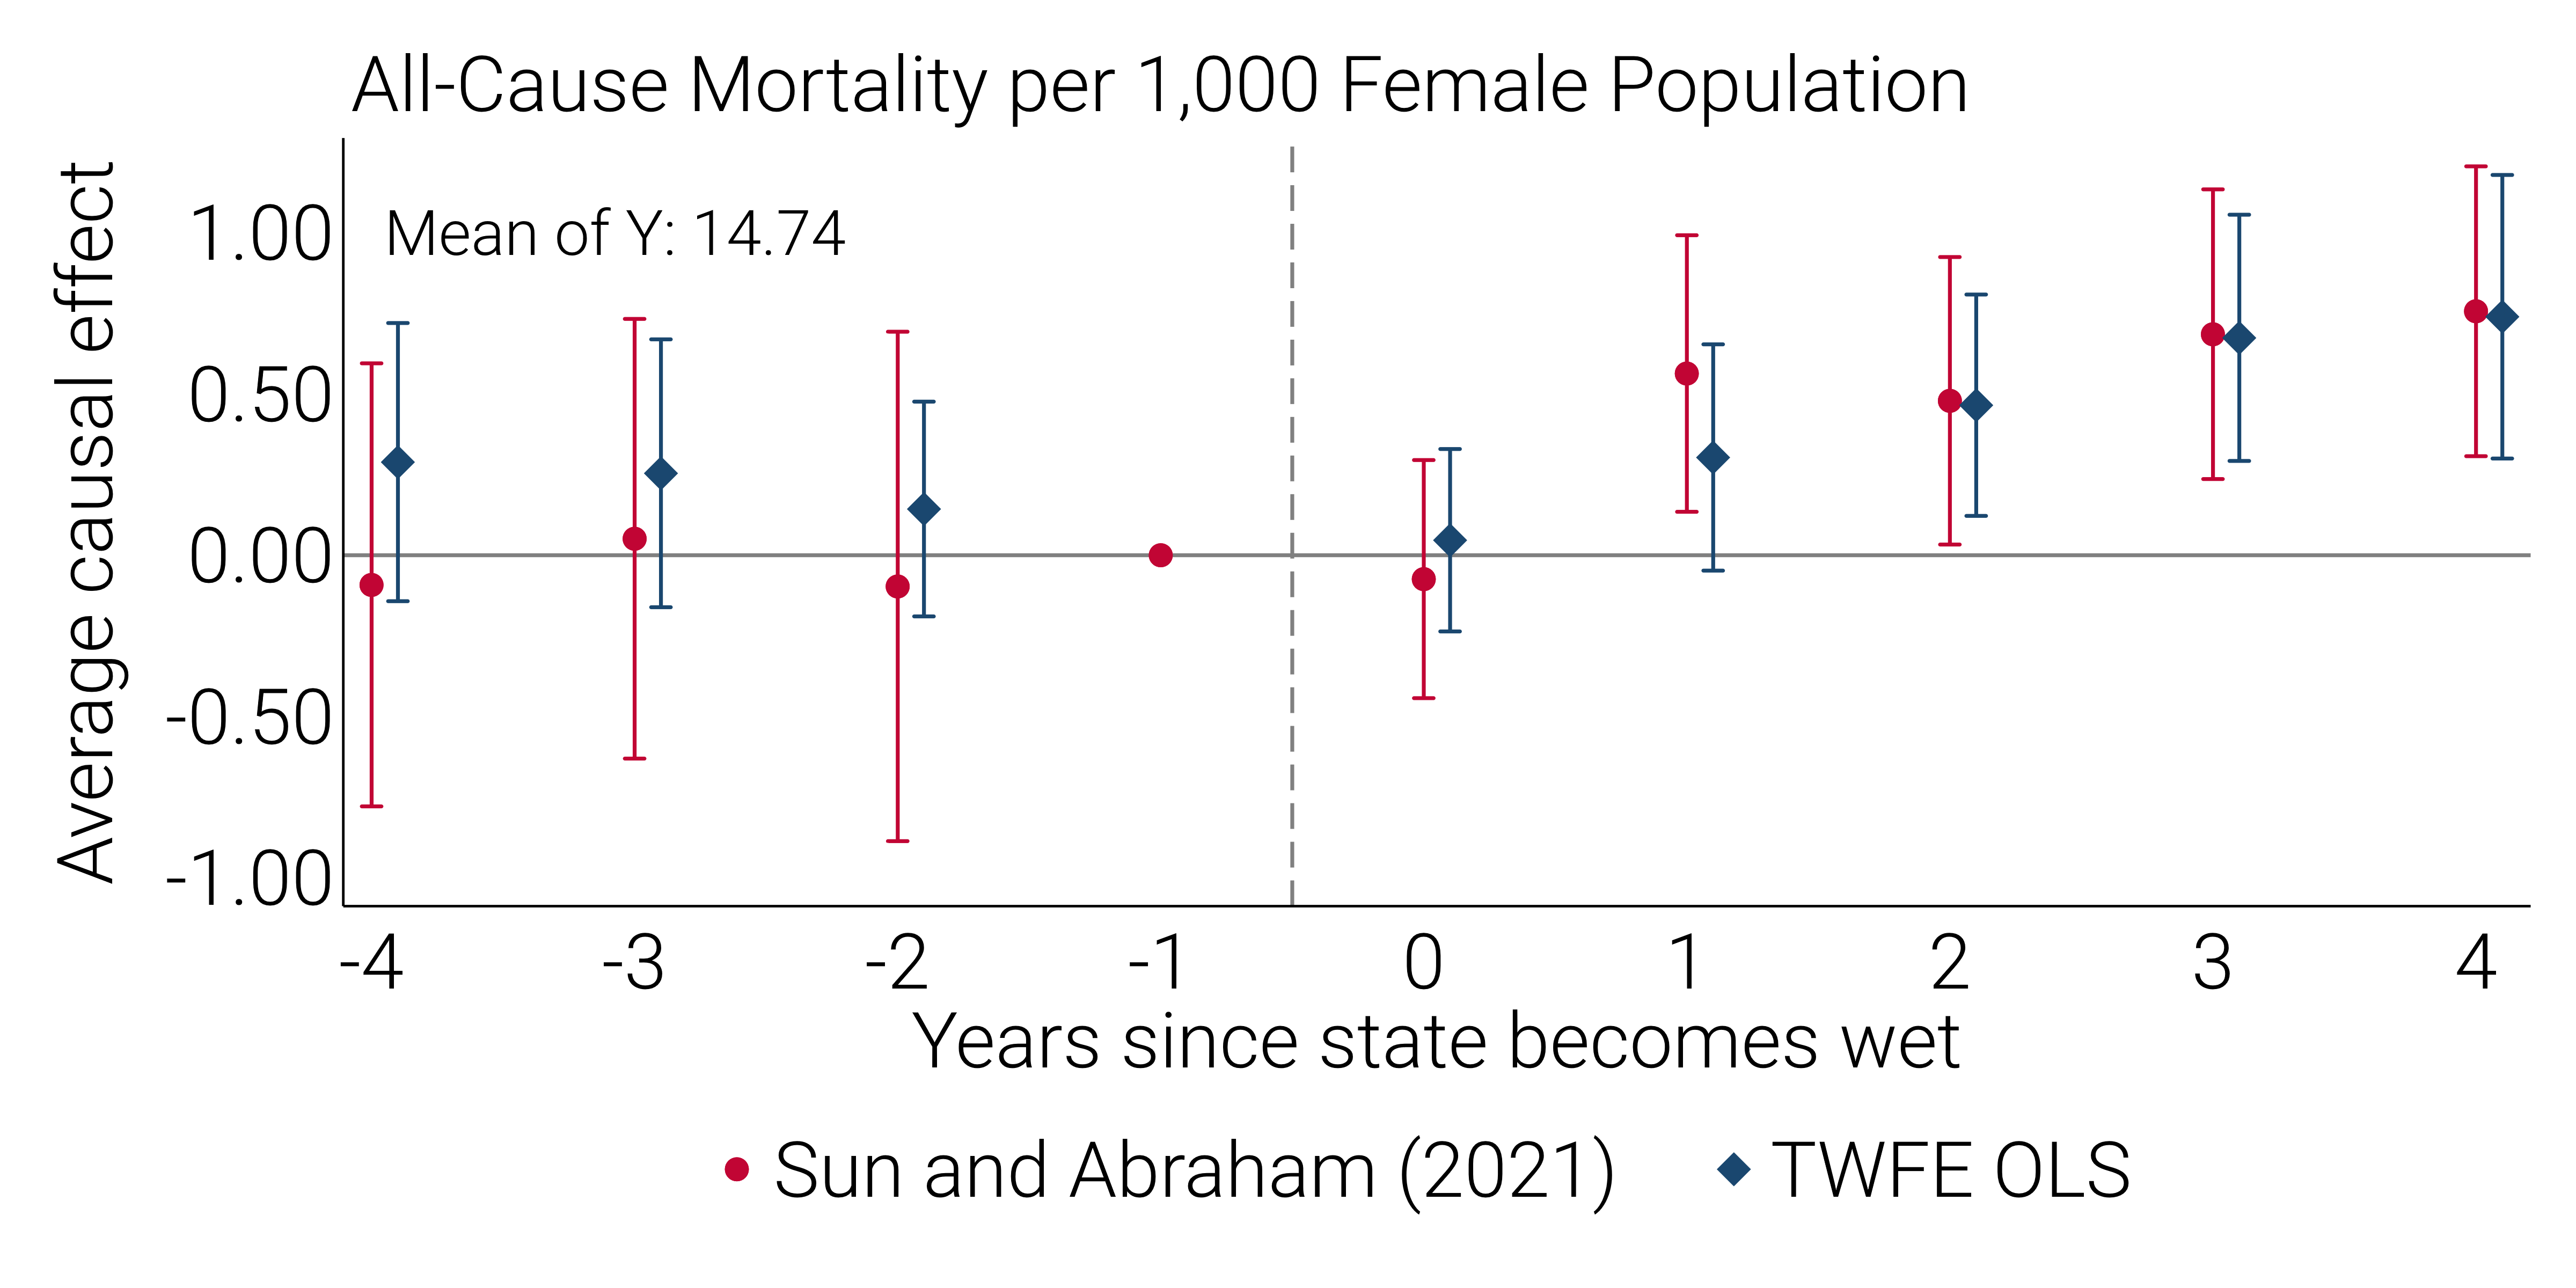
\includegraphics[width=1.0\linewidth]{../analysis/output/appendix/figure_e1a_event_study_women_only.png}
    \end{subfigure}
    \begin{subfigure}{0.49\linewidth}
        \centering 
        \caption[Men]{Men}        
        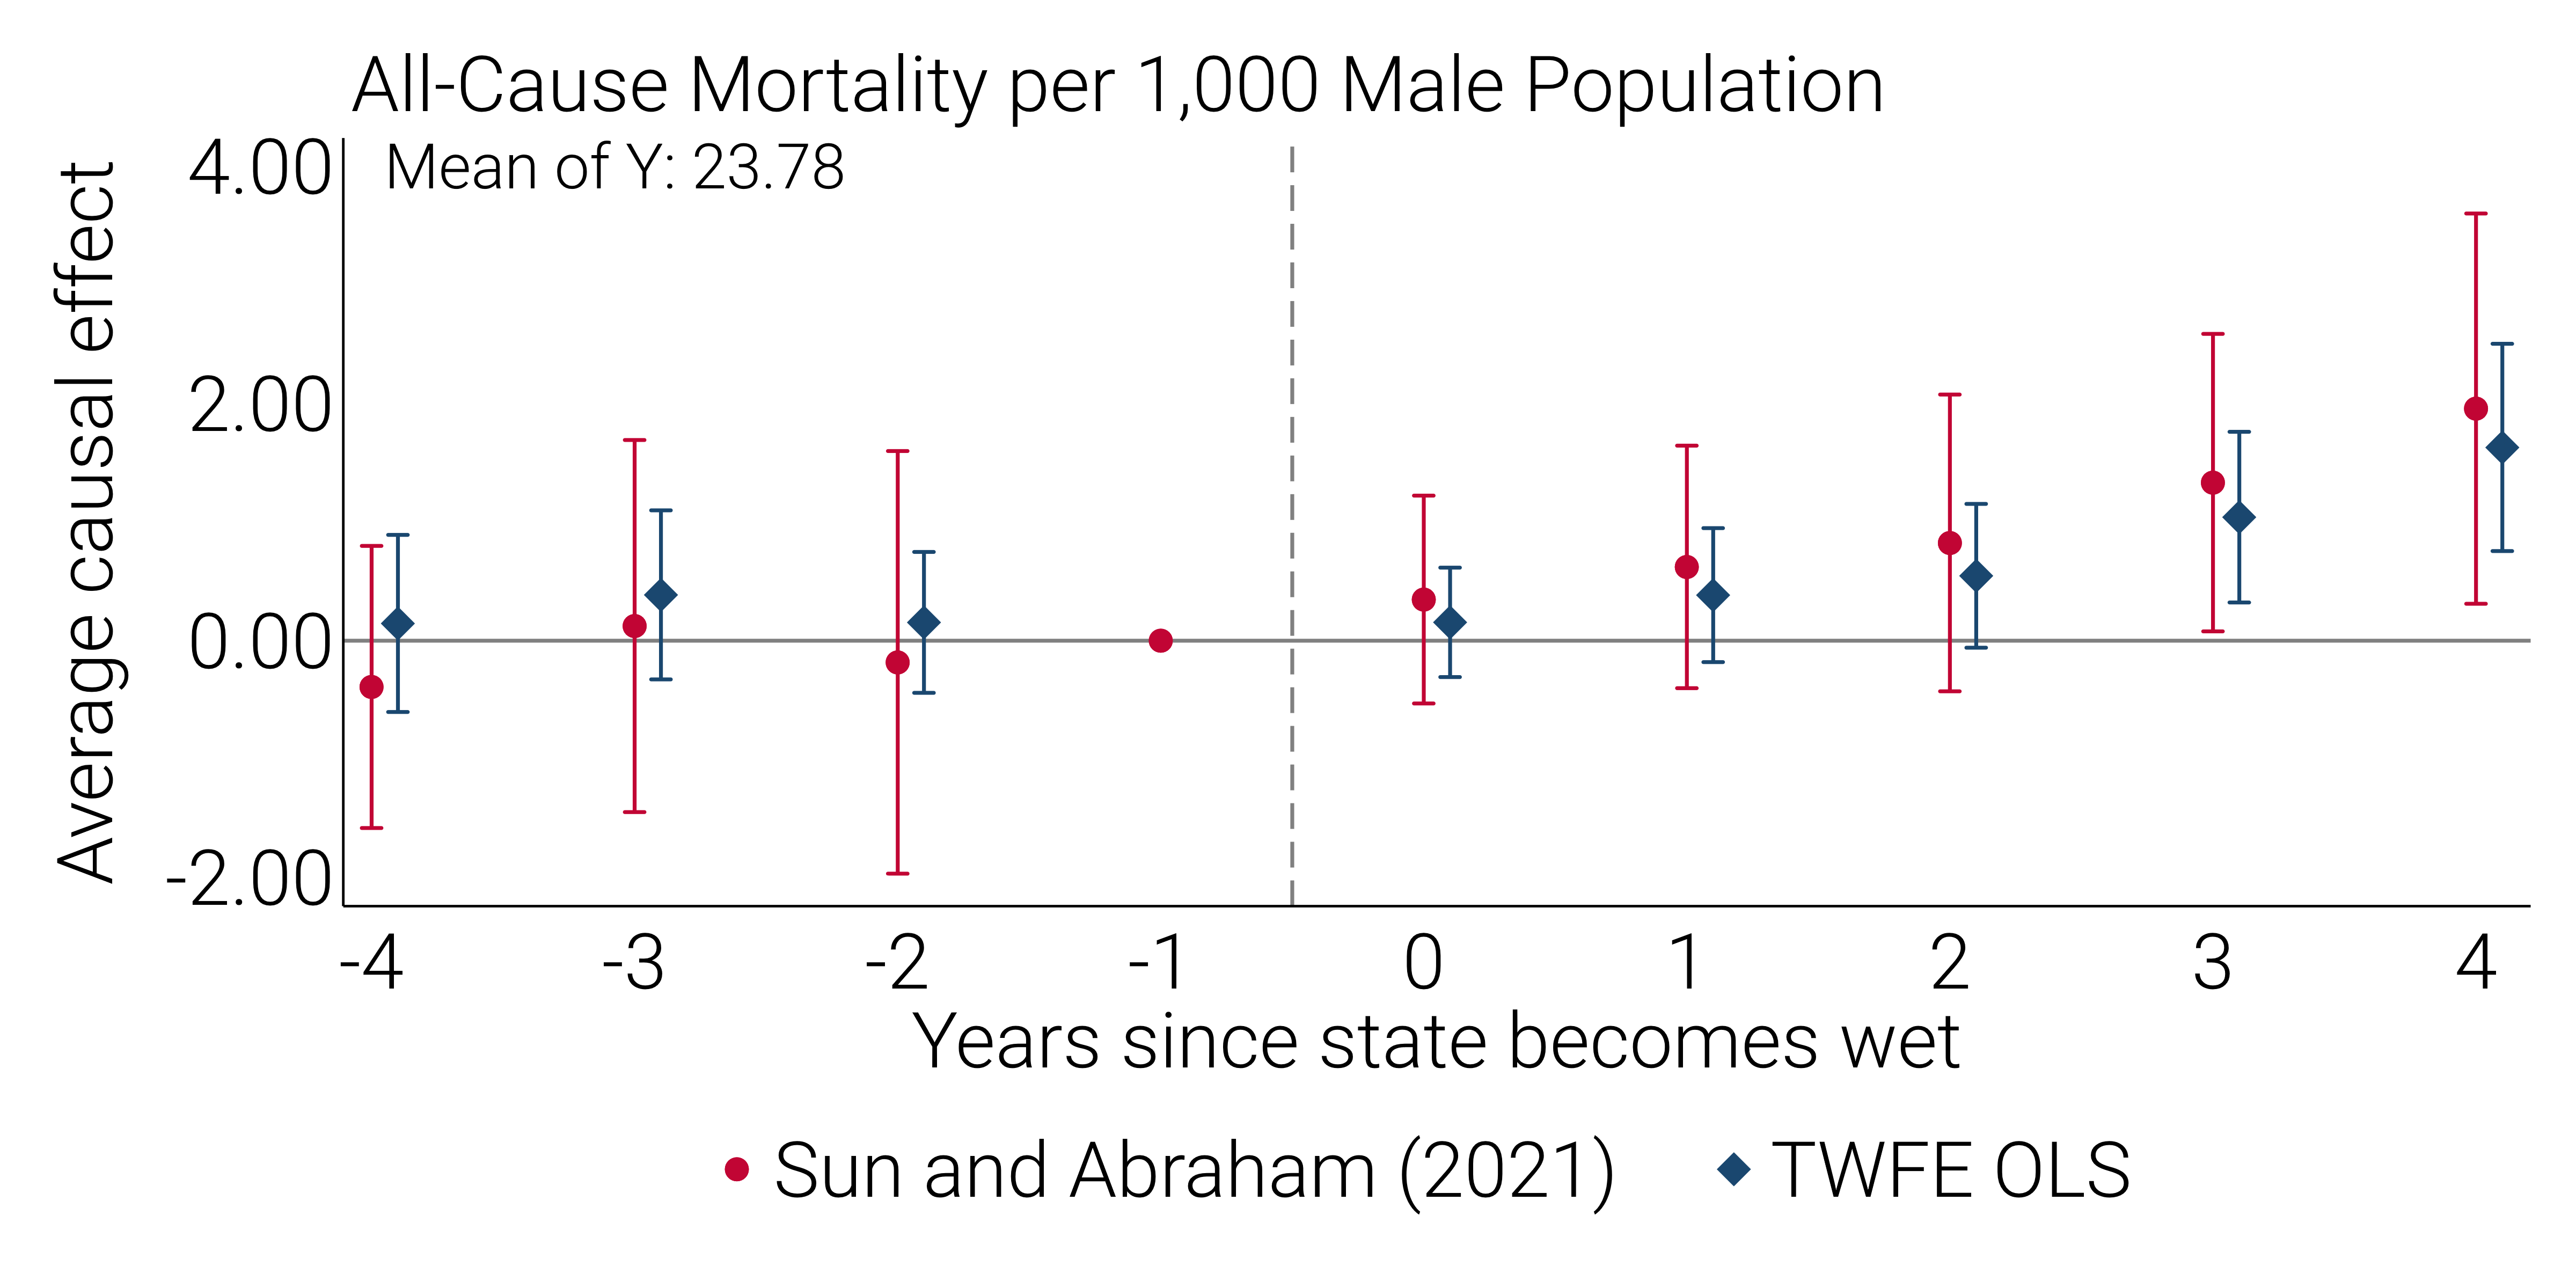
\includegraphics[width=1.0\linewidth]{../analysis/output/appendix/figure_e1b_event_study_men_only.png}
    \end{subfigure}
    \begin{subfigure}{0.49\linewidth}
        \centering 
        \caption[Non-White]{Non-White}        
        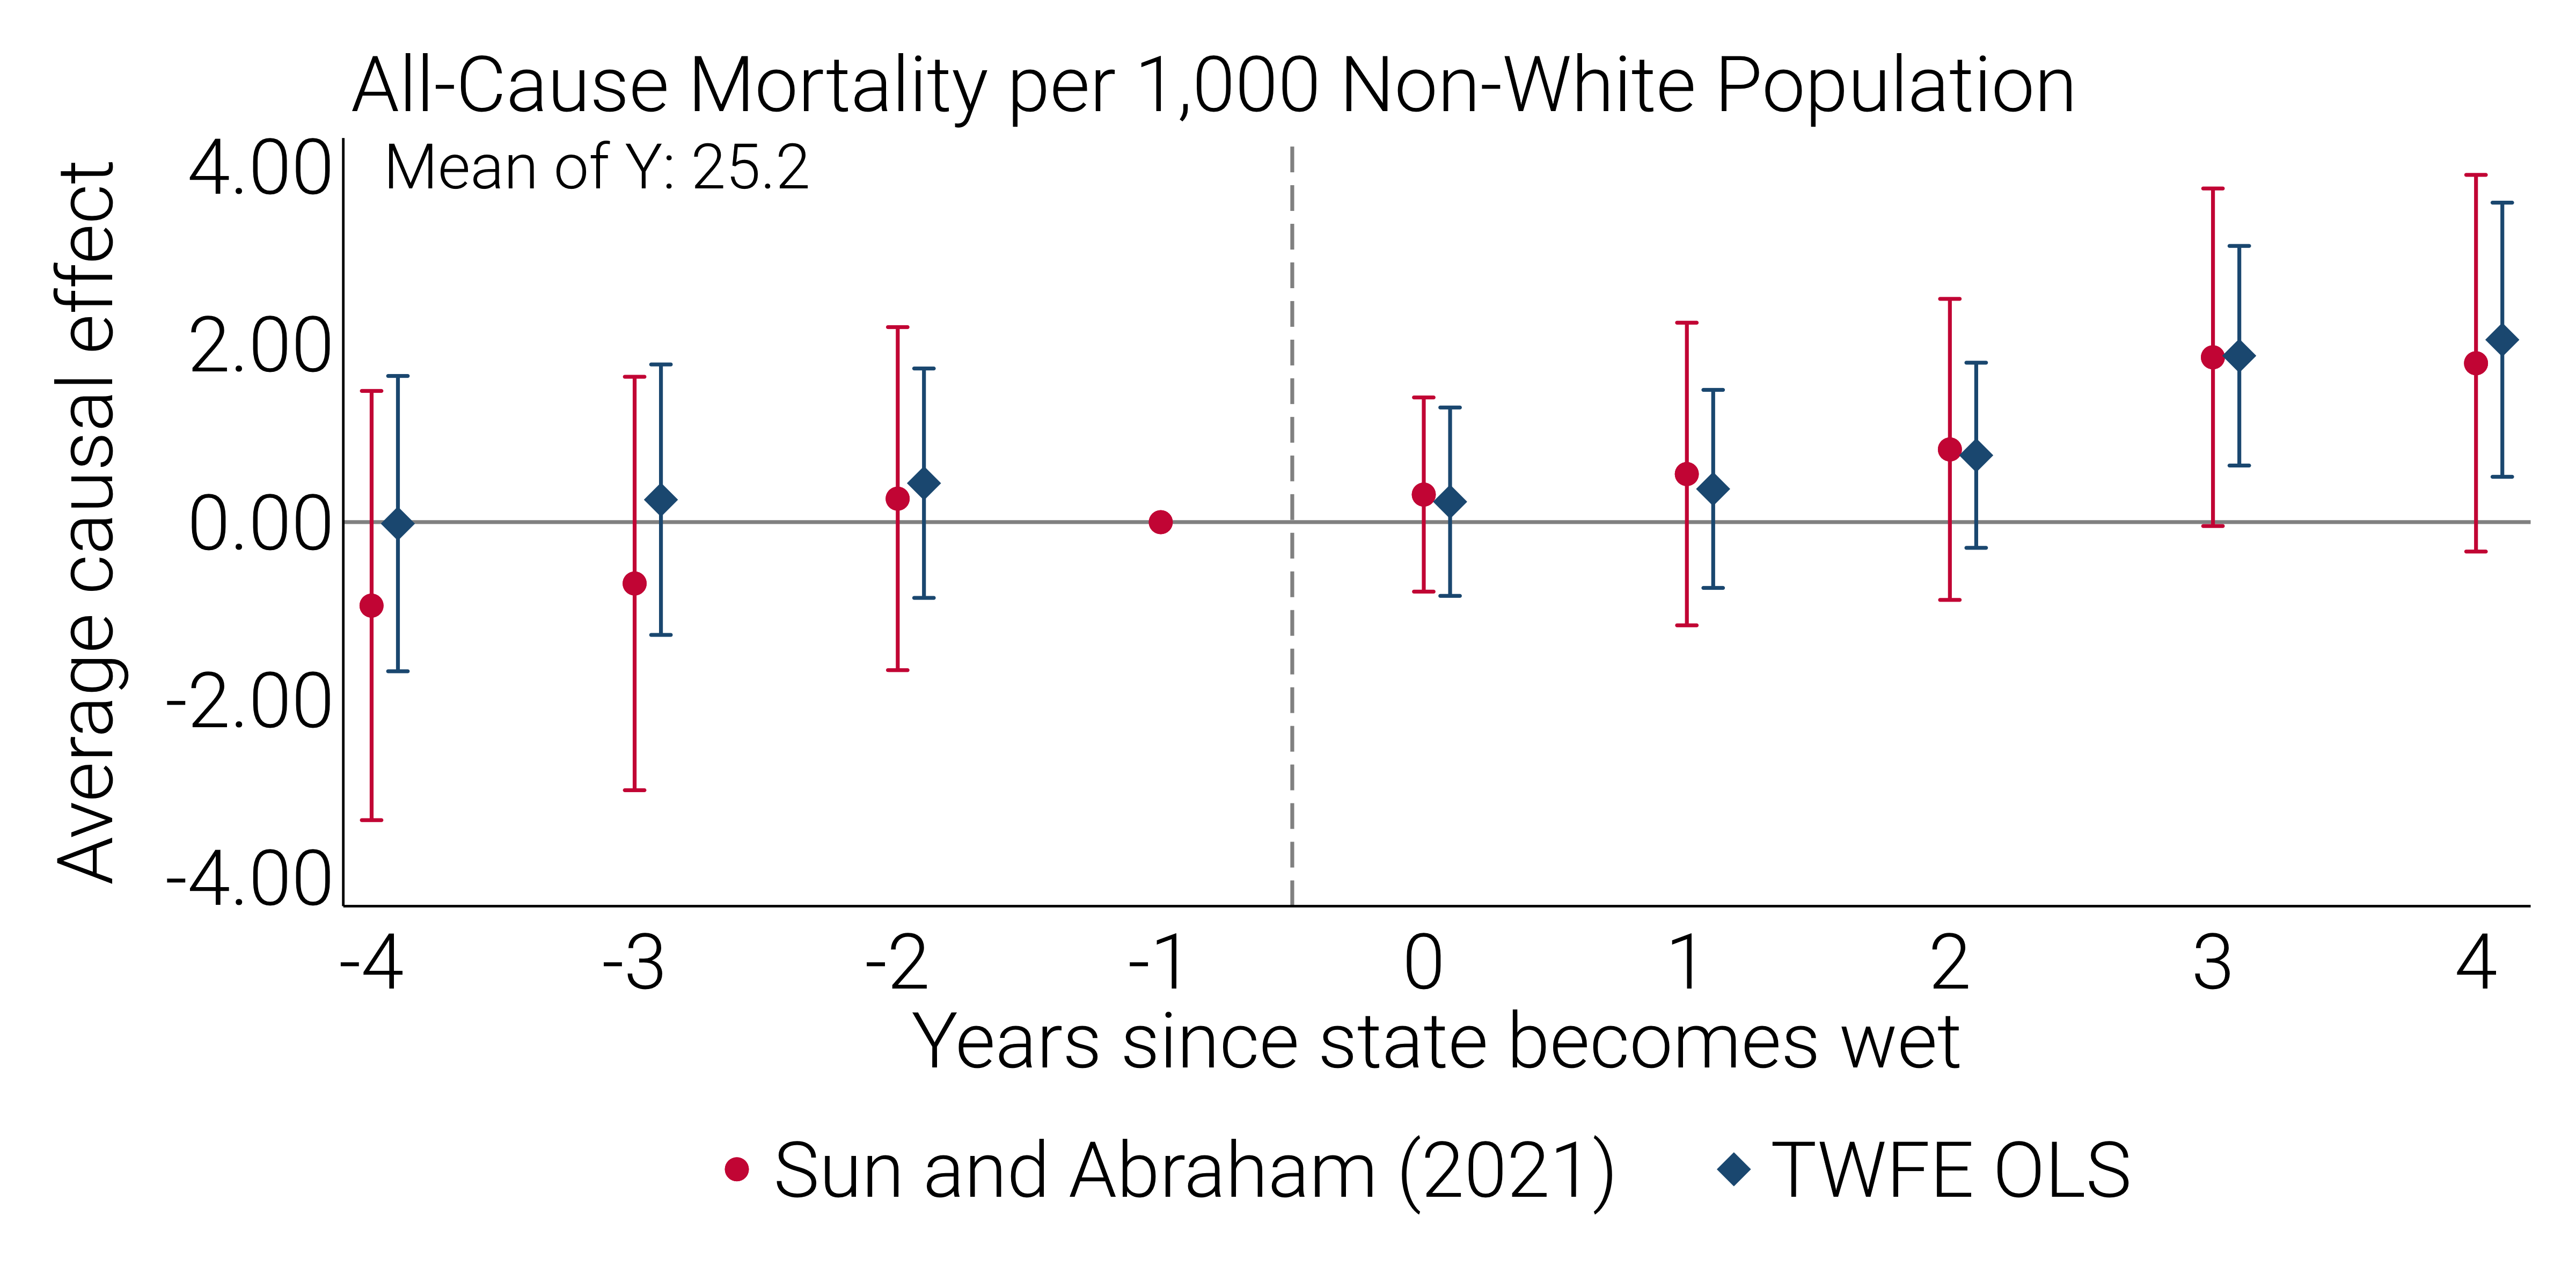
\includegraphics[width=1.0\linewidth]{../analysis/output/appendix/figure_e1c_event_study_non_white_only.png}
    \end{subfigure}
    \begin{subfigure}{0.49\linewidth}
        \centering 
        \caption[White]{White}        
        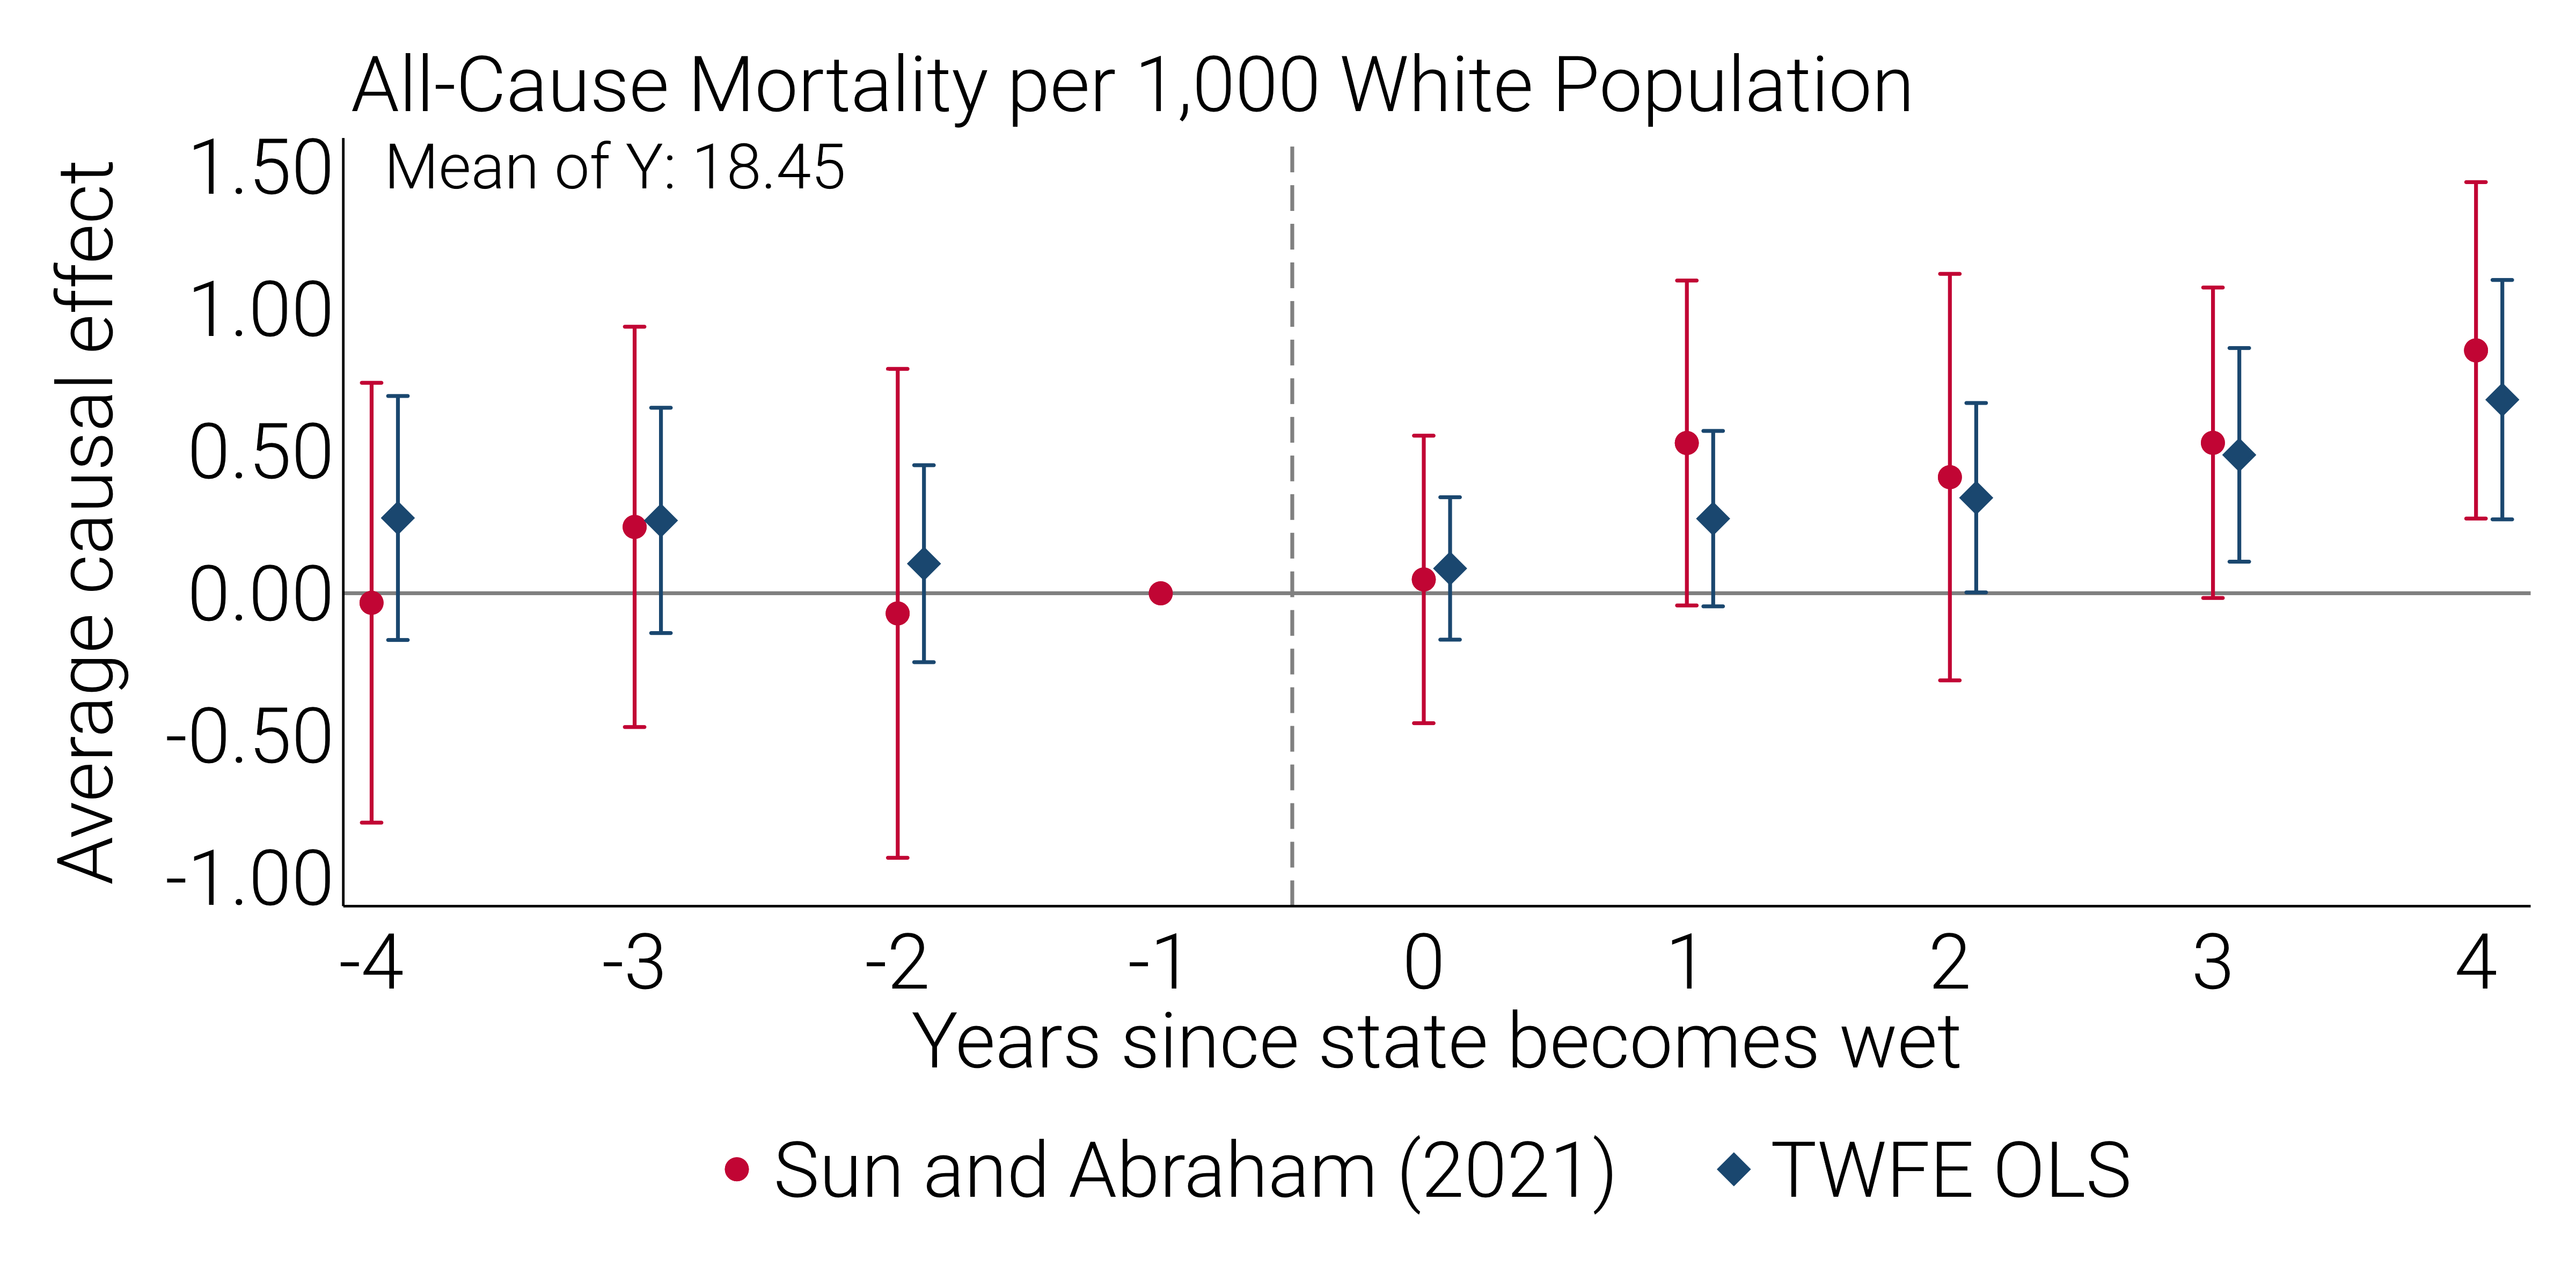
\includegraphics[width=1.0\linewidth]{../analysis/output/appendix/figure_e1d_event_study_white_only.png}
    \end{subfigure}
    \Fnote{
        Each panel displays event studies with all-cause mortality per 1,000 population as the dependent variable. 
        Panels A, B, C, and D do so for females, males, non-white people, and white people, respectively. 
        They all use the same clustering, estimation techniques, observation weighting, sample, and specification as those in Figure~\ref{fig:event-study-cause-of-death}.  
        See the note to Appendix Figure~\ref{fig:event-study-cause-of-death-robust-control} for more details.
    }
    \label{fig:event-study-heterogeneity}
\end{figure}
\end{landscape}
\restoregeometry

%------------------------------------------%
%               Appendix References
%------------------------------------------%
\newpage
\FloatBarrier
\setlength{\bibsep}{3pt}

\begin{spacing}{0}
\bibliographystyleApp{references/econ}
{\small\bibliographyApp{references/prohibition}{}}
\end{spacing}

\end{document}
